\documentclass[useAMS,usenatbib,usegraphicx]{mnras}
\usepackage{amsmath}
\usepackage{morefloats}
\usepackage{graphicx}

%%%%%%%%%%%%%%%%%%%%%%%%%%%%%%%%%%%%%%%%%%%%%%%%

\title[The first ten years of dust evolution in SN~1987A from 
optical line profile asymmetries]{Modelling supernova line profile asymmetries to determine ejecta dust masses:  SN~1987A from days 524 to 3640}
\author[Antonia Bevan and M. J. Barlow]{Antonia Bevan$^{1}$ and M. J. 
Barlow$^{1}$\\
$^{1}$Department of Physics and Astronomy, University College London, 
Gower Street, London WC1E 6BT, UK}

\begin{document}

\date{Accepted}

\pagerange{\pageref{firstpage}--\pageref{lastpage}} \pubyear{2015}

\maketitle

\label{firstpage}

%\begin{abstract}
%
%Unexpectedly large masses of dust up to $0.7M_{\odot}$ have been 
%discovered in the ejecta of SN 1987A.  These dust masses are based on 
%fitting the observed mid-IR and far-IR continuum.  In many 
%supernovae, line profiles in the optical and near-IR exhibit a red-blue 
%asymmetry as a result of greater extinction to radiation emitted from the 
%receding part of the supernova.  We  present here a new code, DAMOCLES, 
%that models the effects of dust on the line profiles of core-collapse 
%supernovae in order to determine the masses of newly formed dust.  We have 
%tested the code against previously published models and against analytical 
%results.  We find that the presence of a shoulder near the peak or an 
%extended red scattering wing in a line profile may also be suggestive of dust 
%formation.  We also note that dust-affected line profiles need not 
%necessarily be flux-biased towards to the blue. We have collated optical spectra of SN~1987A from a variety 
%of archives and sources and have modelled the evolution of the H$\alpha$ line from day 714 
%to day 3604.  We also present models of the blue-shifted 
%[O~{\sc i}]~$\lambda$6300,6363~\AA\ doublet bewteen days 714 and 1478.  We 
%conclude that a significant dust mass ($\sim 0.1M_{\odot}$) had 
%formed by day 3604 and infer that the majority of the present dust mass must 
%have formed after this epoch.  For pure amorphous carbon models, large grain 
%sizes ($\geqslant 0.6\mu$m; capable of surviving the reverse shock) are 
%required to fit the data even at early epochs (day 714).  Our 
%findings are in strong agreement with recent dust mass estimates for SED fits and confirm 
%the suggestion that the majority of SN~1987A dust formed many years after the 
%initial explosion.
%
%\end{abstract}


\begin{abstract}

The late time optical and near-IR line profiles of many core-collapse supernovae exhibit 
a red-blue asymmetry as a result of greater extinction by internal dust of 
radiation emitted from the receding parts of the supernova ejecta.  We 
present here a new code, DAMOCLES, that models the effects of dust on the 
line profiles of core-collapse supernovae in order to determine the masses 
of newly formed dust. We have tested the code against previously published 
models and against analytical results. We find that the presence of an 
extended red scattering wing in a line profile may also be indicative of 
dust formation and also that dust-affected line profiles need not 
necessarily be flux-biased towards to the blue, although the profile peak 
will always be blue-shifted. We have collated optical spectra of SN~1987A 
from a variety of archival sources and have modelled the evolution of the 
H$\alpha$ line from days 714 to 3604, as well as that of the [O~{\sc 
i}]~6300,6363~\AA\ doublet between days 714 and 1478. A variety of 
evidence points to the presence of clumping and we find that our clumped 
dust models require significantly higher dust masses than smoothly 
distributed dust models. Large grain radii ($\geqslant 0.6\mu$m) are 
required to fit the line profiles even at the earlier epochs.  We conclude 
that a large dust mass ($\sim 0.1M_{\odot}$) had formed by day 3604 and 
infer that the majority of the present dust mass must have formed after 
this epoch. Our findings are in agreement with recent estimates from SED 
fits for the dust mass evolution of SN~1987A and confirm that the majority 
of SN~1987A's dust formed many years after the initial explosion.

\end{abstract}

\begin{keywords}
supernovae: general  -  supernovae: individual: SN 1987A  -  ISM: 
supernova remnants  - radiative transfer
\end{keywords}


%%%%%%%%%%%%%%%%%%    INTRODUCTION     %%%%%%%%%%%%%%%%%%%%%
\section{Introduction}

%Core-collapse supernovae have long been thought to be potential dust 
%factories.  Over the past decade, observations in the IR have suggested 
%that the quantities of dust produced are too low to account for the masses 
%measured in the early universe.  However, recent Herschel and Planck 
%far-IR and sub-mm observations of massive dust reservoirs (as high as 
%0.7$M_{\odot}$) have resulted in a reevaluation of the rate of dust 
%production in these objects \citep{Barlow2010, Matsuura2011, Gomez2012}.  These estimates are based on fitting the observed mid-IR 
%and far-IR continuum. Following the end of the Herschel mission in April 
%2013 there is now a long wait for comparable or better spaceborne thermal 
%IR facilities to become available, with the next major IR mission SPICA 
%%\citep{SPICA} not due to launch until 2022.  However, insight may still 
%be gained via other means.
%   
%The absorption and scattering of optical or near-IR radiation by 
%newly-formed dust within the ejecta of supernovae can result in an 
%asymmetry between the red and blue shifted components, with redwards 
%emission from the far side of the ejecta undergoing greater absorption.  
%\citet{Lucy1989} identified a line asymmetry in the [O~{\sc i}]~$\lambda$6300,6363~\AA\ doublet
%from SN~1987A between 5 August 1988 and 3 March 1989, where the later 
%spectrum was blue-shifted by $\sim 600 $~km~s$^{-1}$. Since then, such 
%red-blue asymmetries have been frequently observed in the late-time 
%($ > 400$ days) spectra of supernova ejecta and there is a large database of 
%these observations 
%available\citep{Lucy1989,Fabbri2011,Mauerhan2012,Milisavljevic2012}.

%%%%%%%%%MIKE NEW STUFF EDIT BEGIN %%%%%%%%%%%%
Core-collapse supernovae (CCSNe) have long been thought to be potential 
dust factories \citep{Hoyle1970, Kozasa1991, Todini2001}. However 
over the past decade observations at mid-infrared (mid-IR) wavelengths of 
warm dust emission from CCSNe had suggested that the quantities of dust 
produced, typically $\leq$ 10$^{-3}$~M$_\odot$ during the first 1000 days 
\citep{Sugerman2006, Meikle2007, Kotak2009, Andrews2010, Fabbri2011} were 
much less than the 0.1-1.0~M$_\odot$ of dust per CCSN that had been 
estimated to be needed \citep{Morgan2003, Dwek2007} in order to account 
for the very large dust masses measured in some high redshift galaxies 
\citep{Omont2001, Bertoldi2003, Watson2015}. However, recent {\em 
Herschel} far-IR and sub-mm observations of cold dust masses as high as 
0.2-0.8$M_{\odot}$ in several young supernova remnants have resulted in a 
re-evaluation of the rate of dust production by CCSNe \citep{Barlow2010, 
Matsuura2011, Gomez2012}. The {\em Hershel} dust mass estimates were based 
on fitting dust spectral energy distributions (SEDs) that peaked at far-IR 
wavelengths. Following the end of the {\em Herschel} mission in 
2013 there is likely to be a long wait for far-IR facilities with 
comparable or better sensitivities than {\em Herschel} to become 
available, providing an incentive to make use of alternative methods to 
estimate the dust masses that form in supernova ejecta.


The absorption and scattering of optical or near-IR radiation by 
newly-formed dust within the ejecta of supernovae can result in an 
asymmetry between the red and blue shifted components, with redwards 
emission from the far side of the ejecta undergoing greater absorption. 
\citet{Lucy1989} identified a progressive blue-shifting of the [O~{\sc 
i}]~$\lambda$6300,6363~\AA\ doublet from SN~1987A between days 529 and 739 
after outburst, with the doublet in the later spectrum being blue-shifted 
by $\sim 600 $~km~s$^{-1}$. Since then, such red-blue asymmetries have 
been frequently observed in the late-time ($ > 400$ days) spectra of 
supernova ejecta and there is now a growing database of such observations 
\citep{Lucy1989,Fabbri2011,Mauerhan2012,Milisavljevic2012}.

SN~1987A as an archetypal object is critical to our growing understanding 
of the formation and evolution of dust in CCSNe.  Since its outburst there 
have been numerous observations at many wavelengths and many epochs. 
Mid-infrared emission from warm dust (T$\sim$400~K) was observed by day 
$\sim$450 \citep{Roche1989, Bouchet1991, Wooden1993} and by day 775 the 
emitting dust mass was estimated to have been 
$\sim5-20\times10^{-4}$~M$_\odot$ \citep{Wooden1993, Ercolano2007, 
Wesson2015}. Beginning from 23 years after outburst, the {\em Herschel 
Space Observatory} detected much larger quantities 
(0.4-0.8~M$_\odot$M$_\odot$ of T$\sim$20~K cold dust emitting at far-IR 
and submillimetre wavelengths \citep{Matsuura2011, Matsuura2015}. This 
emission has been confirmed by ALMA observations to originate from the 
ejecta of SN~1987A \citep{Indebetouw2014}.
%%%%% MIKE NEW STUFF END%%%%%%

%SN 1987A is an archetypal object that is not only fascinating but critical to our 
%growing understanding of the formation and evolution of dust in core 
%collapse supernovae.  There have been numerous observations at all 
%wavelength ranges and at all epochs. Blue-shifted lines are frequently 
%observed in the spectrum.  It has been deduced that very large masses of 
%dust have formed within the ejecta of SN 1987A 
%but until recently the rate of dust formation in this object had been 
%unclear \citep{Matsuura2011}.  Recent modelling by \citet{Wesson2015} (hereafter W15) has 
%provided some of the first clear insights into the rate of dust formation 
%in the ejecta of SN 1987A.

We here seek to model  the effects of dust on line profiles with a 
view to providing both an alternative way of determining dust 
masses formed in the ejecta of core-collapse supernovae and in order to investigate 
the  effects of dust on the shapes of line profiles emitted from 
these objects.  We present a new code, DAMOCLES (Dust Affected Models Of 
Characteristic Line Emission in Supernovae), that utilises a Monte Carlo 
methodology in order to  model line profiles in expanding 
atmospheres.  The code can treat dust composed of multiple species 
and grain sizes with variable ejecta density and velocity distributions.  Both 
clumped and smooth geometries may be modelled.

%FIGURE
\begin{figure}
%\begin{center}
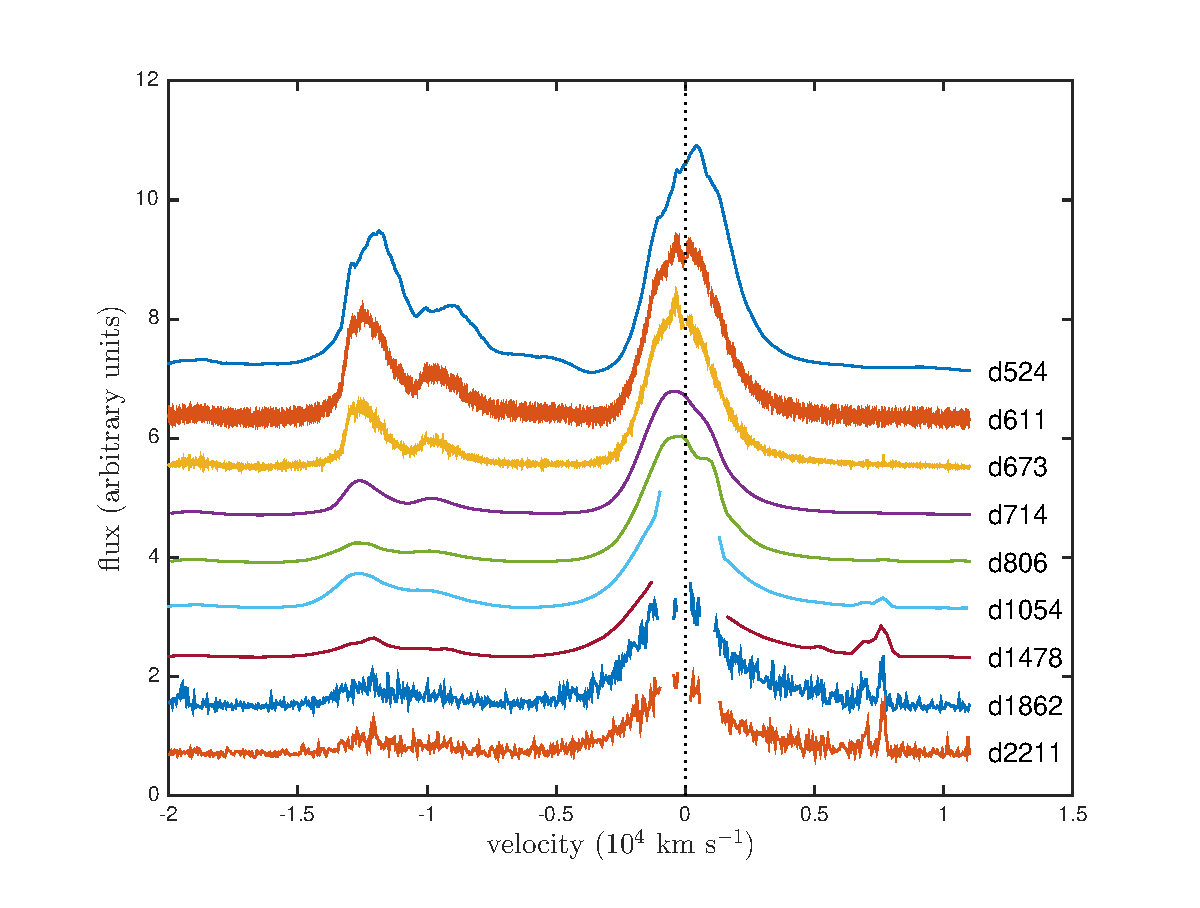
\includegraphics[trim =39 10 45 15,clip=true,scale=0.51]{Ha_evol_early_1col2}
\caption{Archival data showing the evolution of the H$\alpha$ and
[O~{\sc i}] line profiles from SN~1987A at the earlier of the epochs considered. The 
spectral gaps at the last two epochs correspond to where narrow line 
emission from the equatorial ring has been removed. The spectra have been
continuum-subtracted and offsets have ben applied for display purposes.}
\label{Ha_evol_early}
%\end{center}
\end{figure}
%FIGURE

In this paper we collate optical spectra from the archives of four 
different telescopes in order to study the effects of dust formation on 
the H$\alpha$ line and the [O~{\sc i}]~$\lambda$6300,6363~\AA\ doublet.  
We model epochs spanning a range of approximately 8 years 
from the first indications of blue-shifting in the H$\alpha$ line at 
$\sim$day 700, using both smooth and clumped geometries.  We compare our 
derived dust masses to those obtained by W15 and consider the implied dust
formation rate.  We present our testing of the new code against 
analytical cases and previously published optically thick models \citep{Lucy1989}. 
We also investigate 
the sensitivity of line profiles to each of the variables and 
 note the range of signatures that observed line profiles may exhibit 
in the presence of dust.

In Section \ref{spectra} we detail the observed spectra that we used for our 
modelling.  In Section \ref{code} we discuss the details of the DAMOCLES 
code and in Section \ref{params} we present our testing of the code and our parameter sensitivity 
analyses.  Our modelling of the H$\alpha$ and 
[O~{\sc i}]~$\lambda$6300,6363~\AA\ lines is presented in Section 
\ref{results} and  we discuss our findings in Section \ref{discuss}.


%%%%%%%%%%%%%%%%%%%%   INTRODUCTION   %%%%%%%%%%%%%%%%%%%%%%%%%%%

%FIGURE
\begin{figure}
%\begin{center}
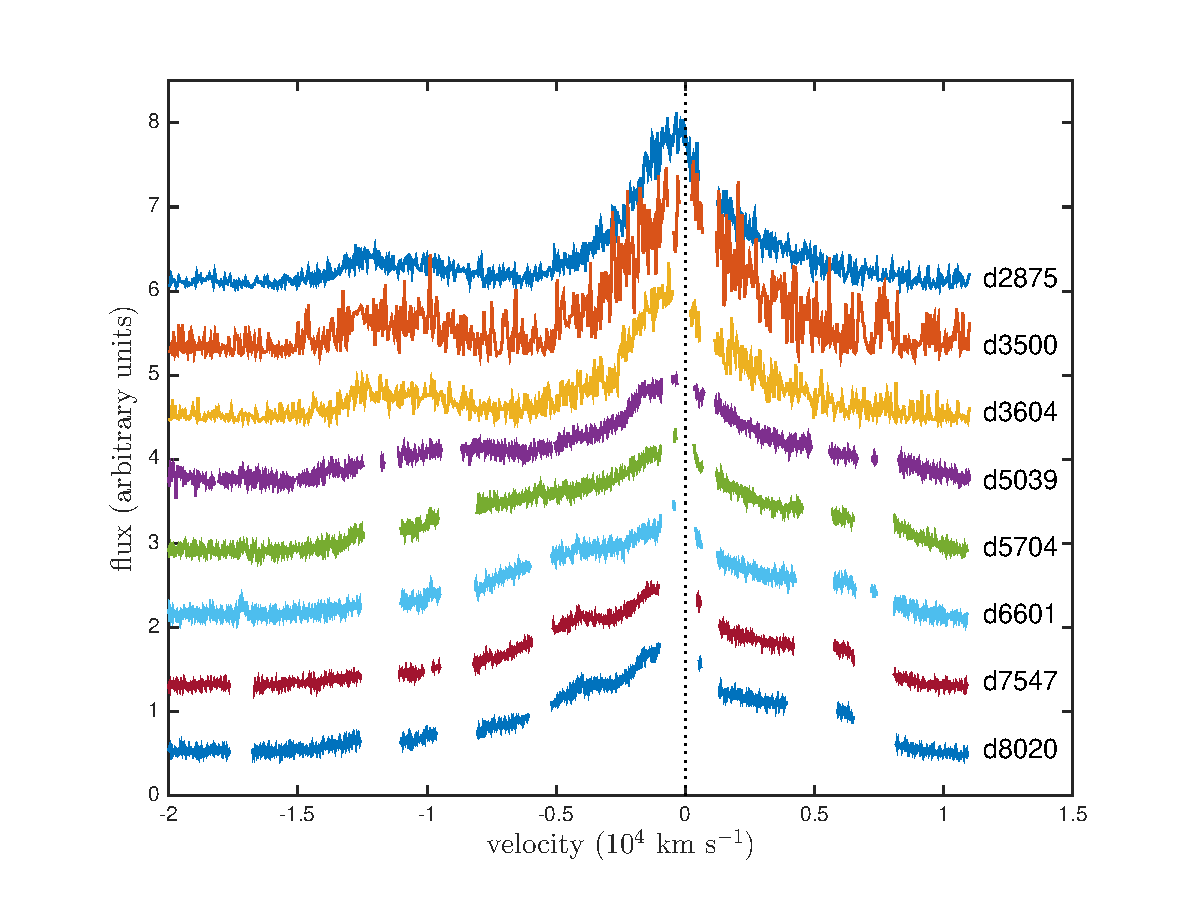
\includegraphics[trim =45 10 45 15,clip=true,scale=0.51]{Ha_evol_late_1col}
\caption{Archival data showing the evolution of the H$\alpha$
line profile from SN~1987A at the later epochs. The spectral gaps 
correspond to where narrow line emission from the equatorial ring has been 
removed. The spectra have been continuum-subtracted and offsets applied 
for display purposes.}
\label{Ha_evol_late}
%\end{center}
\end{figure}
%FIGURE

%%%%%%%%%%%%%%%%%%%%   SPECTRA   %%%%%%%%%%%%%%%%%%%%%%%%%%%

\section{Archival spectra of SN 1987A}
\label{spectra}

SN~1987A has been the most intensively observed supernova in history, with 
a wealth of both spectral and photometric data available to model.  From 
the archives of a number of different telescopes we have collated optical 
spectra acquired over a wide range of epochs.  At the earlier epochs we 
use spectra obtained by the Anglo-Australian Telescope (AAT) and the Cerro 
Tololo Inter-American Observatory (CTIO) and at later epochs we 
use spectra from the archives of the Hubble Space Telescope (HST) and the Very 
Large Telescope (VLT).  An explosion date of 23 February 1987 is adopted 
throughout and epochs are measured relative to this date.  Full details of 
all observations may be found in Table \ref{tb:data}. The spectral 
resolutions of the grating spectrograph observations are listed in 
column~7, while column~8 lists the spectral resolving powers of the 
echelle spectrograph observations.

Wavelength ranges encompassing the H$\alpha$ line and [O~{\sc i}]~$\lambda$6300,6363~\AA\ doublet were selected in order to trace their 
evolution from day 524, near the time of the first indications of dust 
formation \citep{Wooden1993}, to day 8020, near the current era. Optical 
spectroscopy obtained at the AAT using the Faint Object Red Spectrogaph 
(FORS) during the first two years after outburst was kindly supplied by Dr Raylee 
Stathakis \citep{Spyromilio1991, Spyromilio1993, Hanuschik1993} and optical spectra from the CTIO donated by Dr Mark Phillips \citep{Suntzeff1991}.

\begin{table*}
	\begin{minipage}{180mm}
	\caption{Details of the archival data for SN 1987A.}
	\label{tb:data}
  	\begin{tabular}{@{} ccccccccl @{}}
    	\hline
	Date & Age & Telescope  & Inst & $\lambda_{min}$ & $\lambda_{max}$ & Res. & Res. Power & Reference \\
	& (days) & & &(\AA) & (\AA)& (\AA)\\
	\hline
31 Jul 1988 & 524 & AAT & FORS & 5500 & 10190 & 20 & & \citet{Spyromilio1991} \\
26 Oct 1988 & 611 & AAT & UCLES & 6011 & 7336 &  & 30000 & \citet{Hanuschik1993, Spyromilio1993}\\
27 Dec 1988 & 673 & AAT & UCLES & 5702 & 10190 &  & 30000 & \citet{Hanuschik1993, Spyromilio1993}\\
06 Feb 1989 & 714 & CTIO-1.5m & Cass. & 6420 & 10380 & 16 & & \citet{Phillips1990}\\
09 May 1989 & 806 & CTIO-1.5m & Cass. & 6430 & 10330 & 16 & & \citet{Phillips1990}\\
12 Jan 1990 & 1054 & CTIO-4m & RC & 3565 & 10000 & 11 & & \cite{Suntzeff1991} \\
12 Mar 1991 & 1478 & CTIO-4m & RC & 3245 & 9175 & 11 & & \\
30 Mar 1992 & 1862 & HST & STIS & 4569 & 6818 & 4.4 &  & \citet{Wang1996}\\
14 Mar 1993 & 2211 & HST & STIS & 4569 & 6818 & 4.4 &  & \citet{Wang1996}\\
07 Jan 1995 & 2875 & HST & STIS & 4569 & 6818 & 4.4 &  & \citet{Chugai1997}\\
23 Sep 1996 & 3500 & HST & STIS & 4569 & 6818 & 4.4 &  \\ 
05 Jan 1997 & 3604 & HST & STIS & 4569 & 6818 & 4.4 &  \\
10 Dec 2000 & 5039 & VLT & UVES & 4760 & 6840 &  & 50000 & \citet{Groeningsson2006, Groeningsson2007}\\
06 Oct 2002 & 5704 & VLT & UVES & 4760 & 6840 &  & 50000 & \citet{Groeningsson2006, Groeningsson2007, Groningsson2008}\\
21 Mar 2005 & 6601 & VLT & UVES & 4760 & 6840 &  & 50000 &\citet{Groeningsson2006, Groeningsson2007}\\
23 Oct 2007 & 7547 & VLT & UVES & 4760 & 6840 &  & 50000 & \citet{Groeningsson2007}\\
07 Feb 2009 & 8020 & VLT & UVES & 4800 & 6800 &  & 50000 & \citet{Tziamtzis2010}\\
    \hline
  \end{tabular}
\end{minipage}
\end{table*}


The evolution of the H$\alpha$ and [O~{\sc i}] line profiles is presented in Figures 
\ref{Ha_evol_early} and \ref{Ha_evol_late}.  At later epochs, the broad H$\alpha$ profile emitted by the ejecta becomes contaminated by narrow line emission 
from the equatorial ring.  These lines have been removed for the purposes 
of modelling the broad line. A continuum fit has been subtracted from each 
spectrum and a velocity correction has been applied for a recession 
velocity of 287 km~s$^{-1}$ \citep{Groningsson2008}.


\subsection{Contamination of the H$\alpha$ profiles}

% several of the features discussed above.  
%Relative to earlier epochs, there is an increase in flux redwards of $2000$~km~s$^{-1}$ 
%as a result of dust scattering  radiation to the red.  
%There is also an approximately linear section between the peak at $V=-420$ 
%km~s$^{-1}$ and the 

The H$\alpha$ profile at day 714 exhibits a very slight inflection visible at $V \approx +900$ km~s$^{-1}$.  By day 806, this slight inflection has developed into a noticeable shoulder in the line profile of H$\alpha$ (see Figure \ref{Ha_smooth}).



%In the profile 
%for day 806 (Figure \ref{OI_smooth}) a feature at this velocity with a noticeable shoulder being seen.
%has similarly identifiable features with a noticeable wing on 
%the red side extending out to nearly $V=+8000$ km~s$^{-1}$.  It also 
Although these features are similar in nature to features produced by dust absorption in the flat-topped region (as discussed in Section \ref{beta}), we conclude that this shoulder
is an early appearance of the unresolved [NII] $\lambda$6583~\AA\ line from the equatorial ring \citep{Kozma1997}. 
%value of $+V_{min}$.  In both these cases, with both smooth and 
%clumped models, we struggle slightly to fit both the corner and the peak 
%of the profile.  In both instances, accurately fitting the corner results 
%in a peak that is slightly further towards the blue than is seen in the 
%observations.  We suggest that this discrepancy, which is more noticable 
%at day 806 because of the more distinctive shape of the profile, is likely 
%a result of the increased flux produced by a clump at $V=-360$ 
%km~s$^{-1}$.  This clump, clearly visible in the line profile at day 673 
%and identified as such in the literature 
%\citep{Spyromilio1993,Hanuschik1993}, is likely contaminating the 
%position of the peaks of the profiles at days 714 and 806.  The clump is 
%perhaps not so clearly discernible at these epochs as a result of the poor 
%resolution of the CTIO spectra but is known to have persisted until around day 
%900 \citep{Hanuschik1993}.
%\subsection{The red shoulder in the H$\alpha$ line profile at day 806}
%The pronounced red shoulder in the H$\alpha$ line profile at day 806 (see Figure \ref{OI_smooth}) has previously been 
%attributed to an unresolved [NII] $\lambda$6583~\AA\ line at $V=933$ 
%km~s$^{-1}$ \citep{Kozma1997}.  
Unresolved nebular [N~{\sc ii}] lines at $\lambda=$ 
6583~\AA\ and $\lambda=$ 6548~\AA\ either side of the H$\alpha$ rest frame
 velocity at 6563~\AA\ are certainly seen by day 1054 (see Figure \ref{d1054}) and have to be 
removed in order to consider the evolution of the broad H$\alpha$ profile (see Figure \ref{Ha_evol_early}). 
We do not remove this potential contaminant at earlier epochs but try to fit the broad line profiles around it.
 
 \begin{figure}
\begin{center}
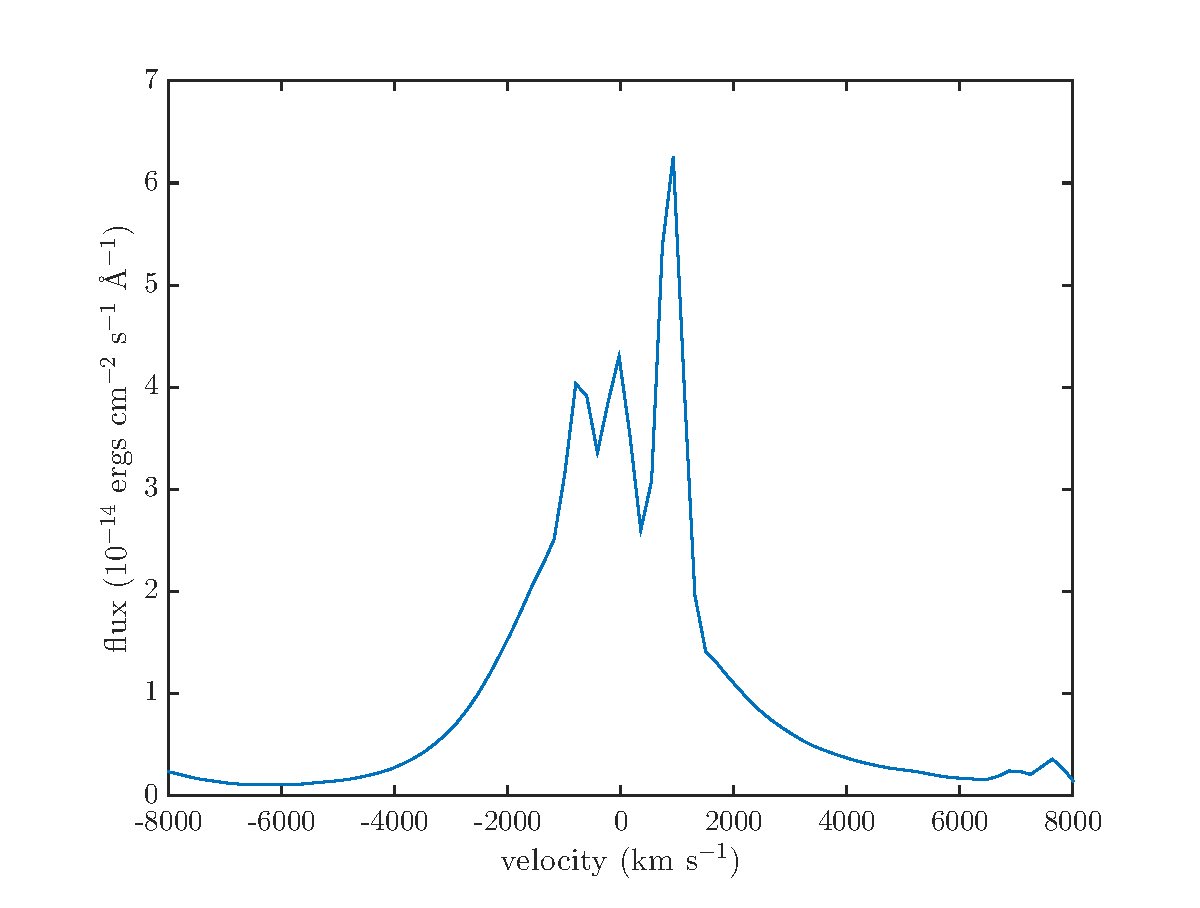
\includegraphics[trim=38 7 35 20,clip=true,scale=0.49]{d1054Ha}
\caption{The H$\alpha$ line at day 1054 showing severe contamination by unresolved nebular lines from the equatorial ring}
\label{d1054}
\end{center}
\end{figure}

 
 By day 1054, all three of the narrow nebular lines are strong.  They remain unresolved in the CTIO data at days 1054 and 1478 and therefore contaminate the entire central region of the H$\alpha$ line profile.  Their presence renders the later two CTIO H$\alpha$ profiles (at days 1054 and 1478) unusable for modelling purposes.  The HST and VLT H$\alpha$ profiles at later epochs ($\ge$ 1862 days) have a higher spectral resolution and it was therefore possible to remove the narrower [N~{\sc ii}] and H$\alpha$ lines from the broad H$\alpha$ profiles (for example Figures \ref{Ha_evol_early} and \ref{Ha_evol_late}). Although this does remove a 
 potentially informative section of the profile ($+500$ km~s$^{-1}<v<+1500$ km~s$^{-1}$), we achieve good fits 
to the overall line profiles at these epochs.




%We postulate however that this feature may in fact be a 
%product of a relatively steep density profile and the formation of dust 
%within the ejecta as demonstrated by both our fits (see Figures 
%\ref{Ha_smooth} and \ref{Ha_clump1}) and our investigation of the parameter 
%space (see Figures \ref{wt} and \ref{bt} ).

%UNCOMMENT FOR THESIS
%It is a general challenge inherent in the nature of this modelling that 
%interesting features that are present in line profiles are not necessarily 
%easily identifiable.  In particular, the effects of clumping and 
%asymmetrical distributions in the ejecta may cause fluctuations that are 
%hard to distinguish from the potential signatures of dust formation 
%discussed in Section \ref{params}.  Key indicators such as symmetry in the 
%location of discontinuities on the red and blue side, typical dust profile 
%signatures and the presence of a red scattering wing should be considered.

%\subsection{Potential challenges at later epochs: days 1862, 2875 and 3604}



%%%%%%%%%%%%%%%%%%%%   SPECTRA   %%%%%%%%%%%%%%%%%%%%%%%%%%%
%%%%%%%%%%%%%%%%%%%%   CODE   %%%%%%%%%%%%%%%%%%%%%%%%%%%
\section{The DAMOCLES code}
\label{code}

Monte Carlo methods have long been used to model radiative transfer 
problems in diverse environments and there are several examples of codes 
which utilise the technique in application to supernovae 
(for example \citet{Maeda2003, Lucy2005c, Jerkstrand2012,Owen2015}).  Whilst there are numerous codes that 
treat dust or gas or both in order to produce an overall spectral energy 
distribution (SED), there is a dearth of codes designed to focus on the 
shapes of inidividual line profiles.  Although a velocity field is naturally 
considered in codes that seek to reproduce the spectra of supernovae, 
absorption and scattering by dust is not and thus the resulting shapes of 
line profiles are potentially unrepresentative of those emerging from 
dusty ejecta at late times.

In this work we aim to model single or doublet line profiles produced by 
a moving atmosphere in a dusty medium.  
Since a comparatively small wavelength range is considered, a fully 
self-consistent radiative transfer model is unnecessarily expensive.  
Instead any energy packet that is absorbed during the simulation may 
simply be removed on the grounds that it would be 
reemitted outside the wavelength range of interest. The extinction due to 
dust is assumed to be temperature-independent and it is therefore 
unnecessary to iteratively calculate the temperature of the ejecta as in a 
fully self-consistent calculation of the SED.  Though clearly the total 
energy transferred through the medium is not conserved in the wavelength range of interest, the signature of 
the normalised line profile is preserved.

The DAMOCLES code builds on the work of \citet{Lucy1989} who employed a 
similar approach to model the broad [O~{\sc i}]~$\lambda$6300,6363~\AA\ doublet 
seen in SN~1987A at early epochs (up to $\sim$ day 775).  It models the 
transport of initially monochromatic energy packets through a smooth or 
clumped dusty medium having a smooth velocity field. The velocity field 
and the inner and outer ejecta radii are free parameters. The late-time 
($> 400$ days) line emission is assumed to be optically thin, with an 
emissivity distribution proportional to the square of the local gas density, i.e. 
proportional to the product of the recombining proton and electron 
densities in the case of H$\alpha$ or to the product of the neutral 
oxygen and electron densities in the case of collisionally excited [O~{\sc 
i}] emission.

\subsection{The energy packet formalism}
\label{packets}

The initial radiation field is inherently tied to the distribution of gas 
throughout the supernova ejecta which is declared as a power law $\rho(r) 
\propto r^{-\beta}$ between $R_{in}$ and $R_{out}$. $R_{out}$ is calculated directly from the epoch of the line to be modelled and the declared maximum line velocity.  The emissivity 
distribution is also specified as a power law with $i(\rho) \propto 
\rho^{k}$.  However this is generally taken to be $i(r) \propto r 
^{-2\beta}$ since the majority of lines modelled are optically thin recombination lines or collisionally excited lines
and therefore $i(\rho) \propto \rho^2$.  The radiation is quantised into 
monochromatic packets with equal energy $E_{0}=nh\nu_{0}$.  In Monte Carlo 
simulations (that model non-moving media) packets are usually taken 
to be of constant energy.  When the frequency of a packet is altered after 
an event, the energy of that packet is kept constant and the number of 
real photons contained within it is assumed to change.  However, in the case 
of dust scattering, the number of real photons is conserved and thus the 
energy of the packet is altered.  This is most easily achieved by 
weighting each packet over all scattering events as 

\begin{equation}
w=\prod_{scat} \frac{\nu'}{\nu}
\end{equation} 

\noindent where $w$ is the weight of the packet and $\nu$ and $\nu'$ are the frequencies of the packet before and after the scattering event respectively.  The final 
energy of each packet is then $E=wE_0$, where $E_0$ is the initial energy 
of the packet.

The supernova ejecta is divided into shells between $R_{in}$ and $R_{out}$ 
and the number of packets to be emitted isotropically in each shell calculated according 
to the emissivity distribution.  For each packet 
a location within that shell and an initial trajectory is randomly sampled 
from an isotropic distribution such that

\begin{align}
\phi&=2\pi\eta \\
 \cos \theta&=2\xi -1
\end{align}

\noindent where $0<\eta<1$ and $0<\xi<1$ are random numbers, $\phi$ is the 
azimuthal angle and $\cos \theta$ is the radial direction cosine.  At 
emission and at each scattering event the frequency of the packet is 
recalculated according to the specified radial velocity field $v(r) 
\propto V_{max}r^{\alpha}$ (see Section \ref{transport}).


\begin{figure*}
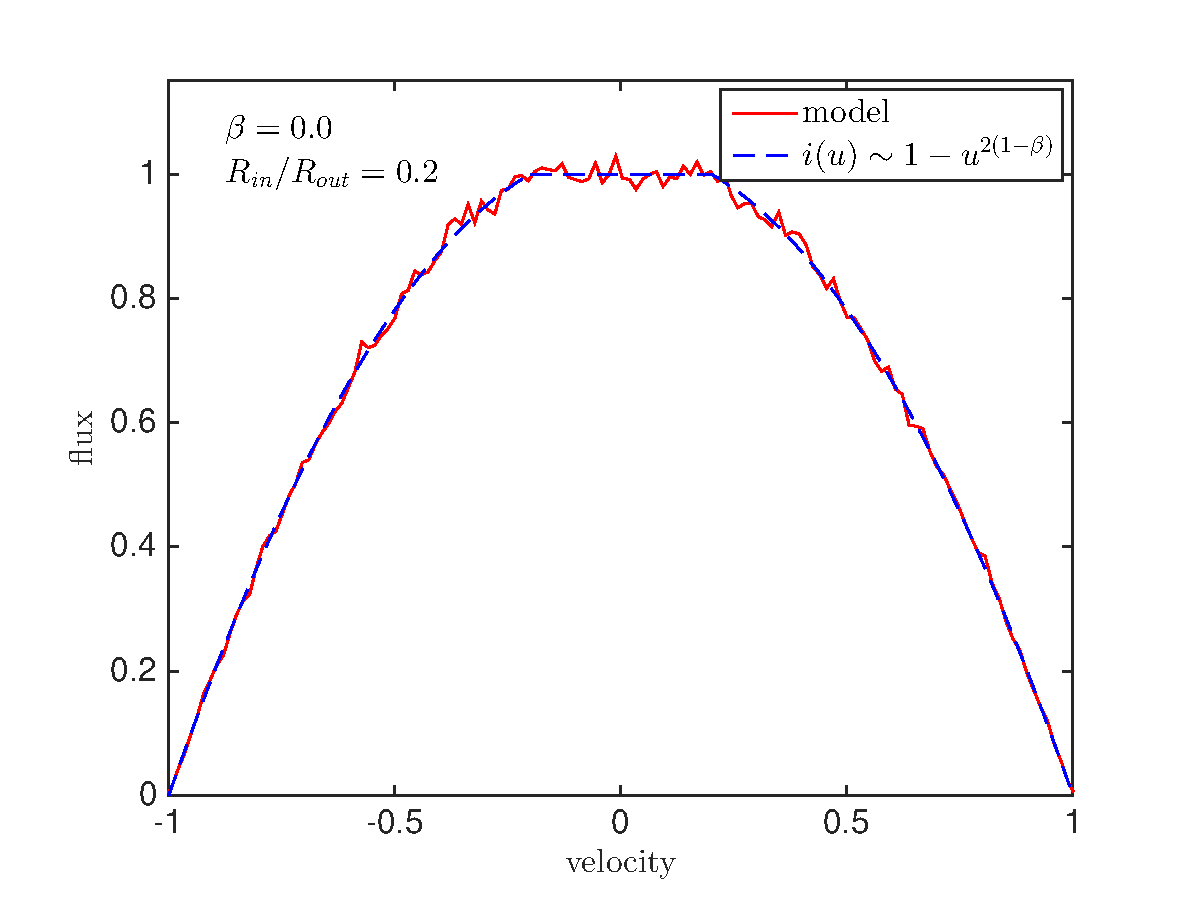
\includegraphics[trim =25 25 45 15,clip=true,scale=0.34]{params/A/b0_r0_2} 
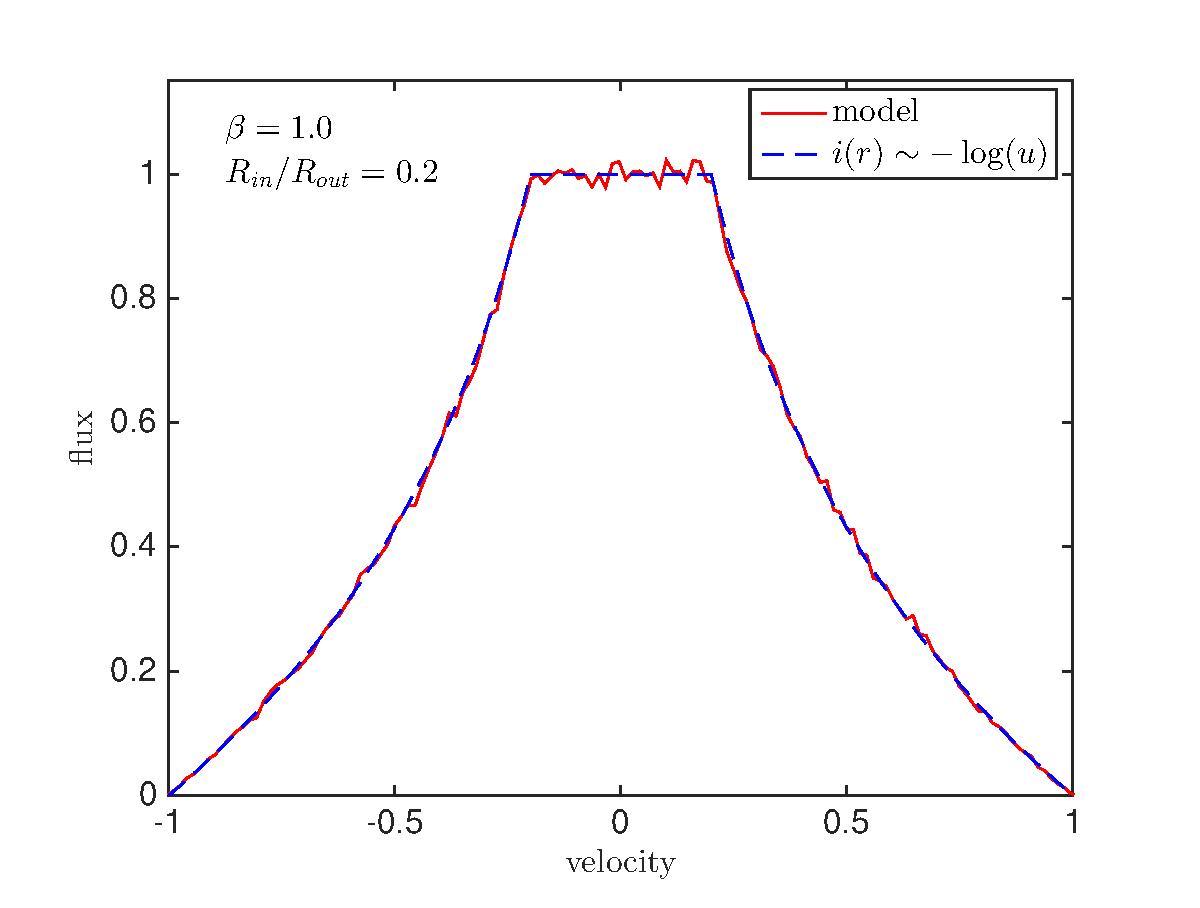
\includegraphics[trim =37 25 45 15,clip=true,scale=0.34]{params/A/b1_r0_2}
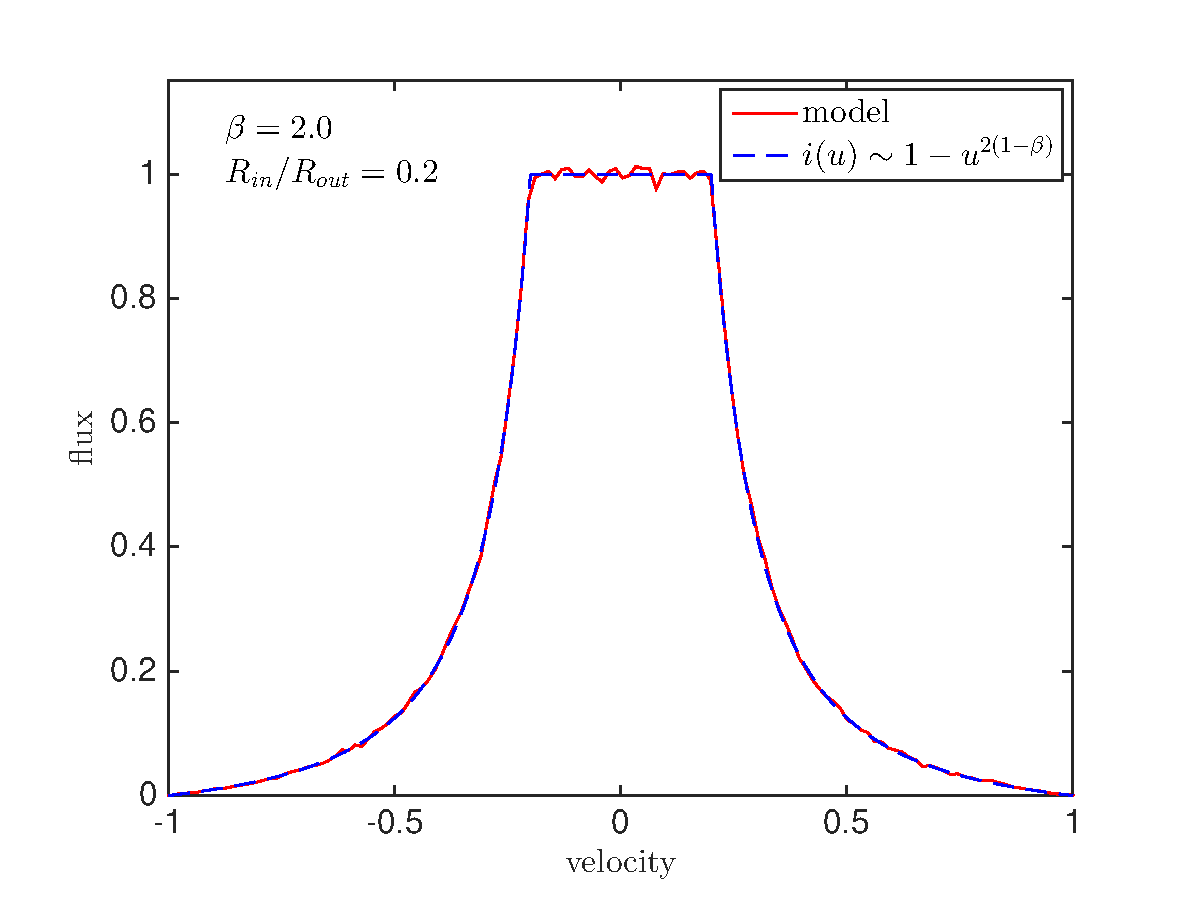
\includegraphics[trim =37 25 45 15,clip=true,scale=0.34]{params/A/b2_r0_2}
\\
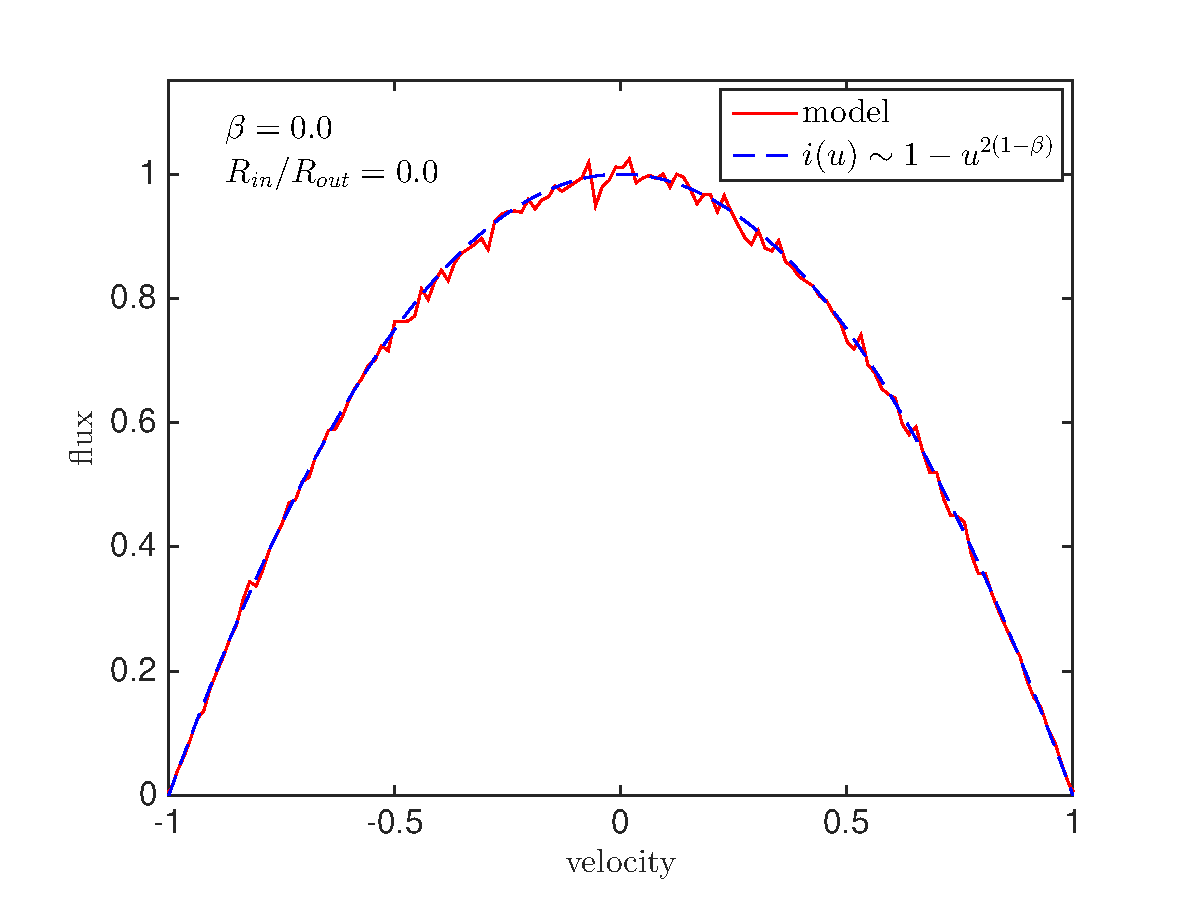
\includegraphics[trim =25 5 45 15,clip=true,scale=0.34]{params/A/b0_r0}  
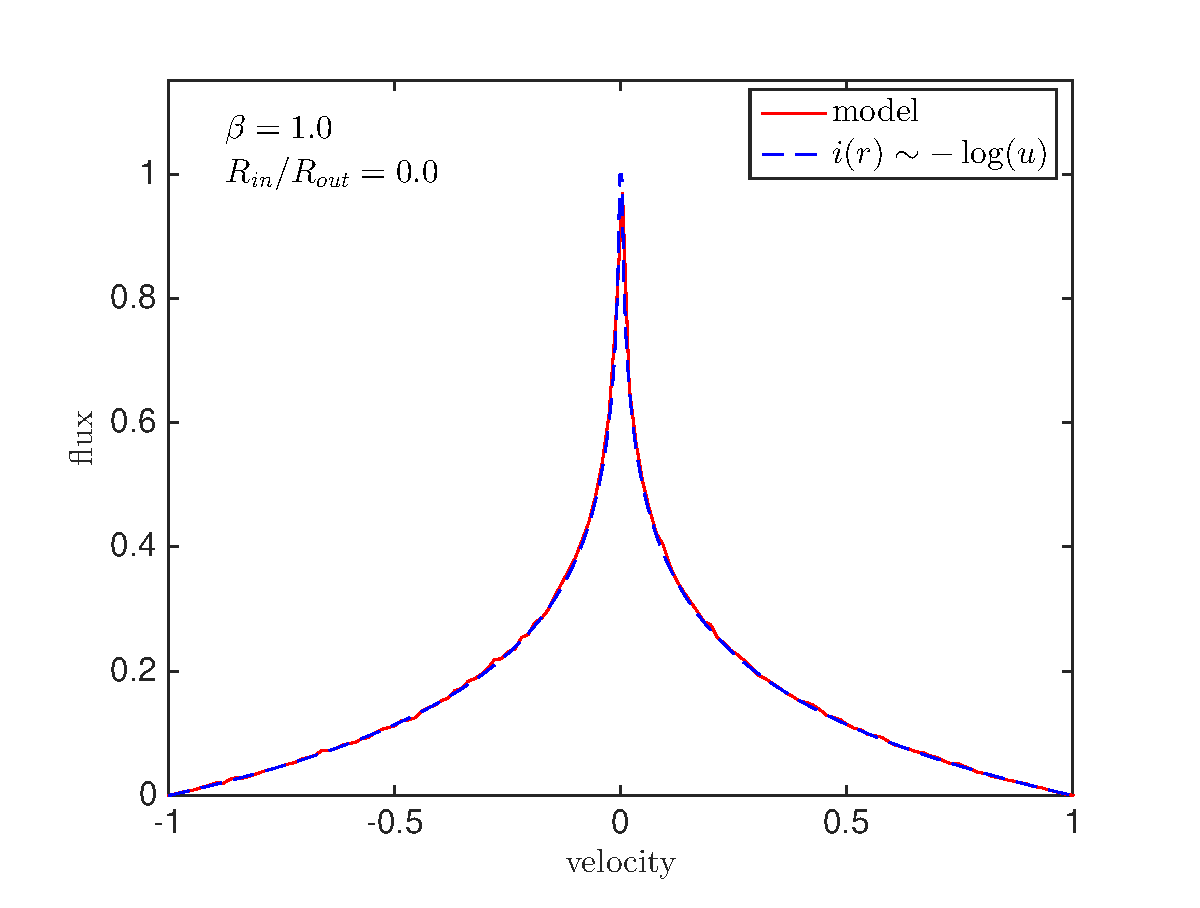
\includegraphics[trim =37 5 45 15,clip=true,scale=0.34]{params/A/b1_r0} 
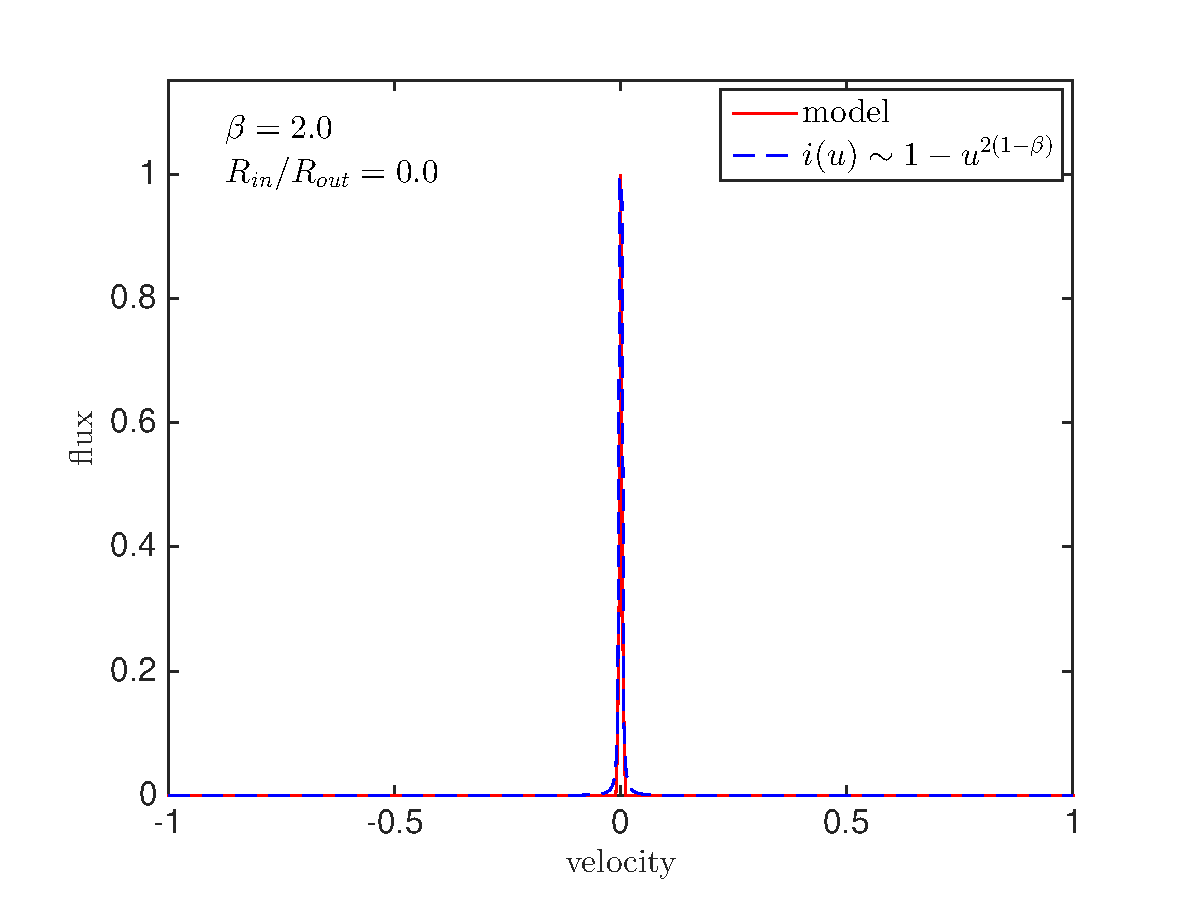
\includegraphics[trim =37 5 45 15,clip=true,scale=0.34]{params/A/b2_r0}

\caption{\textit{Red:} Benchmark models for optically thin ($\tau =0$) 
line profiles  with fractional velocity $v \propto r$. Left to right: initial emissivity 
profiles $i(r) \propto r^{-2\beta}$ with $\beta=0.0$, $\beta=1.0$ and 
$\beta=2.0$. Cases with $R_{in}/R_{out}=0.2$ are on the top and 
with $R_{in}/R_{out}=0.0$ on the bottom.  The presence of a plateau in the upper plots is due to the finite inner radius (detached shell). \textit{Blue:} The analytical case 
with $i(u) \sim 1-u^{2(1-\beta)}$ except in the case of $\beta=1$ where 
$i(u) \sim -\log u$.}
\label{fig:analytics}
\end{figure*}

\subsection{The geometry of the ejecta and the grid}
\label{grid}

The supernova ejecta is approximated by a three-dimensional cartesian 
grid, each cell of which is assumed to have uniform density and 
composition.  The grid is a cube with sides of width $2R_{out}$ and a 
declarable number of divisions.  After the initial emission of energy 
packets, the gas plays no further role in the simulation and thus only 
dust properties are considered.  By default, the dust is coupled to the 
gas (although it may be decoupled) and thus follows the smooth 
distribution described above ($\rho \propto r^{-\beta}$).  The dust 
density in each cell is therefore calculated accordingly and any cell 
whose centre falls outside of the bounds of the supernova ejecta has 
density set to zero.

It is worth noting that if a constant mass loss rate is required, the 
exponent of the velocity profile and the exponent of the density profile 
are not independent.  A constant mass loss rate implies that $4\pi \rho 
vr^2 \propto k$, where $k$ is a constant, and thus for $v \propto 
r^\alpha$ and $\rho\propto r^{-\beta}$, we require that $\beta-\alpha=2$.  
However, it is possible that the supernova event may have induced a 
mass-flow rate that is not constant with radius and thus both exponents 
may be declared independently.

It is known from SED modelling that clumped environments produce very 
different results to environments assumed to have a smooth distribution of 
dust and gas.  Specifically, clumped models tend to require a higher dust mass in 
order to reproduce a similar level of infrared dust emission compared to a smoothly distributed model.  The 
capacity for modelling a clumped dusty medium is therefore included in the 
code.  The fraction of the dust mass that is in clumps is declared 
($m_{frac}$) and the total volume filling factor of the clumps ($f$) is 
also specified.  Dust that is not located in clumps is distributed 
according to a smooth radial profile.  The clumps occupy a single grid 
cell and their size can therefore be varied by altering the number of 
divisions in the grid.  The clumps are distributed stochastically with the 
probability of a given cell being a clump proportional to the smooth 
density profile (i.e. $p(r) \propto r^{-\beta}$).  The density within all 
clumps is constant and is calculated as

\begin{equation}
\rho_{clump}=\frac{M_{clumps}}{V_{clumps}}=\frac{m_{frac}M_{tot}}{\frac{4}{3} f\pi (R_{out}^{3}-R_{in}^{3} )}
\end{equation}

\noindent where $M_{tot}$ is the total dust mass, $M_{clumps}$ is the 
total dust mass in clumps and $V_{clumps}$ is the total volume occupied by 
clumps.  $m_{frac}$ and $f$ are defined as above.


\subsection{The radiative transport mechanism}
\label{transport}

Following emission, a packet must be propagated through the grid until it 
escapes the outer bound of the ejecta at $R_{out}$.  The probability that the 
packet travels a distance $l$ without interacting is $p(l)=e ^{-n \sigma 
l}=e ^{-\tau} $ where $n$ is the grain number density, $\sigma$ is the 
cross-section for interaction and $ \tau = n\sigma l$ for constant $n$ and 
$\sigma$ (as in a grid cell).  Noting that the probability that a packet 
will interact within a distance $l$ is $1-e^{-\tau}$, we may 
sample from the cumulative probability distribution to give:

\begin{align}
\xi = 1 - e^{-\tau} \implies \tau= -\ln (1-\xi)
\end{align}

\noindent where $0<\xi<1$ is a  random number sampled from a uniform distribution.
% representing the probability of interaction within $\tau$.  
The frequency of the 
photon packet and the mass density of the cell are then used to calculate 
the opacity of that cell. Using the fact that $n\sigma=\kappa\rho$, 
the distance $l$ that the packet travels before its next interaction is 
calculated.  If this value is greater than the distance from its position 
to the edge of the cell then the packet is moved along its current 
trajectory to the cell boundary and the process is repeated.  If the 
distance is less than the distance to the boundary then an event occurs 
and the packet is either scattered or absorbed, with the probability of 
scattering equal to the albedo of the cell

\begin{equation}
	\omega=\frac{\sigma_{sca}}{\sigma_{sca}+\sigma_{abs}}
\end{equation}

If the packet is absorbed then it is simply removed from the simulation as 
discussed above.  If the packet is scattered then a new trajectory is 
sampled from an isotropic distribution in the comoving frame of the dust 
grain and the frequency of the packet is recalculated using Lorentz 
transforms subject to the velocity at the radius of the interaction (see 
Appendix A for further details).  This process is repeated until the 
packet has either escaped the outer boundary of the supernova ejecta or has been 
absorbed.
   
Escaped photon packets are added to frequency bins, weighted by $w$, in order to 
produce an overall emergent line profile.


\subsection{Properties of the Dusty Medium}

Dust of any composition for which optical data are available may be used
and the relative abundances of the species may be declared by the user.  
A grain size may be specified for each species.  Since a full radiative 
transfer calculation is not performed, it is not useful to specify a grain 
size distribution since the extinction due to dust is only dependent on the 
cross-sectional area of the grains and not on the overall distribution.  
The capacity to declare a size distribution is however included for the 
sake of ease of comparison with SED models.  Mie theory and optical properties are used 
to calculate the overall $Q_{abs}(\nu)$ and $Q_{sca}(\nu)$ for each 
species and the derived opacities are summed over each species weighted 
according to their relative abundances.


As will be discussed in Section \ref{params}, the effects of scattering 
on the shapes of line profiles can potentially be quite pronounced and it 
is therefore important to consider the potential effects of electron 
scattering as well as those of dust scattering.  Electron densities are 
calculated using an estimated average temperature of 10,000K and the observed luminosity 
of H${\alpha}$ and the optical depth to electron scattering calculated from this.  
Electron scattering is treated in an identical manner to dust scattering, 
with $\tau = \tau_{dust}+\tau_{e}$ in each cell.  If, for a given 
packet, an event occurs, it is first calculated whether this is an electron scattering event or a dust 
event (either scattering or absorption) by considering the ratio of the optical depths to each.  If the packet is scattered by an electron then the velocity of that electron is calculated by considering the bulk velocity at that radius and adding a thermal velocity component following the formalism described by \citet{Hillier1991}.  The scattering 
process is then identical to that for dust.  If the event is a dust event then the process continues as described above.

In the majority of cases the electron scattering optical depths are not high 
enough to discernibly affect the overall shape of the profile.  However, 
there may be some early epoch cases (the concept is discussed for SN 2010jl 
by \citet{Fransson2014}) where the electron scattering optical depths are high enough to 
become significant in the observed profiles.  

\begin{figure*}
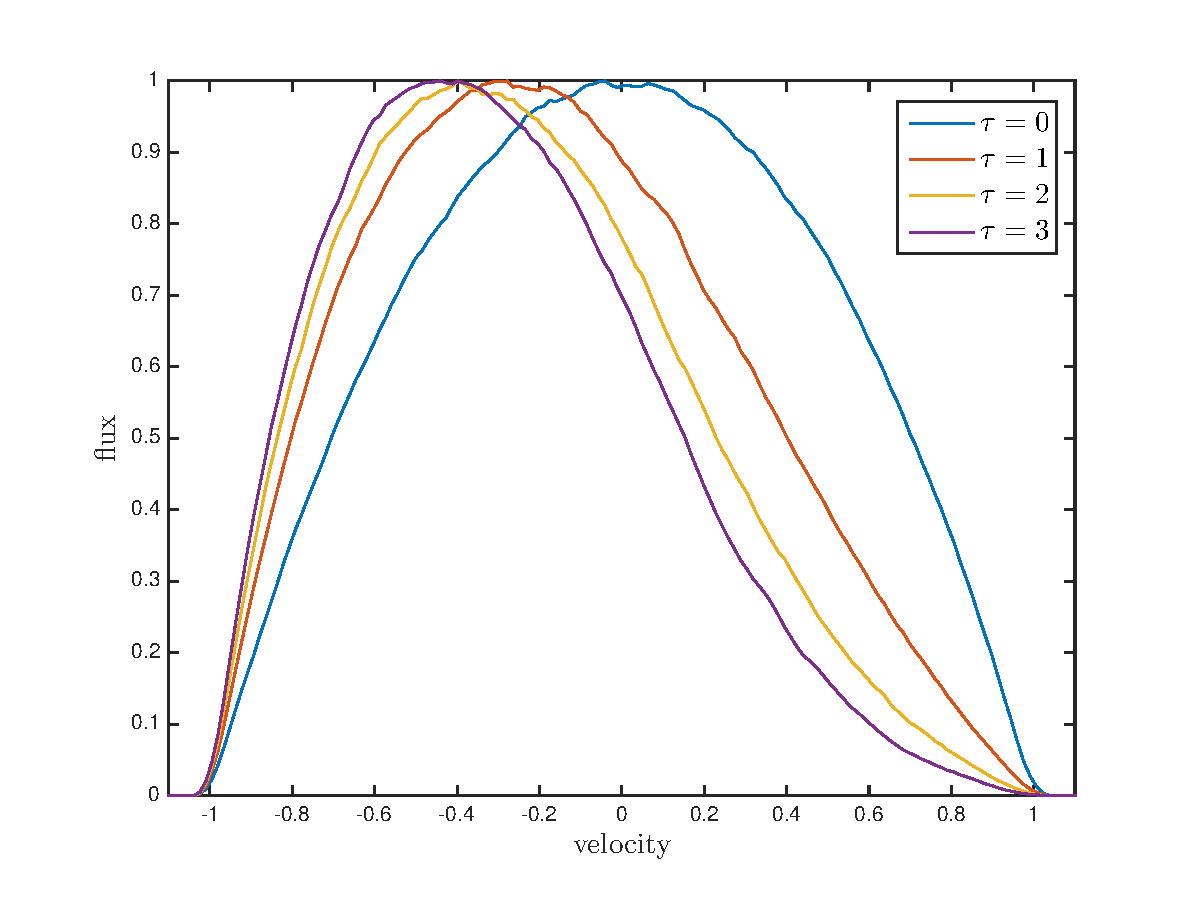
\includegraphics[trim =33 10 45 15,clip=true,scale=0.51]{params/opt_thick_w0} 
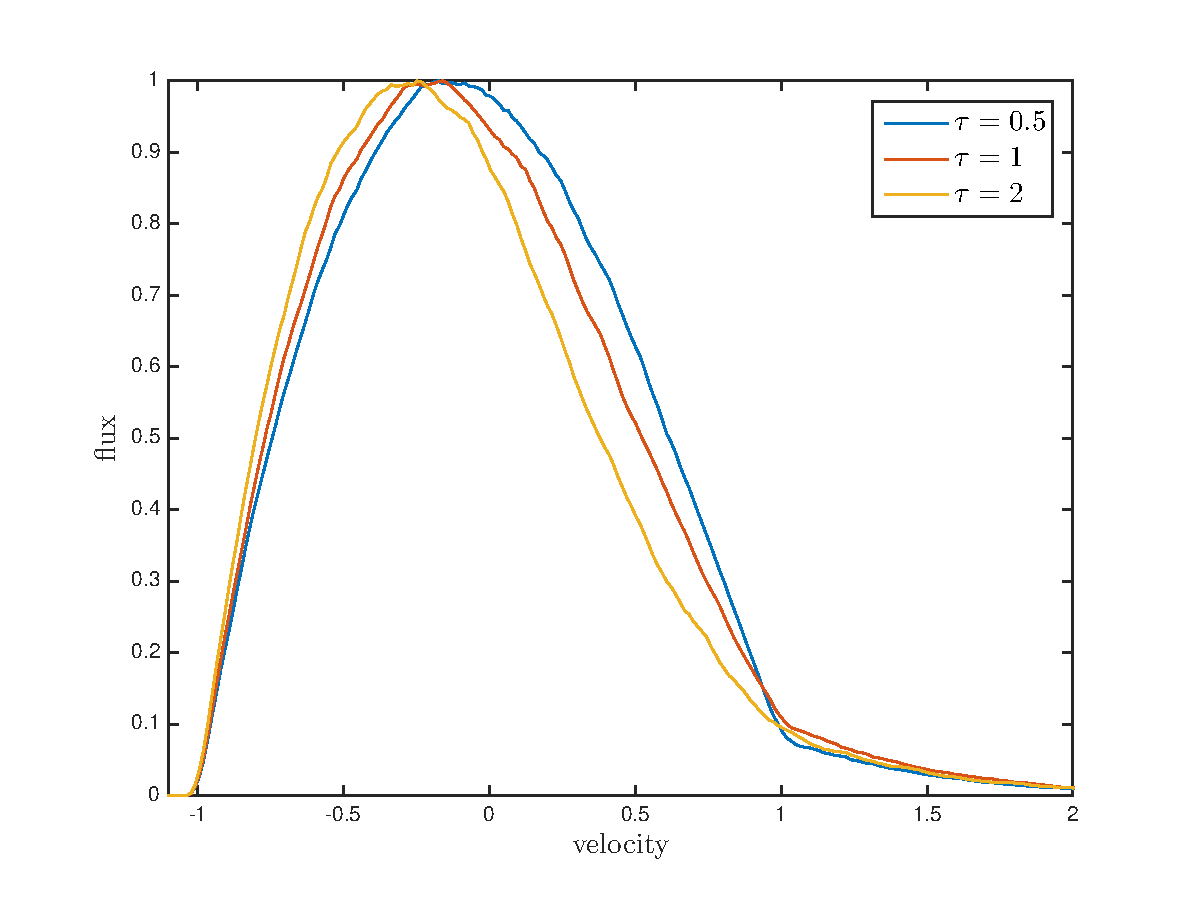
\includegraphics[trim =33 10 45 15,clip=true,scale=0.51]{params/opt_thick_w0_6}  
\caption{Benchmark models for line profiles  with $v \propto r$, $i(r) \propto$ constant and a filled sphere with $R_{in}/R_{out}=0$.  Pure dust absorption models ($\omega = 0$) are presented in the left-hand plots, whilst partially scattering models are presented on the right ($\omega = 0.6$) as per \citet{Lucy1989} Models II and III. All resulting profiles have been scaled to unit flux at their peaks.}
\label{fig:Lucy}
\end{figure*}
%%%%%%%%%%%%%%%%%%%%   CODE   %%%%%%%%%%%%%%%%%%%%%%%%%%%



%%%%%%%%%%%%%%%%%%%%   TESTING/PARAMS   %%%%%%%%%%%%%%%%%%%%%%%%%%%
\section{Comparison of DAMOCLES models with analytical and previously published results}
\label{params}

There is a general lack of published models in the literature that 
consider dust absorption-affected asymmetric line profiles.  We therefore test 
the code by comparing the results to optically thin profiles that may be 
derived analytically.  We then test the absorption and scattering 
components of the code by comparing our results for the case of an 
optically thick medium with those derived by \citet{Lucy1989} in their 
Model II and Model III scenarios.

\subsection{Comparison of DAMOCLES models with analytical results}
\label{analytics}

Analytical profiles may be calculated in the dust-free case.  We ran a 
number of models based on the methods of \cite{Gerasimovic1933} 
who derived equations for line profiles emitted from a transparent 
expanding shell.

Describing the fractional expansion velocity of the shell as $v(r) \propto r^\alpha$ with 
$\alpha \neq 0$ such that $v(r)=\frac{V(r)}{V_{max}}$ where $V(r)$ and $V_{max}$ represent physical velocities and $v_{max}=1$, the energy emitted by 
the nebula between radial velocities $v$ and $v+dv$ is proportional to

\begin{equation}
\int _\tau i(r) r \sin (\theta) \, r \, d\theta \, dr
\end{equation}

\noindent where $i(r)$ represents the emission per unit volume at radius 
$r$ and $\theta$ is the angle to the observer's line of sight.  We adopt inner radius $R_{in}=q$  and outer radius $R_{out}=1$ such that $q=R_{in}/R_{out}$.


Setting $i(r) \propto r^{-2\beta}$ (for a recombination or collisionally excited line emitted from 
a medium with an assumed density profile for the emitter $\rho \propto 
r^{-\beta}$) then gives

\begin{equation}
\begin{split}
i(v) \, dv &\sim \frac{dv}{\alpha v^{\frac{2\beta-3+\alpha}{\alpha}}} \int^{\theta_1}_{\theta_0} \cos^{\frac{2\beta-3}{\alpha}} \theta \sin \theta \, d\theta 
\\
&\sim  \frac{dv}{v^{\frac{2\beta-3+\alpha}{\alpha}}} \Bigg[\frac{\cos^{\frac{2\beta - 3 + \alpha}{\alpha}} \theta}{2\beta -3 + \alpha}\Bigg]^{\theta_1}_{\theta_0}
\end{split}
\end{equation}

\noindent for $\frac{2\beta-3}{\alpha} \neq -1$ where $i(v) \,dv$ is the energy emitted in a volume element and $\theta_0$ and $\theta_1$ are the bounds of this element.  The case 
$\frac{2\beta-3}{\alpha} = -1$ results in a logarithmic relationship.


In the case of a ``filled'' nebula, i.e. one where the inner radius is 
vanishingly small in comparison to the outer radius, we obtain

\begin{equation}
\label{eqn:sides}
	i(v) \, dv \sim \pm \frac{du}{(2\beta-3+\alpha) v^{\frac{2\beta-1+\alpha}{\alpha}}} \Big(1-v^{\frac{2\beta-3+\alpha}{\alpha}} \Big)
\end{equation}

If the nebula is not ``filled'', that is to say, the inner radius is some fraction of the outer radius and the remnant is a detached shell, the above formula becomes valid only from $v=1$ to some critical value $v'=q^\alpha$. For $v<v'$, we obtain

\begin{equation}
i(v) \, dv \sim \pm \frac{dv}{(2\beta-3+\alpha)} \Big( \frac{1}{q^\alpha} - 1 \Big)
\end{equation}

\noindent and therefore the top of the line is flat while the sides are 
sloping.

Crucially, the width of the flat section is determined by $v'=q^\alpha$ or 
simply $v'=q$ in the case where $v \propto r$, whilst the shape of the 
profile outside of the flat top is described by equation \ref{eqn:sides}.

Profiles with a variety of shapes may be derived from these formulae 
depending on the relative values of $\alpha$ and $\beta$.  Here we 
consider three main families of curves:


%\begin{minipage}{0.55\textwidth}
\begin{enumerate}\parskip3pt

	\item \ \ $\quad i(v)  \sim v^{-\gamma}-1$ \quad ($\alpha>0$, $2\beta-3+\alpha>0$)
	\item \ $\quad i(v)  \sim 1-v^\gamma$ \quad \ \ ($\alpha>0$, $2\beta-3+\alpha<0$)
	\item  $\quad i(v) \sim -\log v$ \quad \ \ ($\alpha>0$, $2\beta-3+\alpha=0$)

\end{enumerate}
%\end{minipage}


\noindent where $\gamma$ is defined as $\gamma= \lvert 
\frac{2\beta-3+\alpha}{\alpha} \rvert$.

Models are presented for each of these cases, both for a 
filled nebula and for a shell structure with $R_{in}/R_{out}=0.2$.  
A velocity profile $v \propto r$ appropriate for supernova ejecta in the free 
expansion phase is used throughout \citep{Li1992,Xu1992,McCray1996,Baron2005}.  Values of $\beta = 0, 1$ and $2$ are 
adopted.  Figure \ref{fig:analytics} illustrates the excellent agreement between 
the analytical case and the models.  All fluxes are scaled to unity at the peak.

\subsection{Comparison of DAMOCLES models with previously published results}
\label{opt_thick_testing}



In addition to the tests for optically thin lines described above, we also 
compared our outputs to those derived by \citet{Lucy1989} in order to 
assess the accuracy of the scattering and absorption aspects of the code.  
We consider two similar cases, equivalent to Models II and III of 
\citet{Lucy1989}. In the first case, dust with zero albedo (pure absorption) is 
uniformly distributed throughout a filled nebula with a velocity profile 
$v \propto r$.  In the second case, the same scenario is considered but a 
medium of dust with albedo $\omega =0.6$ is considered.

\begin{figure*}
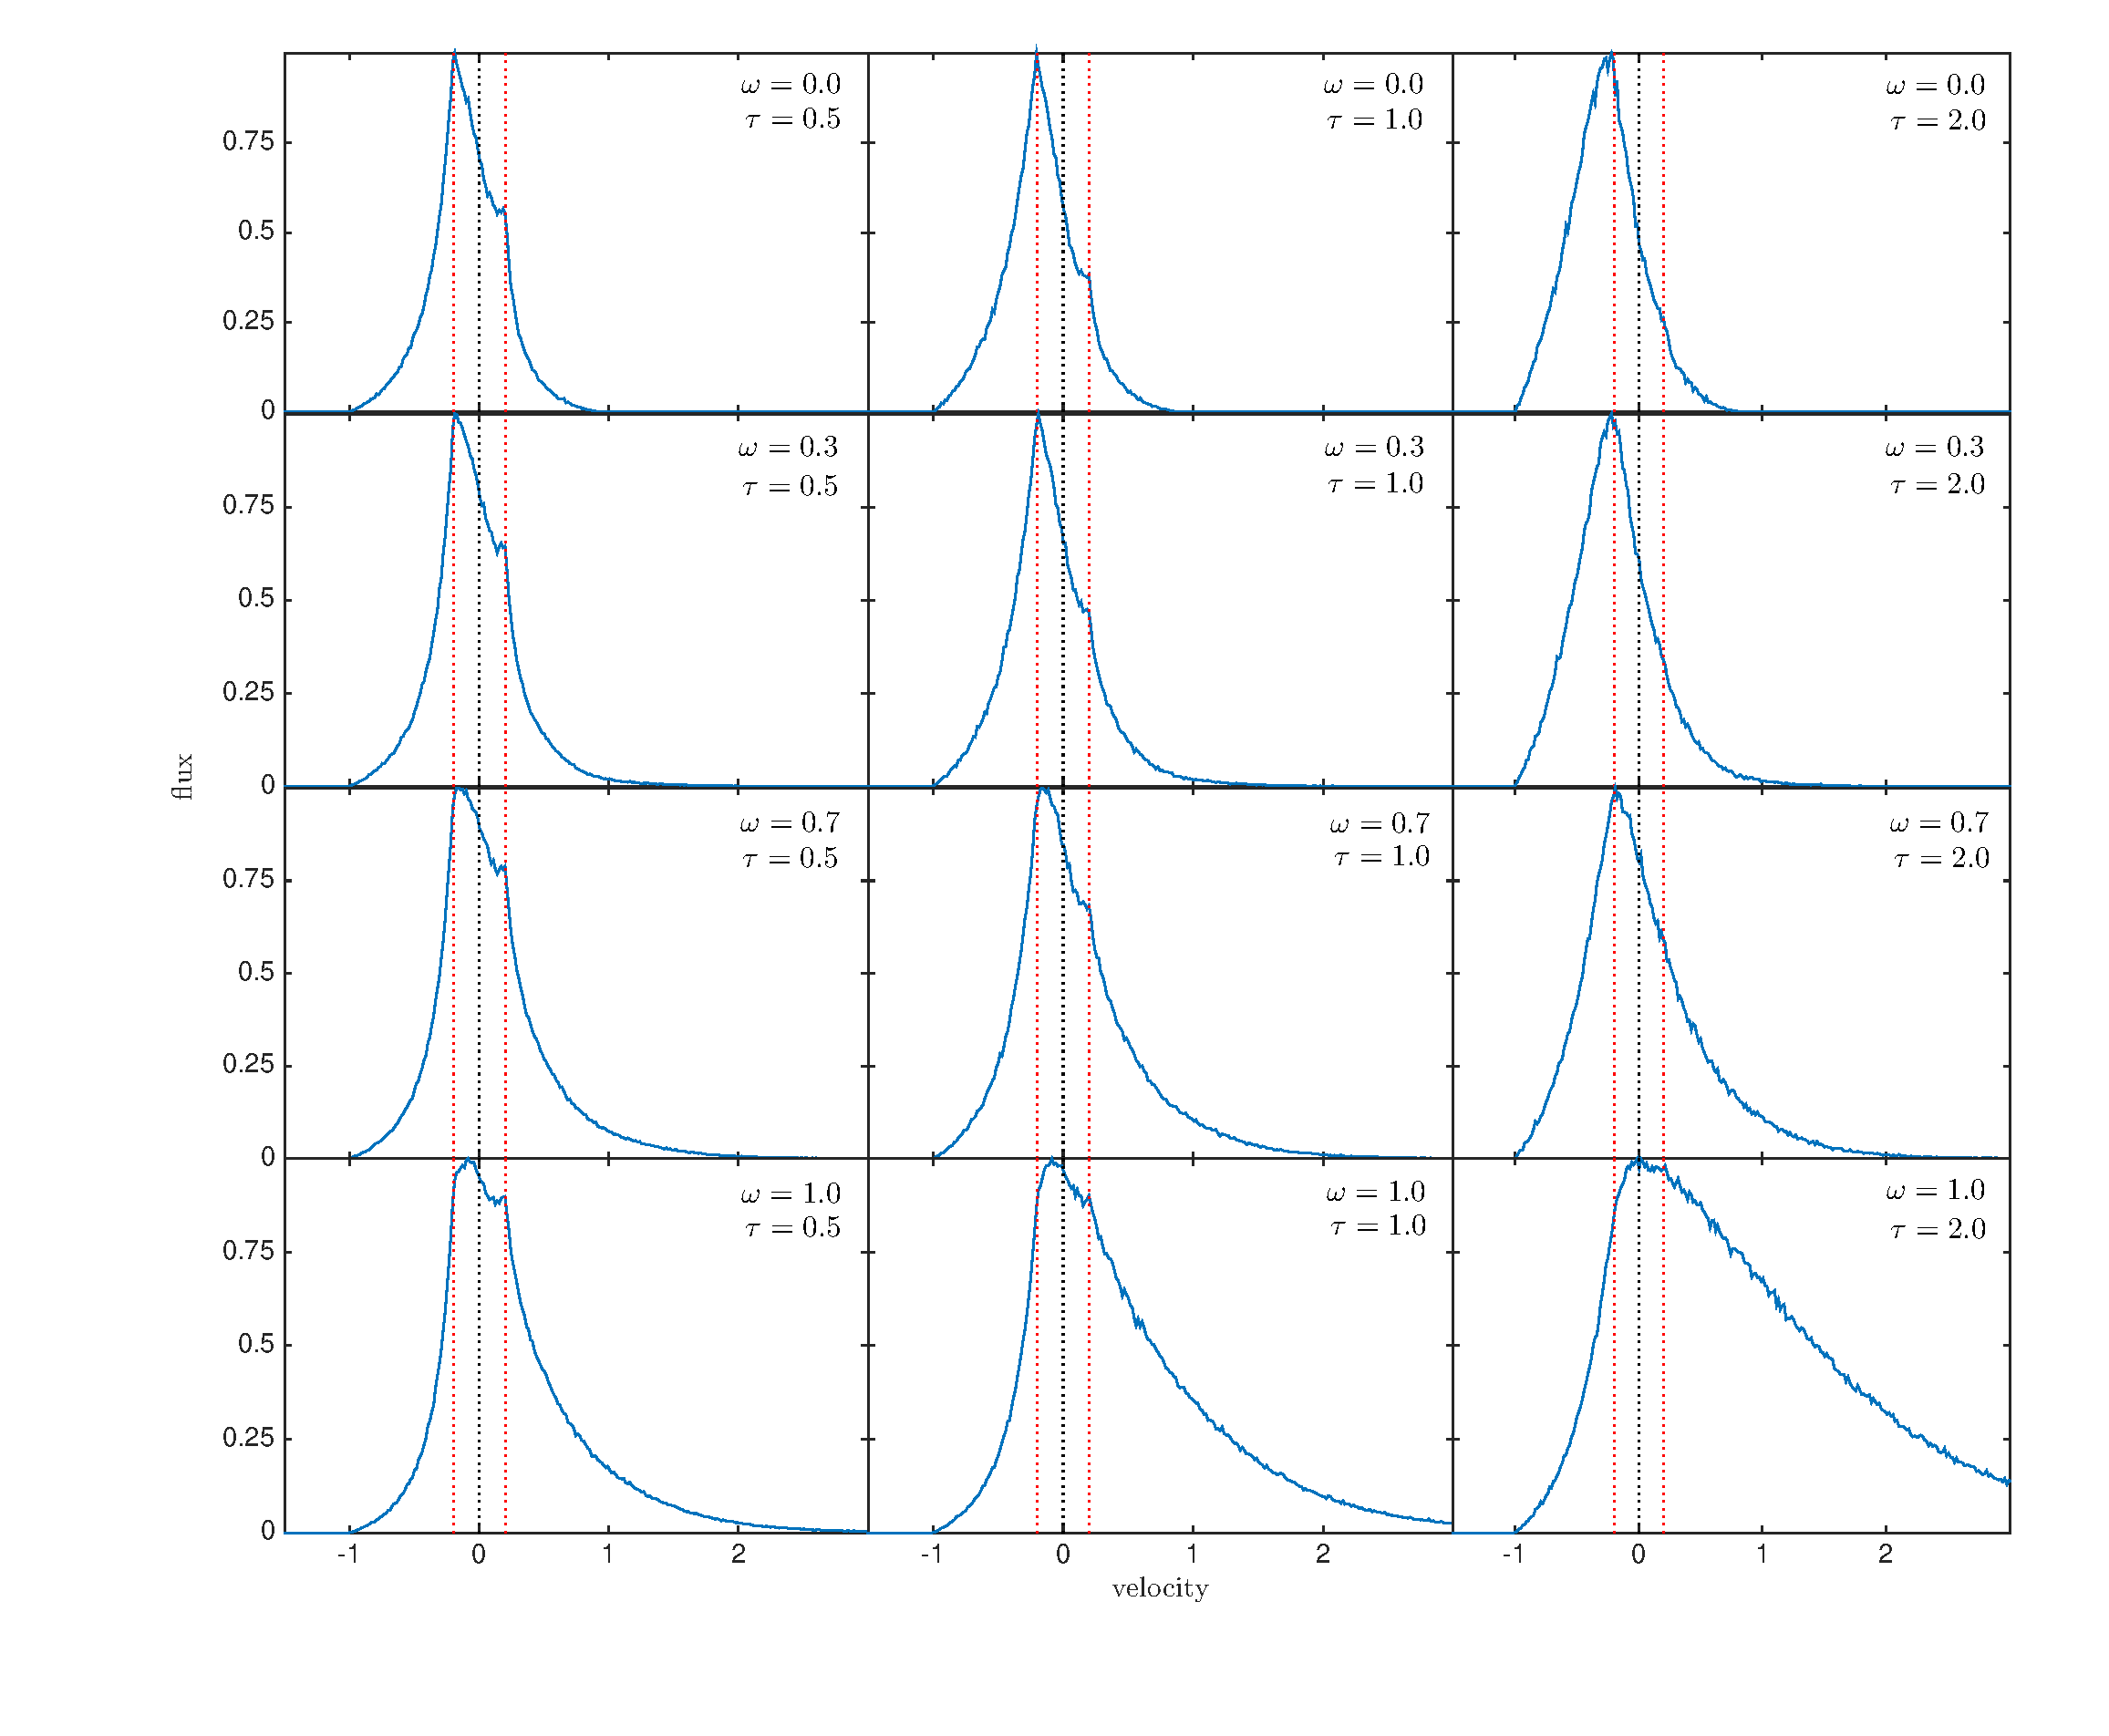
\includegraphics[trim =80 10 40 15,clip=true,scale=0.515]{params/C/C_all} 
\caption{Set of models with $i(r) \propto r^{-4}$ (i.e. $\beta=2.0$), $R_{in}/R_{out}=0.2$, $v(r) \propto r$  
and $v_{max}=1$ illustrating the effects of varying the dust optical depth $\tau$ and albedo $\omega$. 
Peak fluxes are scaled to unity.}
\label{wt}
\end{figure*}


In the first case, the profile may once again be derived analytically from 
the basic geometry using the fact that radiation will be attenuated by a 
factor $e^{-2\tau_{\nu} v}$ between points with line of sight fractional velocities $-v$ and 
$+v$ where $\tau_{\nu}$ is the optical depth at frequency $\nu$ from the centre to the outer edge of the ejecta.  The line profile is therefore given by

\begin{equation}
\frac{I(v)}{I(-v)} = \exp(-2\tau_{\nu} v)  
\end{equation}

\citet{Lucy1989} presented several examples for both the analytical case of 
the perfect absorber and a Monte Carlo model for grains with $\omega 
=0.6$.  We present the same cases in Figure \ref{fig:Lucy} and note that 
the resulting profiles exhibit the same features and shape. Of particular 
interest is the scattering wing that appears beyond the maximum velocity 
($v_{max}=1$) on the red side of profiles in the partial 
scatterer case as a result of the packets doing work on the expanding sphere.  
This was noted by \citet{Lucy1989} as a potential diagnostic for the 
presence of dust in the ejecta of a supernova and we will discuss this 
further in Section \ref{ps}.


\subsection{The sensitivity of the variable parameters}
\label{ps}


\begin{figure*}
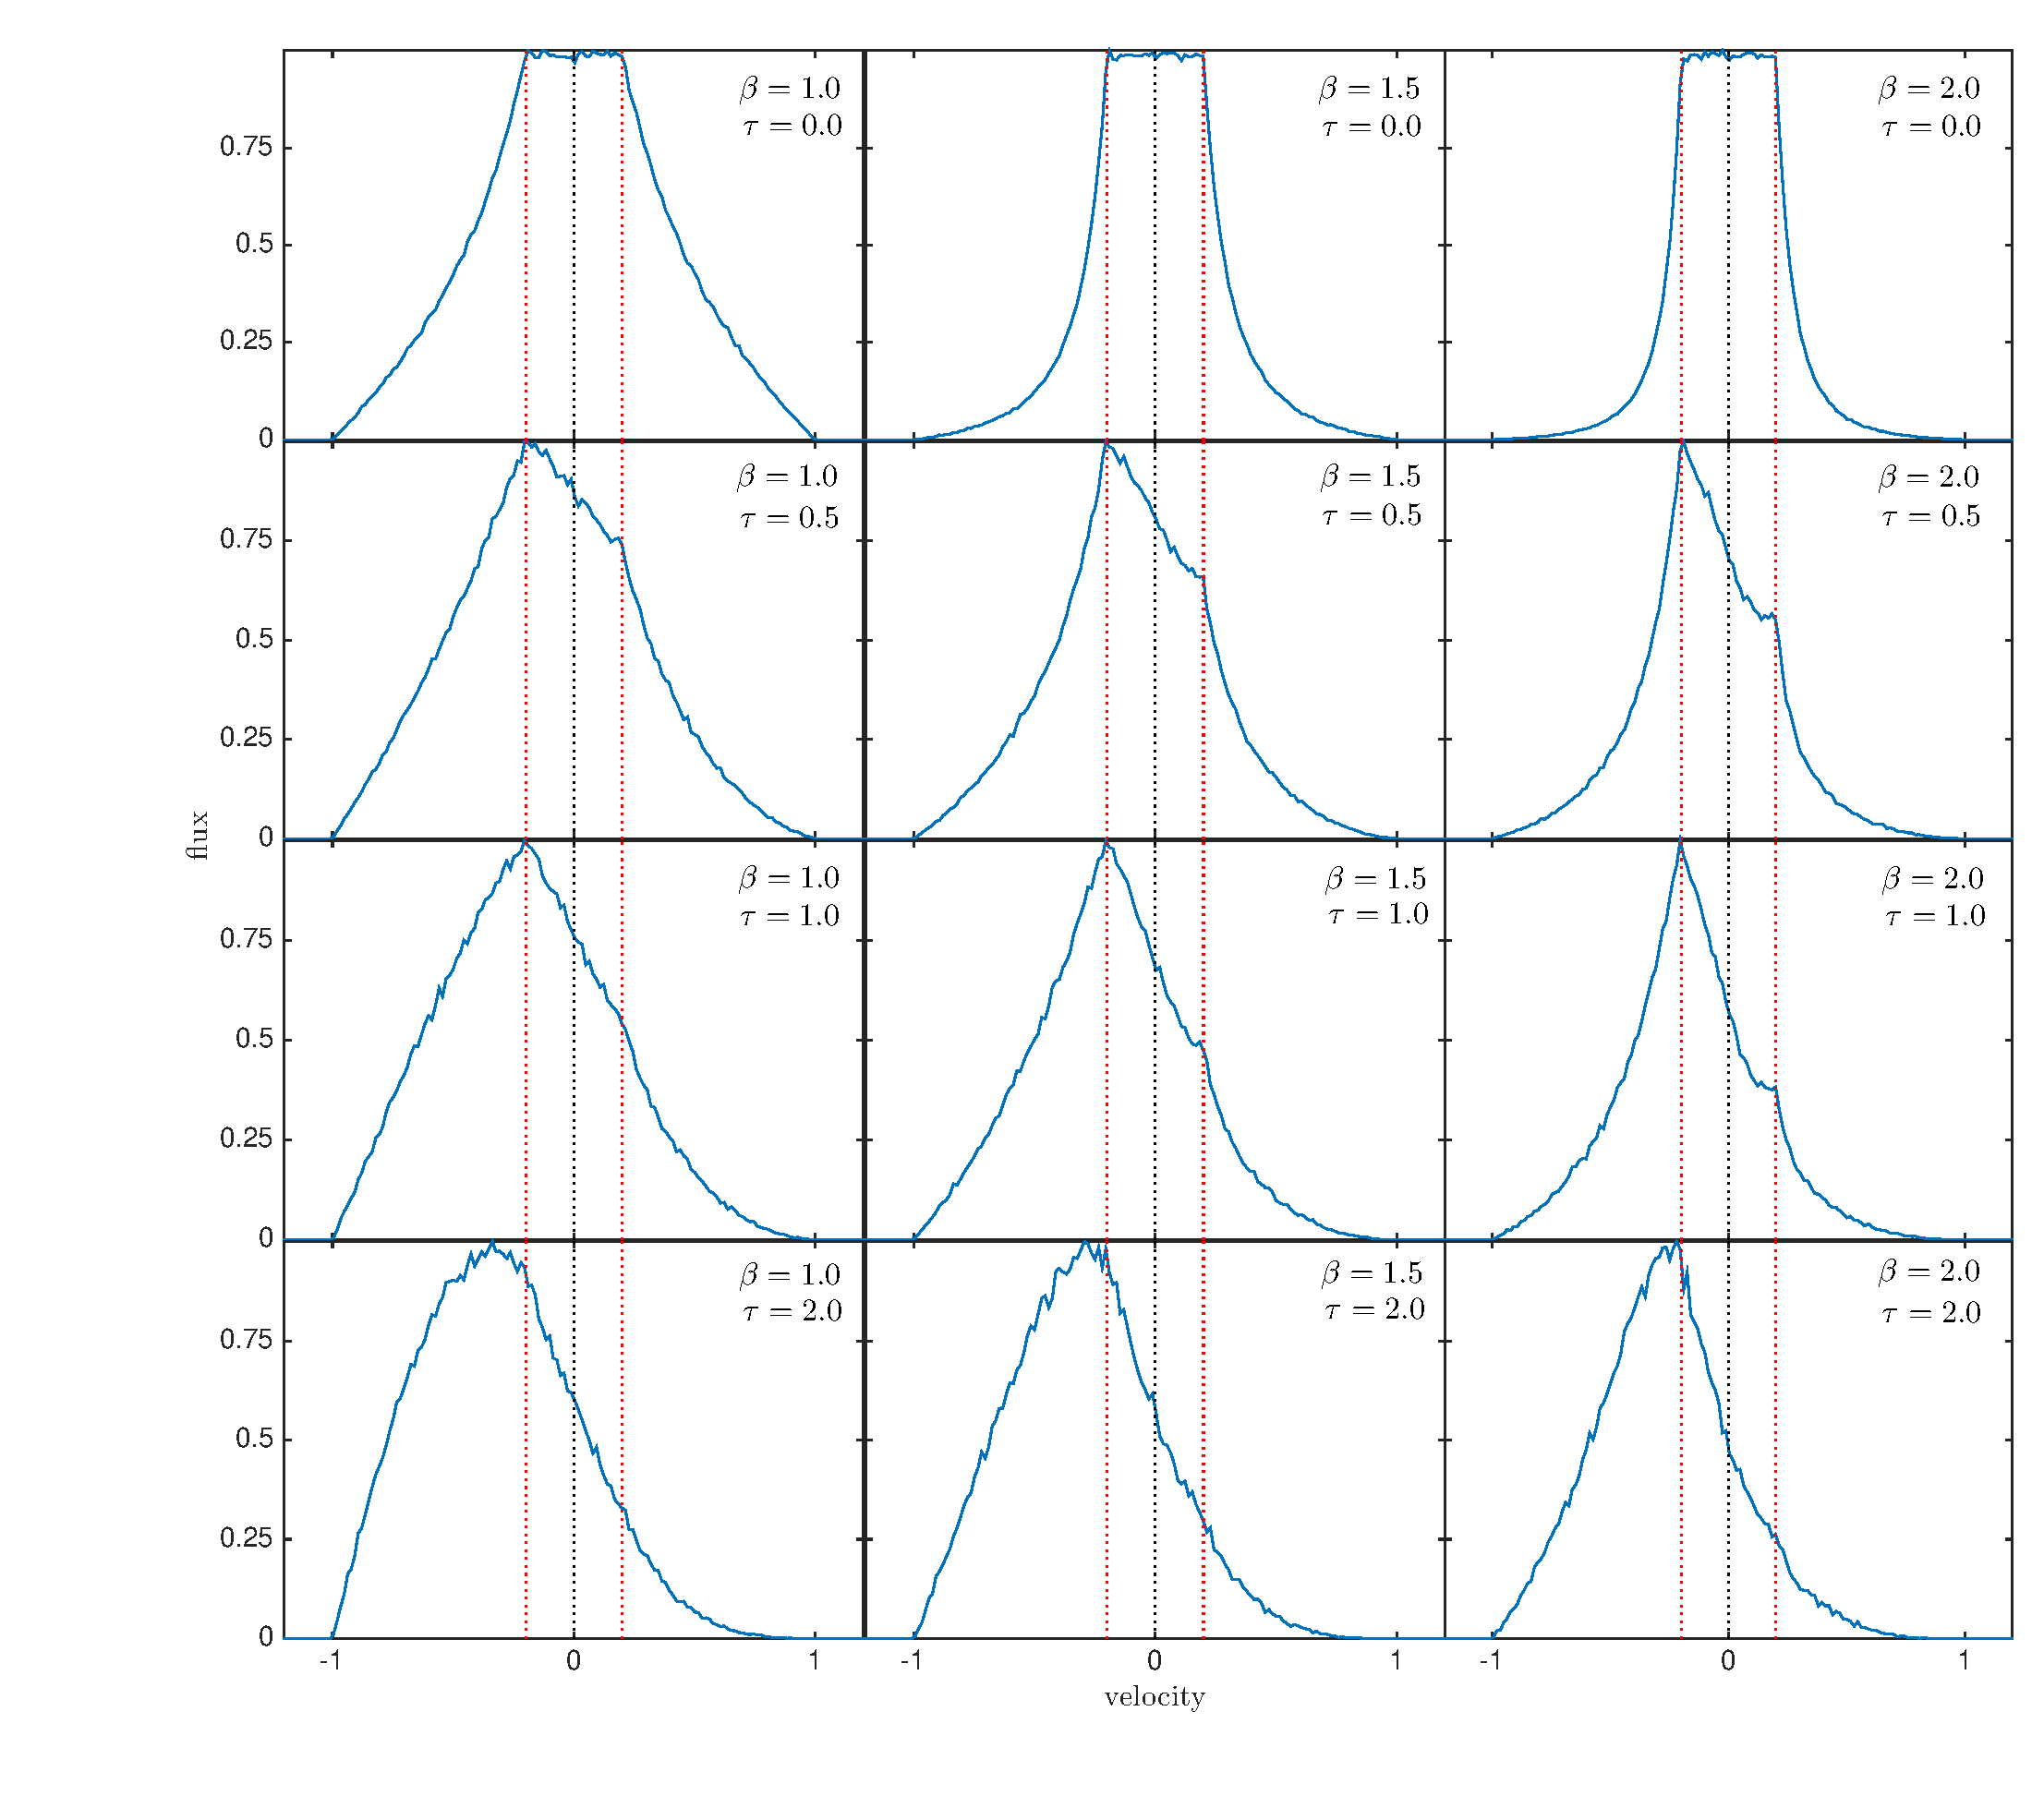
\includegraphics[trim =80 10 6 15,clip=true,scale=0.515]{params/D/newDall} 
\caption{Set of models with $i(r) \propto r^{-2\beta}$ for $\beta=1.0$ \textit{(left)}, $\beta=1.5$ (middle) or $\beta=2.0$ \textit{(right)}, $\omega=0$, 
$R_{in}/R_{out}=0.2$, $v(r) \propto r$ and $v_{max}=1$ illustrating the effects of varying 
the dust optical depth $\tau$.  Peak fluxes are scaled to unity.}
\label{bt}
\end{figure*}


It is of general interest to establish potential diagnostic signatures in 
the line profiles of supernovae and their remnants in order to trace dust 
formation more effectively.  We here discuss the effects of the main 
parameters of interest, namely:

\begin{itemize}
\item the maximum line velocity $V_{max}$
\item the ejecta radius ratio  $R_{in}/R_{out}$
\item the dust optical depth $\tau$
\item the dust albedo $\omega$ 
\item the density profile index $\beta$, where $\rho \propto r^{-\beta}$
\end{itemize}


\subsubsection{The maximum line velocity $V_{max}$}

The maximum velocity is defined as the velocity at the outer edges of 
the line emitting region for a given line.  The 
maximum velocity may vary between different spectral lines or doublets due 
to different locations of  species having differing ionization 
thresholds.  Clearly, the larger the maximum velocity used the wider the 
profile becomes.  To some extent therefore the steepness of the density 
profile and the maximum velocity can act to counter each other since a steeper 
density distribution narrows the profile (see Section \ref{beta}).  The shape 
of the wings of the profiles, however, generally preclude much degeneracy 
in this aspect - the overall shape of the line profile can be used to determine the 
exponent of the density distribution to within a relatively small range.

More important is the effect that the maximum velocity has on the overall 
optical depth.  Since the outer radius is calculated directly from the maximum velocity, the overall volume of the ejecta is determined 
solely by the this value and the ratio of the inner and outer radii.  
The total dust optical depth to which the radiation is exposed can therefore be greatly affected by even a relatively small change in the maximum velocity for fixed values of the other parameters.  
Practically, however, the maximum velocity can usually be fairly well determined 
from the observations (identified as the point where the flux vanishes 
on the blue side) and may be further constrained through modelling.

\subsubsection{The ejecta radius ratio $R_{in}/R_{out}$}

As already discussed in Section \ref{analytics}, the width of the flat top 
is determined by the ratio of the inner and outer radii, the 
exponent of the velocity profile and the maximum velocity.  We 
assume that the velocity profile takes the form $v \propto r$ from 
just a few months after the explosion as the supernova is in free 
expansion.  For this case, $R_{in}/R_{out}$ is given by

\begin{equation}
\frac{R_{in}}{R_{out}}=\frac{V_{min}}{V_{max}}
\end{equation}

\noindent where it is often possible to constrain $V_{min}$ and $V_{max}$ 
to a relatively narrow range simply from the observed line profile.

The majority of spectral lines emitted from supernovae and supernova 
remnants are expected to have a flat top before dust attenuation effects since it is rare for these 
objects to form a completely filled nebula.  However, even a very small amount of 
dust attenuation may result in the line profile appearing to be smoothed at its 
peak.

\begin{figure*}
\centering
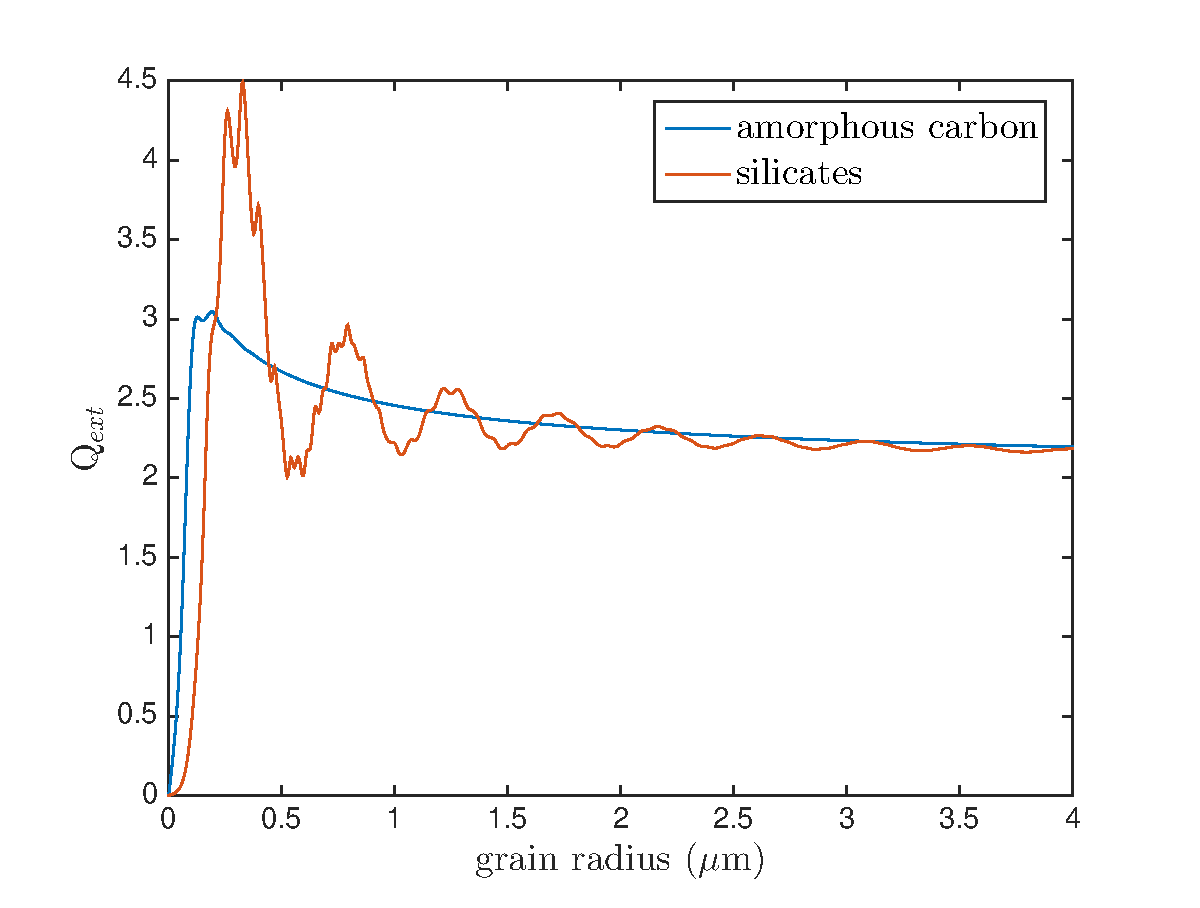
\includegraphics[trim=0 0 0 0,clip=true,scale=0.42]{Qext_grainsize_upto4}
\hspace{3mm}
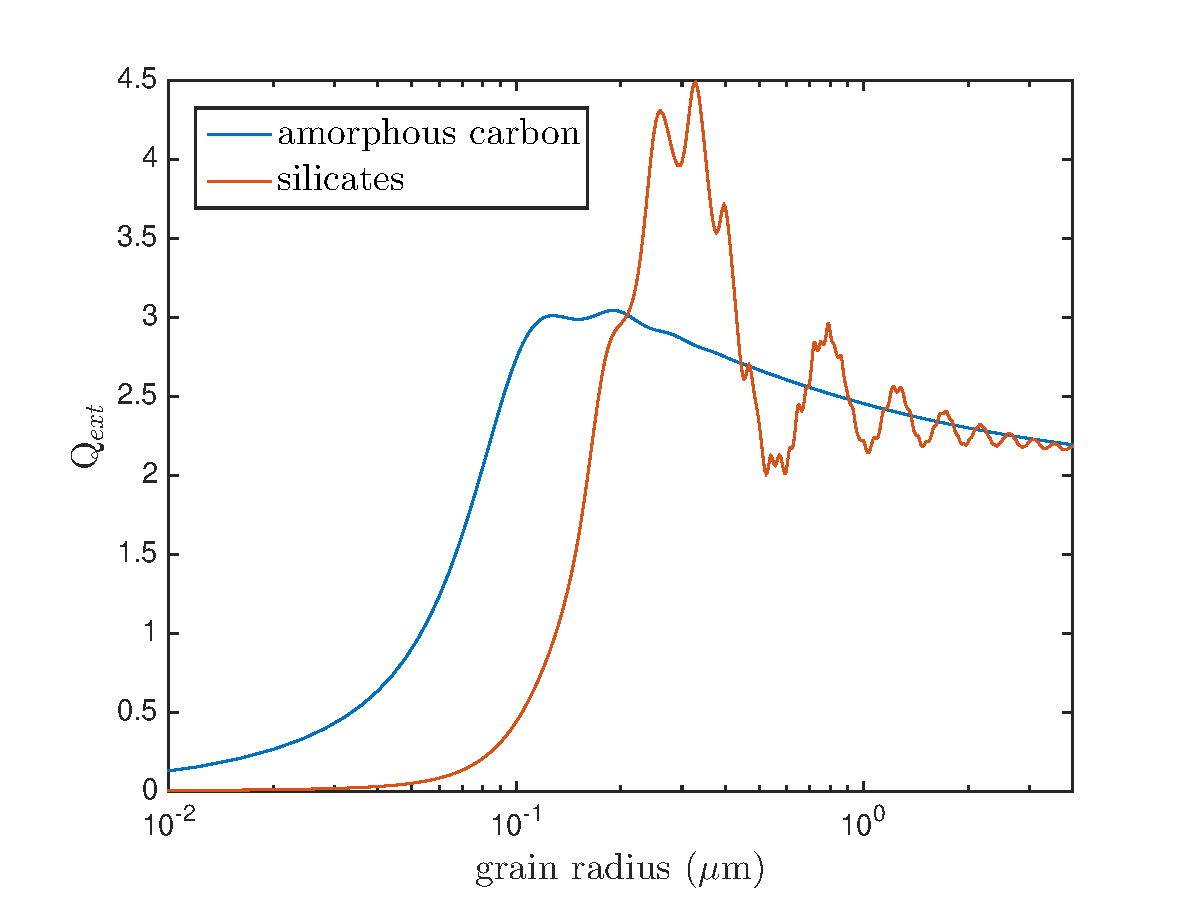
\includegraphics[trim = 0 0 0 0,clip=true,scale=0.42]{Qext_grainsize_upto4_log}
\\
\hspace{0.001mm}
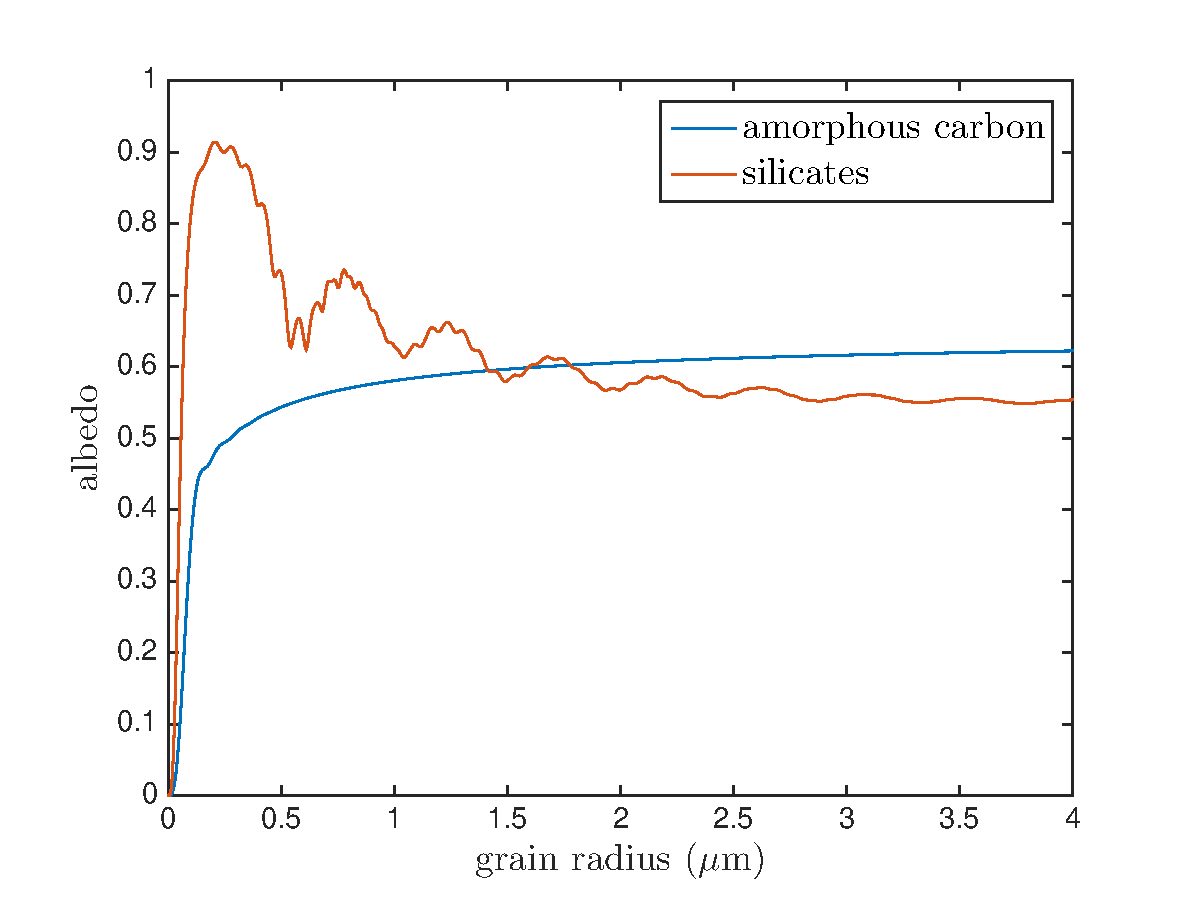
\includegraphics[trim =0 0 0 0,clip=true,scale=0.42]{albedo_grainsize_upto4}
\hspace{3mm}
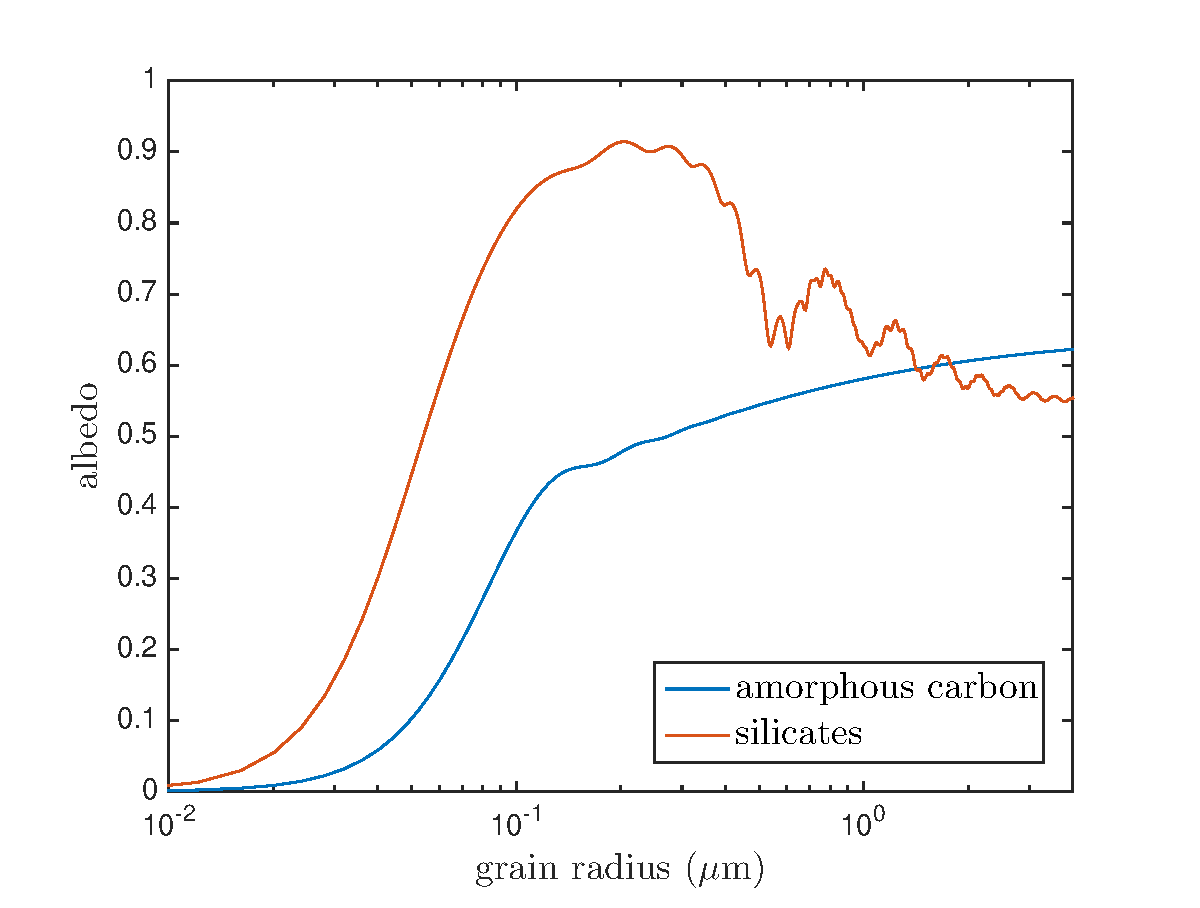
\includegraphics[trim =0 0 0 0,clip=true,scale=0.42]{albedo_grainsize_upto4_log}
\caption{Variation of albedo and extinction efficiency ($Q_{ext}$) with grain size for \citet{Zubko1996} BE amorphous carbon and \citet{Draine1984} silicates using Mie theory at $\lambda = 658 \mu $m. A linear grain size scale is presented on the left and a log scale on the right.}
\label{albedo_grain}

\end{figure*}

The effects of absorption by dust on a line profile for a filled nebula with $R_{in}/R_{out}=0$, as opposed 
to a detached shell, are shown in Figure \ref{fig:Lucy}.  
%The effects of line scatting from moving dust grains are evidenced 
%by the presence of an extended red scattering wing beyond $V_{max}$ as shown in Figure \ref{wt}. 
All profiles have been scaled to unit flux at their peaks.



\subsubsection{The dust optical depth $\tau$ (detached shell case)}
\label{tau}

As expected, greater attenuation of the original line profile is seen on 
the red side (see Figures \ref{wt} and \ref{bt} ).  The profiles are most revealing at lower 
dust optical depths since the effects of the asymmetric absorption can be seen in 
different sections of the profiles and the profiles therefore tend to exhibit more features.
  The region of the profile that is 
most clearly affected by dust absorption is the flat-topped region.  A 
small amount of absorption in this region results in a skewed profile, 
with a fraction of the flat-topped section removed.  The peak becomes 
blue-shifted as a result, but only to the original value of $-V_{min}$, the minimum 
velocity corresponding to $R_{in}$. In addition to the attenuation in this region, 
the red wing of the profile is also somewhat reduced, and the blue wing 
somewhat increased relative to their original symmetric positions.  The 
result is a relatively ``jagged'' looking profile, often with sharp changes 
at $\pm V_{min}$.  The profile is generally asymmetric, although the 
degree of absorption in the flat-topped region may sometimes make it seem 
as though the profile is in fact symmetric and uniformly blue-shifted (see 
Section \ref{asym} for further discussion).  Observationally, these sharp features might become smoothed due to insufficient spectral resolution.

At high dust optical depths or when the ratio of the inner and outer radii is small, the entire profile is shifted to the blue and the 
peak moves beyond $-V_{min}$ further into the blue.  The 
profiles also tend to become more smooth and featureless.  A set of models showing 
the effects of varying optical depths for different density profiles and 
dust albedos are presented in Figures \ref{wt} and \ref{bt}  with $R_{in}/R_{out} = 0.2$.



\subsubsection{The dust albedo $\omega$}
\label{omega}



In the past, there has often been a focus on the effects of absorption by dust 
on the shapes of line profiles and less attention has been paid to the 
potential effects of scattering by dust.  In fact, line profiles 
can be significantly affected by scattering of radiation.  
The greater attenuation of radiation received from the receding portion of 
the ejecta results in an asymmetry of the line profile whereby the 
majority of the observed emission is located bluewards of the peak.  
However, the effects of repeated dust scattering events within the 
ejecta can substantially alter the shape of a line profile and potentially can act to counter the blue-shifted asymmetry.  

Not only does 
repeated scattering of photons increase the number of potential 
opportunities for a given photon to be absorbed but it also results in 
continuous shifting of the frequency of the photon to the red.  The photon 
must do work on the expanding shell of dust in order to escape and thus 
many of the photons are reprocessed beyond the theoretical maximum 
velocity on the red side of the profile.  Even in the case of dust grains 
with a relatively low albedo, a surprisingly persistent wing on the red 
side of the profile is seen, generally beyond the maximum theoretical velocity 
of the emitting region. In the case of strong 
dust scattering and high dust optical depths, this can actively result in a 
shift in the overall asymmetry of the profile, with the majority of the 
emission being emitted redwards of the peak.
The peak however, remains blue-shifted (for example the bottom left panel of Figure \ref{wt}) or central (for example the bottom right panel of Figure \ref{wt}).  
For the line profile to exhibit this feature requires the dust to be a 
nearly perfect scatterer and it is therefore unlikely that profiles of this sort will be
frequently observed.  See Figure \ref{wt} for a fuller illustration of the effects of varying
$\omega$ and $\tau$, and Figure \ref{albedo_grain} for plots of the relationship between albedo and dust grain size.

The combination of relatively low dust optical depths, initially flat-topped 
profiles, greater attenuation on the blue side along with increased flux on the 
red side due to scattering can result in a profile that sometimes  ends up appearing 
almost symmetrical, particularly if 
contaminants, such as narrow lines or blending with other broad lines, are 
present or if the resolution of the data is low.  The potential for apparently 
symmetrical profiles that appear to have been uniformly blue-shifted 
should be noted (see Figures \ref{wt} and \ref{bt}  for examples of this).
%The implications of this result in relation to the use of line profiles as 
%a diagnostic for tracing dust formation in supernova ejecta 
%are discussed further in Section \ref{asym}.

%%%%


%UNCOMMENT FOR THESIS
%This effect is obviously analogous to that of electron scattering which 
%also produces a significant red wing in line profiles \citep{Hillier1991, 
%Auer1972b}. This is an important consideration in both modelling and 
%analysis of spectral line profiles.  DAMOCLES has the capacity to include 
%a basic electron scattering mechanism in order to assess the possibility 
%that any observed red wing might be produced by electron scattering rather 
%than dust scattering.  The red wing observed in line profiles is an 
%excellent diagnostic for determining the overall dust albedo and it is 
%therefore important to establish whether this feature is due to 
%electron or dust scattering or a combination of the two.



%%%






\subsubsection{Density profile $\rho \propto r^{-\beta}$}
\label{beta}

Whilst the density profile of the dust may have some effect on the 
resulting profiles, it is the initial emissivity profile (dependent on the 
gas density profile) that has the greatest effect on the shape of 
the line profile.  In general, the steeper the emissivity distribution, the narrower the line 
profile becomes.  The sides of the line profile may become almost vertical 
for a very steep distribution since the majority of the emission then 
comes from a very narrow velocity range.  
%For a flat-topped profile of 
%fixed width this approximates the square profile produced in the case of 
%an emitting shell with constant velocity.

The dependence of the shape of the line profile on the emissivity distribution
is described analytically in Section \ref{analytics} for the case of very optically thin dust.  However, for even fairly low dust optical depths, the density profile  plays a significant role in determining the shape of the line profile where it is affected by dust absorption.  As previously discussed, at relatively small optical depths for reasonable $R_{in}/R_{out}$, 
a section of the flat-topped region is removed resulting in a peak at 
$-V_{min}$.  The shape of the profile in this region is significantly 
affected by the density profile.  Shallow density profiles (low $\beta$) produce a virtually 
linear variation in flux between $-V_{min}$ and $+V_{min}$ (for example the profiles in the left column of Figure \ref{bt}).  For a fixed dust
optical depth, the steeper the distribution becomes, the more concave the 
profile becomes between $-V_{min}$ and $+V_{min}$, ultimately resulting in 
a clear shoulder to the profile at $+V_{min}$  (for example the profiles in the right column of Figure \ref{bt}).  For extremely steep density
distributions this can result in a double peaked profile with 
a trough to the red of $V=0$.  A illustration of the effects on the line profiles of varying $\beta$ and $\tau$  is shown in Figure \ref{bt}.  As previously noted, these features may not be apparent in observed line profiles with poor spectral resolution due to blending.

\subsection{Inferring properties of the dust from the models}




%\begin{figure}
%\begin{center}
%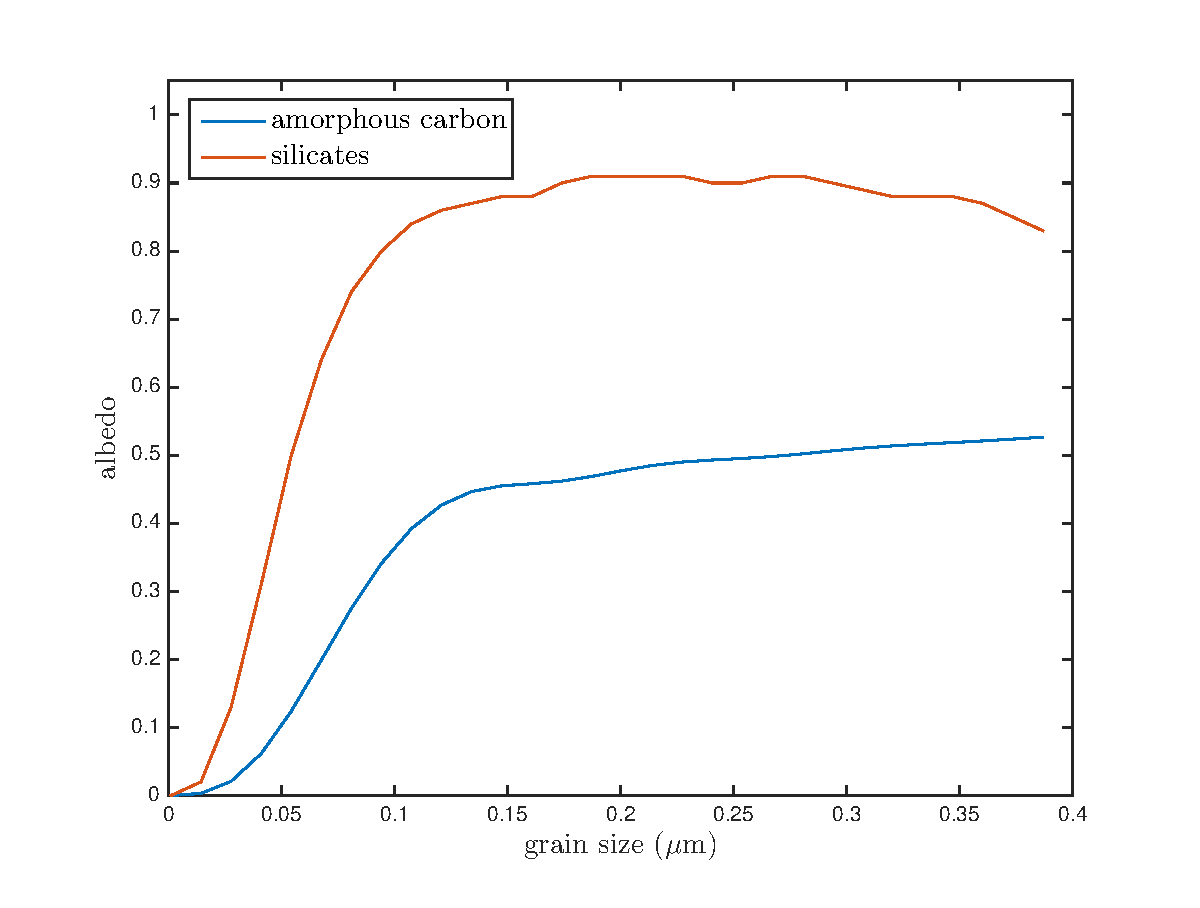
\includegraphics[trim =37 10 45 15,clip=true,scale=0.51]{grainsize_albedo}
%\caption{Variation of albedo with grain size for amorpous carbon sample 
%using a Mie approximation at $\lambda = 658 \mu $m. Optical constants 
%from \citet{Zubko1996}.}
%\label{albedo_grain}
%\end{center}
%\end{figure}

The presence of an extended red wing at large positive velocities in 
combination with increased extinction on the red side at smaller positive 
velocities can allow the values of $\tau$ and $\omega$ to be well 
constrained.  Where this occurs it is possible to translate these values into a 
dust mass and grain size for a given species or combination of 
species using grain optical properties and Mie theory (see Figure 
\ref{albedo_grain}).  
%In fact, it is the dust mass and average grain size 
%that is varied within the code for a specified species or combination of 
%species.  


For amorphous carbon, albedo generally increases with grain size.  The presence and extent of any scattering wing on the red side of the observed profile can therefore help to place limits on the grain radius.  However, the greater the grain radius used the smaller the available cross-section for interaction.  Larger masses of dust 
are therefore required to fit the same degree of absorption if a larger 
grain size is used.  This is in contrast to SED radiative transfer 
modelling where larger grain sizes generally result in less dust being 
required to fit the IR portion of the SED (W15).  These two techniques in 
tandem may therefore provide limits on grain sizes for different 
species or combinations thereof.

It is known that the use of different 
optical properties may substantially alter dust masses derived using SED fitting for a given species of specific grain size (e.g. \citet{Owen2015}).  However, the use of different sets of optical properties in our models seems to have only a minor effect on our results.

\begin{figure*}
\includegraphics[clip=true,scale=0.34]{a0_001_opt_thin_HaHbPad}
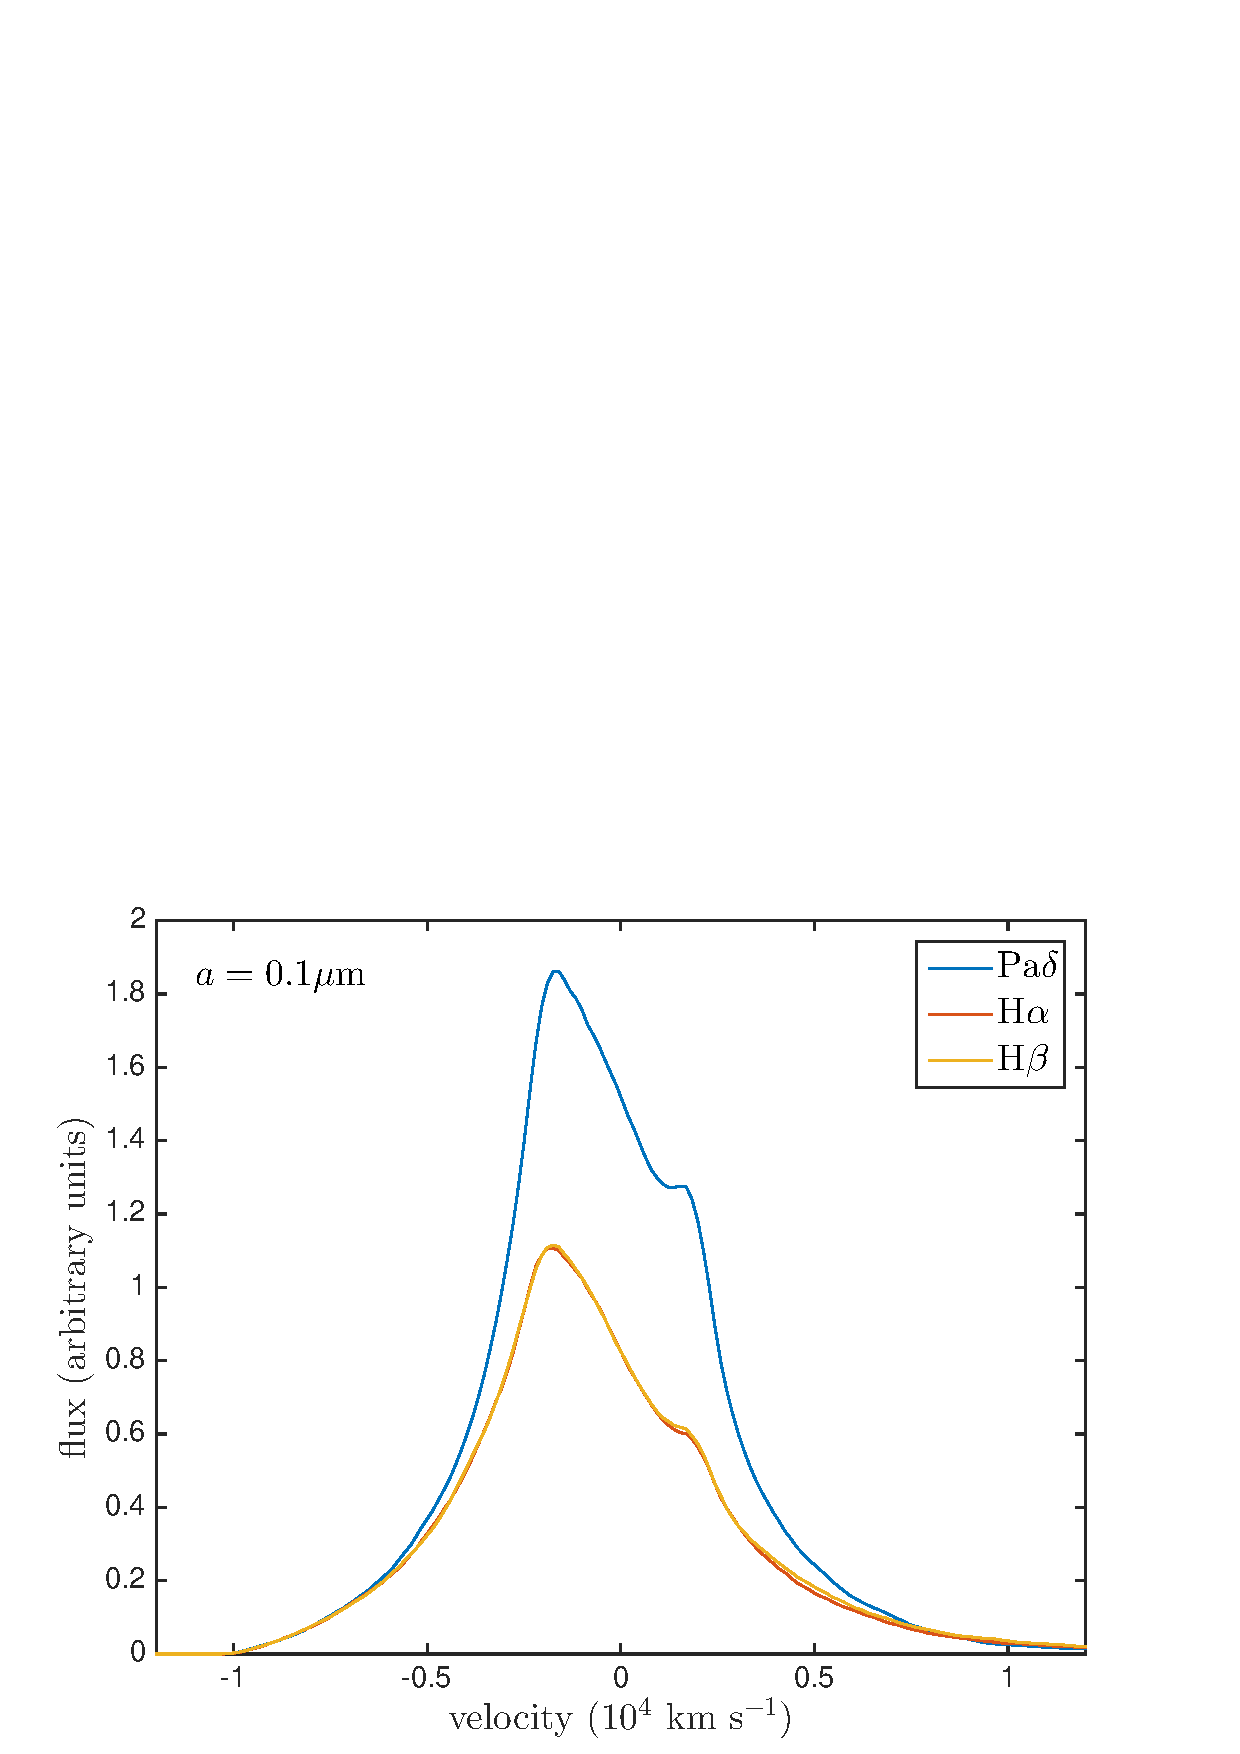
\includegraphics[trim=18 0 0 0,clip=true,scale=0.34]{a0_1_opt_thin_HaHbPad}
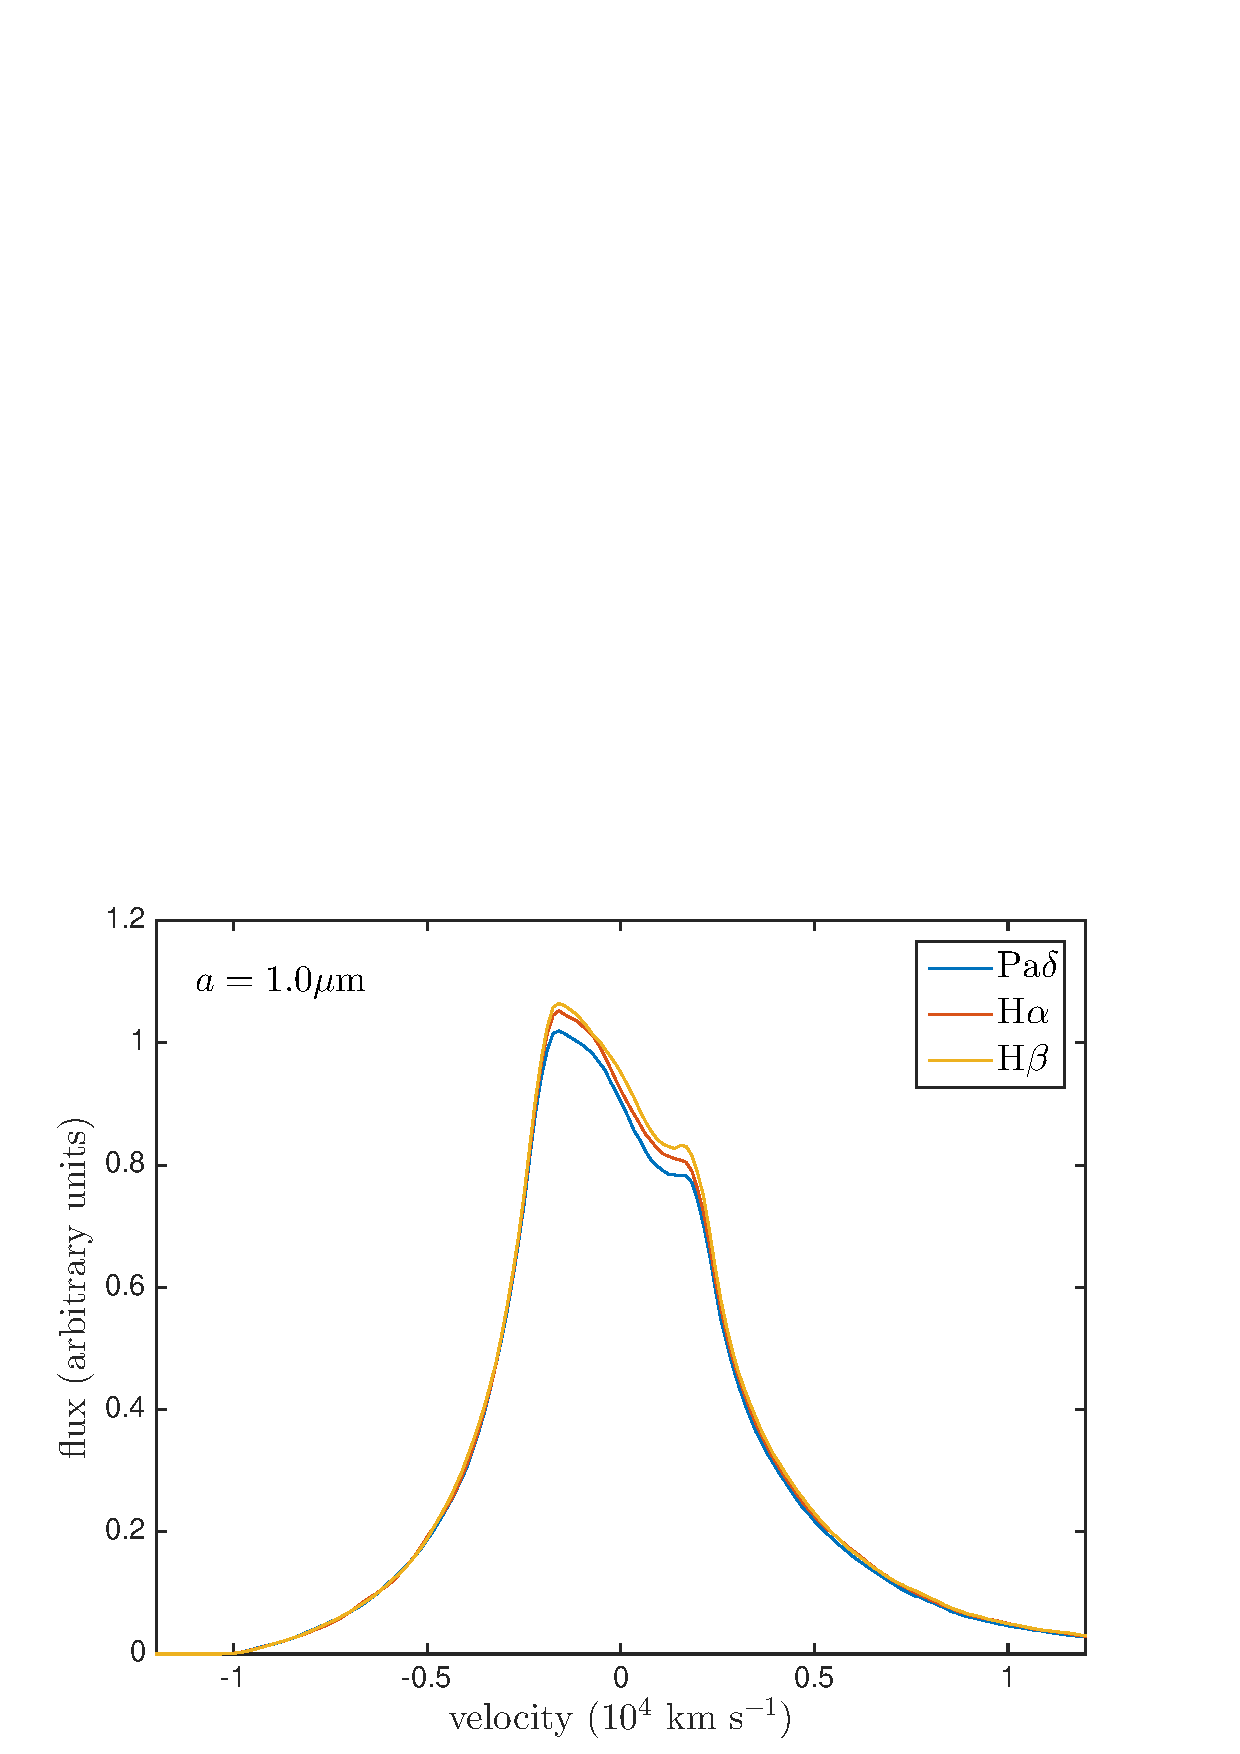
\includegraphics[trim=18 0 0 0,clip=true,scale=0.34]{a1_opt_thin_HaHbPad}

\vspace{1mm}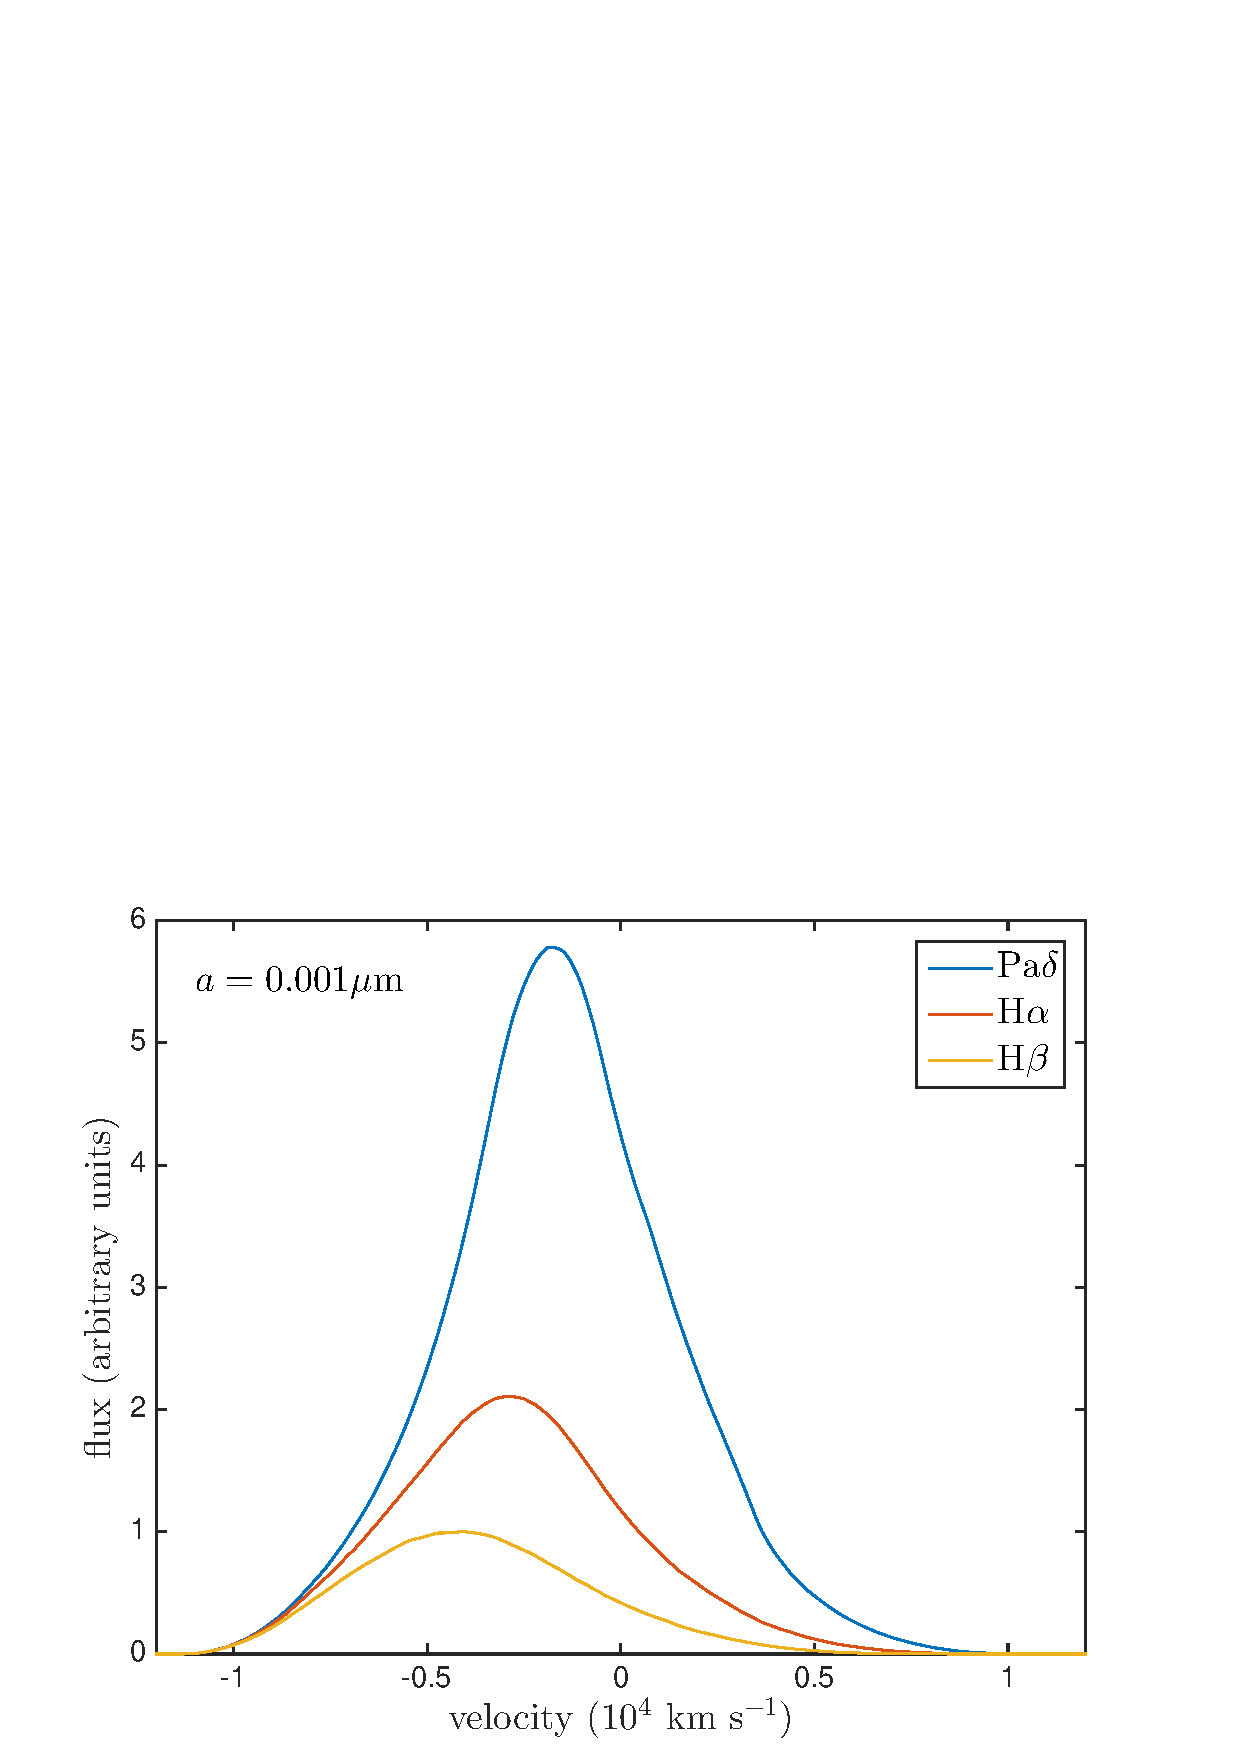
\includegraphics[trim=-18 0 0 0,clip=true,scale=0.34]{a0_001_opt_thick_HaHbPad}
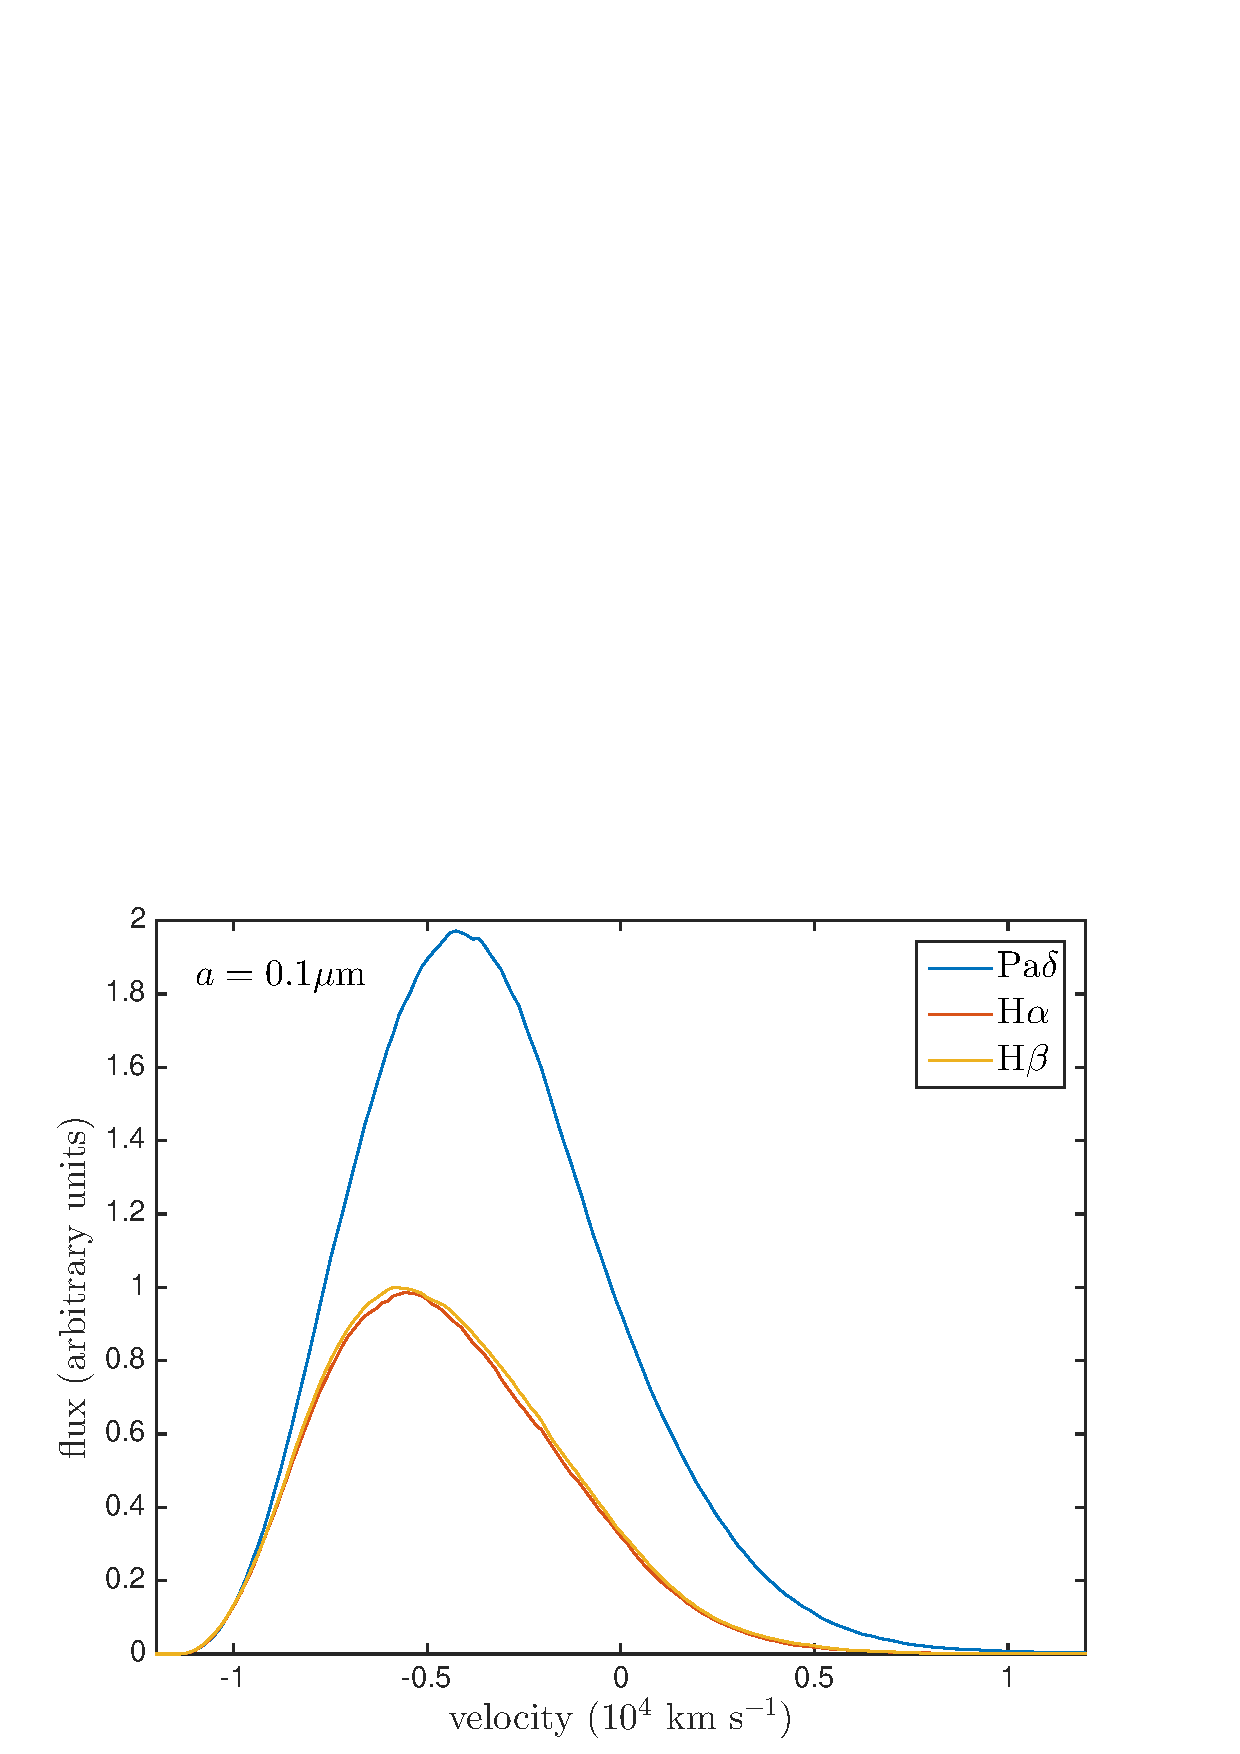
\includegraphics[trim=18 0 0 0,clip=true,scale=0.34]{a0_1_opt_thick_HaHbPad}
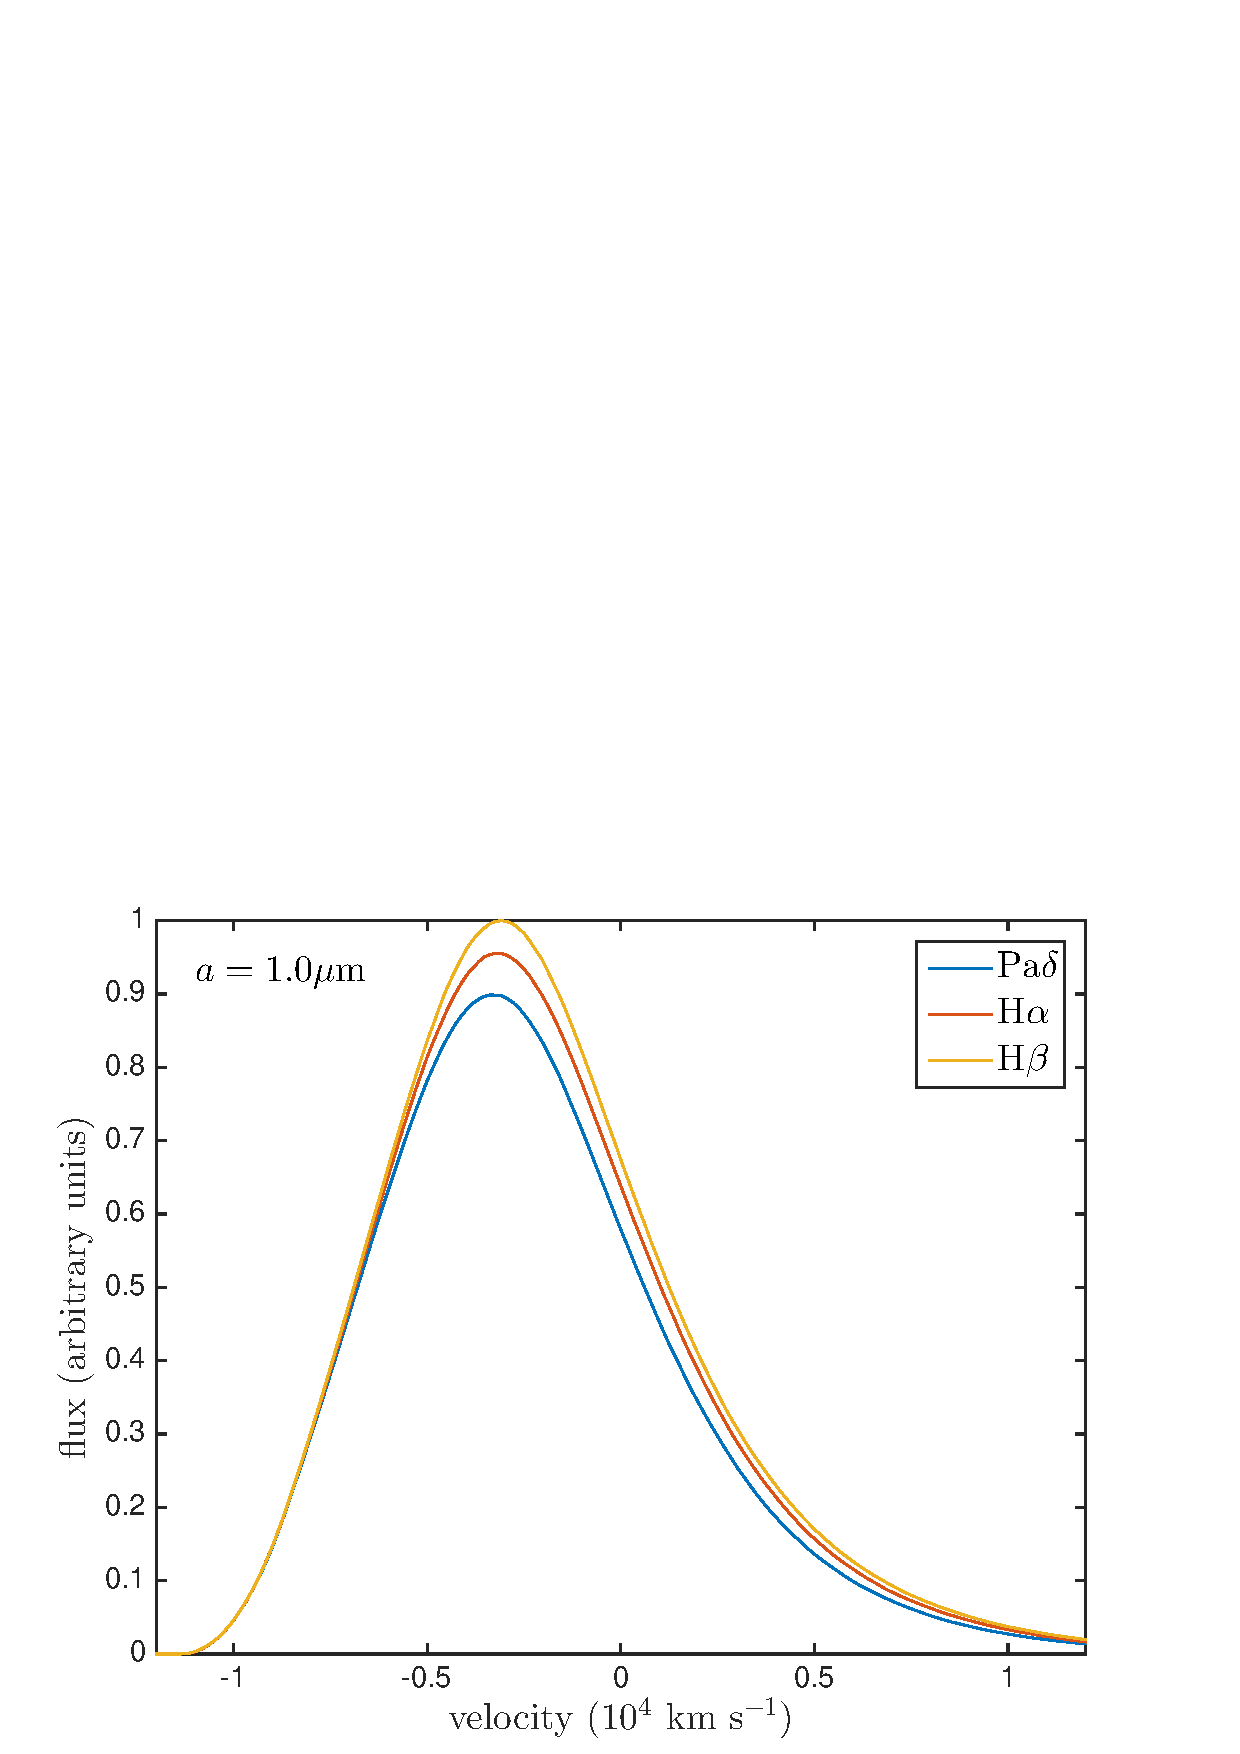
\includegraphics[trim=18 0 0 0,clip=true,scale=0.34]{a1_opt_thick_HaHbPad}
\caption{Model line profiles for H$\alpha$ (6563\AA\ in \textit{red}), H$\beta$ (4861\AA\ in \textit{yellow}) and Pa$\delta$ (10049\AA\ in \textit{blue}) for optically thin \textit{(upper)} and  optically thick \textit{(lower)} cases respectively.  All models adopted density profile $\rho(r) \propto r^{-4}$ (i.e. $\beta = 2$), velocity profiles $v(r) \propto r$ and radii ratio $R_{in}/R_{out}=0.2$.  The grain radii used were $a=0.001~\mu$m \textit{(left)}, $a=0.1~\mu$m \textit{(middle)} and $a=1.0~\mu$m \textit{(right)}. All the above models used amorphous carbon.}
\label{wav_dep}
\end{figure*}

\begin{figure*}
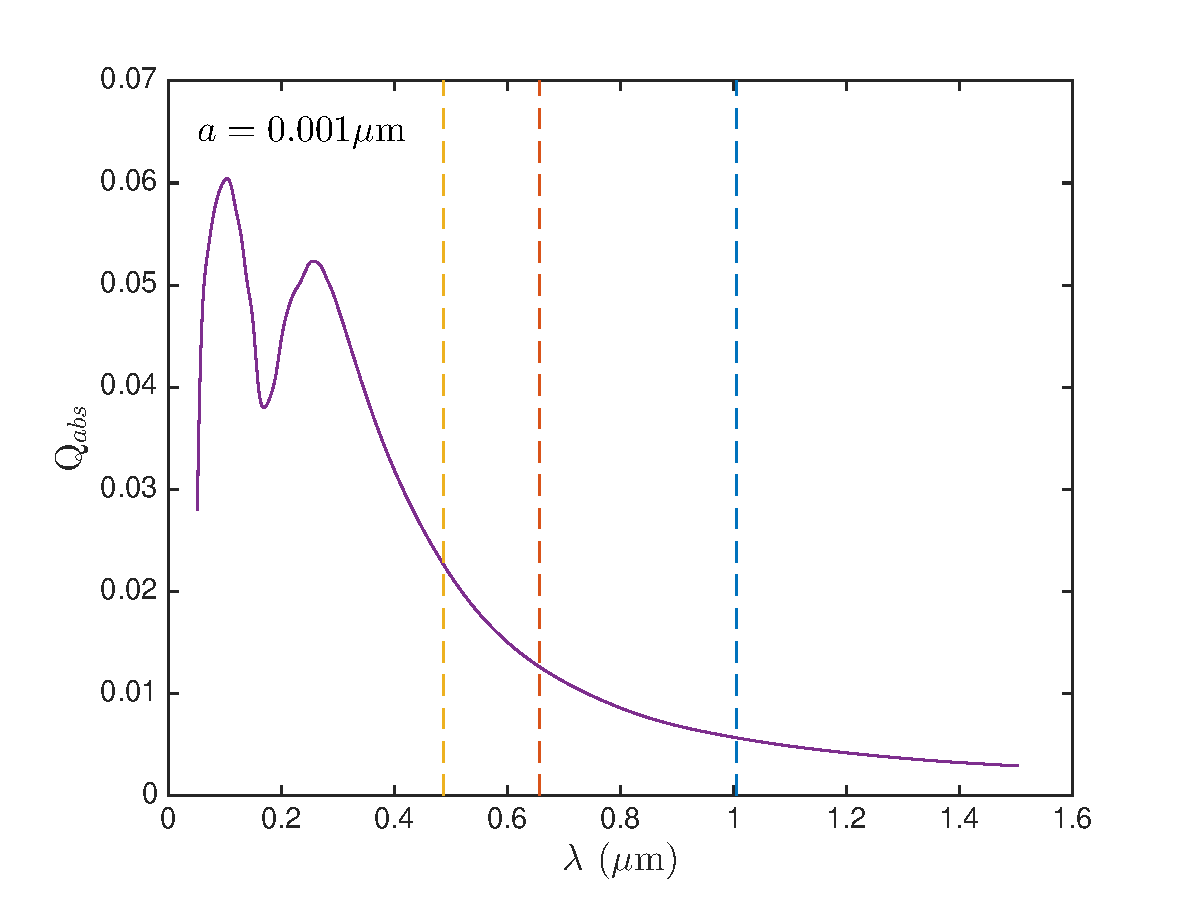
\includegraphics[trim =15 0 45 0,clip=true,scale=0.33]{Qabs_a0_001} \hspace{0.5mm}
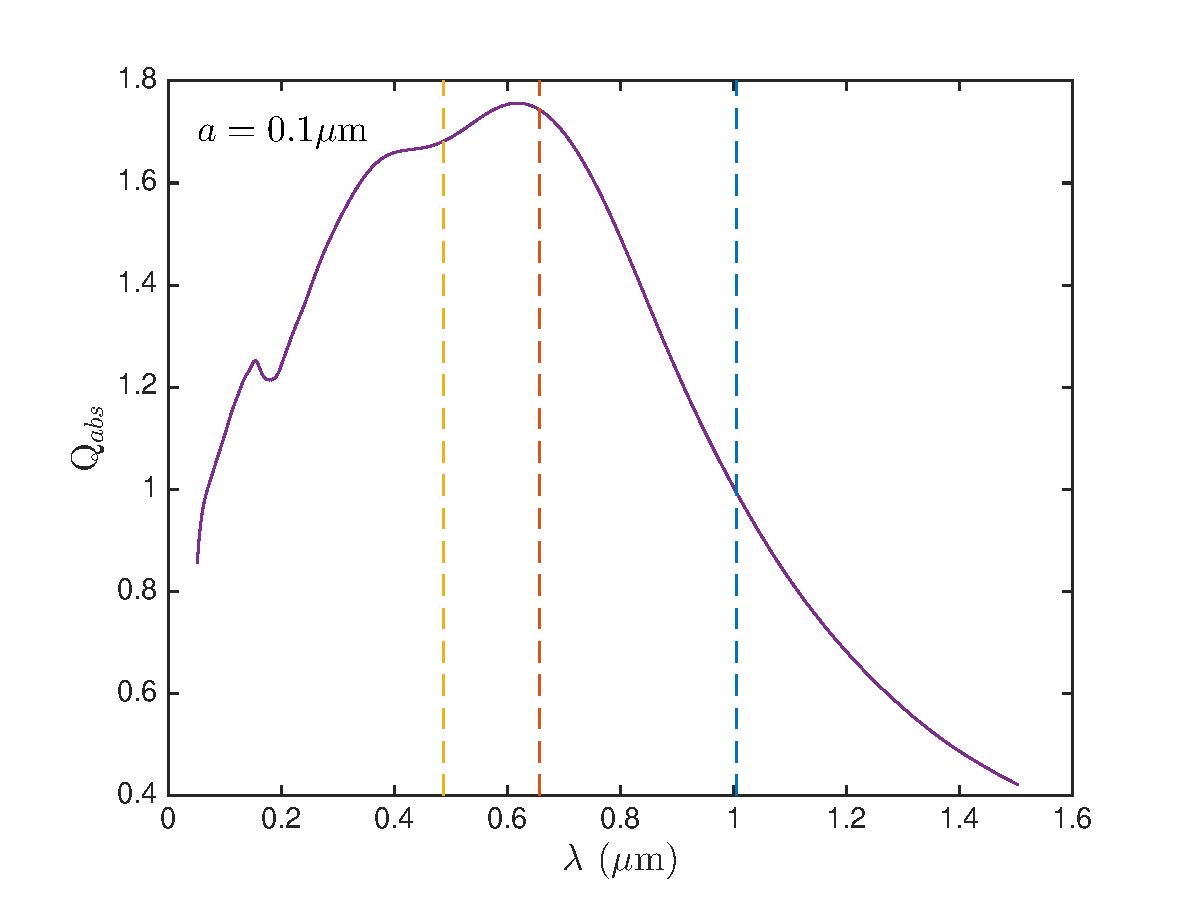
\includegraphics[trim =45 0 45 0,clip=true,scale=0.33]{Qabs_a0_1} \hspace{0.5mm}
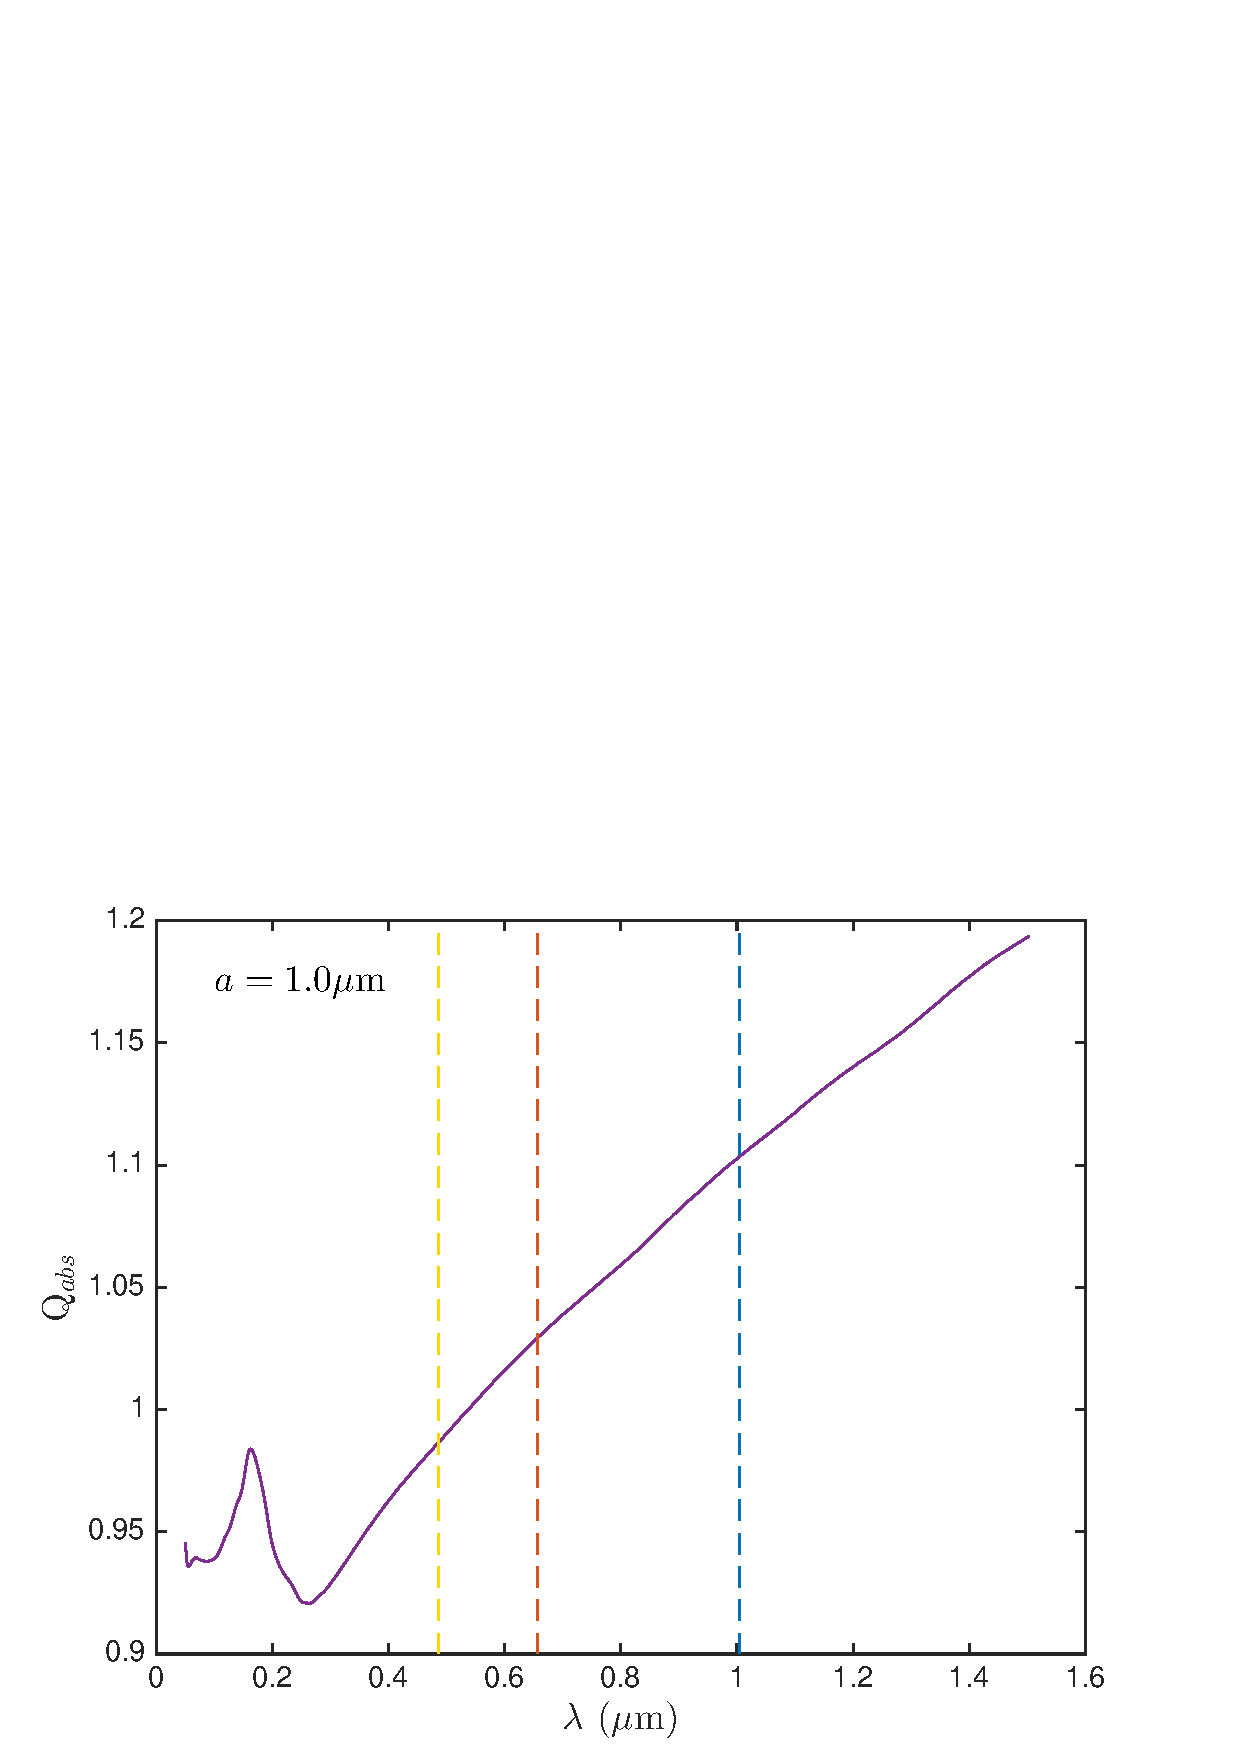
\includegraphics[trim =20 0 5 0,clip=true,scale=0.33]{Qabs_a1_0}
\caption{The variation of amorphous carbon dust absorption efficiency with grain size. The grain radii plotted are $a=0.001~\mu$m \textit{(left)}, $a=0.1~\mu$m (middle) and $a=1.0~\mu$m \textit{(right)}.  The vertical lines mark the wavelengths of H$\alpha$ (6563\AA\ in red), H$\beta$ (4861\AA\ in yellow) and Pa$\delta$ (10049\AA\ in blue).}
\label{wav_dep2}
\end{figure*}






\subsection{The wavelength dependence of dust absorption}
%{Observable signatures of dust in line profiles}
\label{asym}

The greater the dust optical depth, the more attenuation of the line 
there is.  As expected, the red side of the profile suffers a greater 
degree of absorption than the blue side.  The resulting asymmetry is 
somewhat more complex than perhaps previously thought.  Dust has 
repeatedly been cited as the agent responsible for the apparent 
blue-shifting of supernova line profiles in the manner of the profiles 
presented in Figure \ref{fig:Lucy}; that is, relatively high optical 
depths result in an overall shift of the entire profile towards the blue.
 The relationship between the blueshifting of the peaks 
of profiles and their wavelength has been discussed by several authors in 
relation to dust formation \citep{Smith2012, Fransson2014, Gall2014}.  
  
In practice a relatively  large dust optical depth is 
required to actively shift the peak of the profile bluewards of its natural 
$-V_{min}$ position (corresponding to the velocity at the inner radius of the shell) unless this value is very small in comparison to $V_{max}$ i.e. the profile originally had a very narrow flat top.  
In many cases it seems likely that the dust
may not be optically thick and the blue-shifting of the peak of the profile just
 a result of attenuation in the flat-topped section (close to 
$R_{in}$).  The peak would then tend to be located at $-V_{min}$.

Since dust absorption is wavelength dependent for $2\pi a < \lambda$, one might expect the 
position of the peak line flux to be dependent on the wavelength of the line being 
considered.  We note here that whilst variations of the peak velocity of a line as a function of line wavelength 
may occur in cases of high dust optical depths or small $R_{in}/R_{out}$, this may 
not be the case for many supernova lines emitted from ejecta with low dust optical depths.  
The wavelength-dependence of dust absorption instead 
can result in differing degrees of extinction in the flat-topped region of 
each profile but still leave the peak at its blue-shifted position of 
$-V_{min}$.  If this is the case then there would be no 
reason to expect a variation in the position of the peaks of profiles to be 
correlated with the wavelength dependence of dust absorption.  Instead one would 
expect it potentially to trace the location of different ions within the ejecta, possibly with different $V_{min}$ values observed for  
different species.  

For lines from the same ion, for example the Balmer and Paschen lines of HI,
we might expect to see peaks at the same position but differing degrees of absorption.
At high spectral resolutions, it might be possible to detect differences in the shapes of the line 
profiles, particularly between $-V_{min}$ and $+V_{min}$ where the steepness of the 
incline traces the degree of dust absorption.  This can be seen in Figure \ref{wav_dep} 
where we illustrate the effects of the wavelength dependence of dust absorption for 
three lines, H$\alpha$ (6563\AA), H$\beta$ (4861\AA) and Pa$\delta$ (10049\AA).  
All lines were modelled using three different grain sizes and for both optically thin and 
thick dust cases.  We also show the variation of the absorption efficiency with 
wavelength for three different amorphous carbon grain sizes in Figure \ref{wav_dep2}.

%UNCOMMENT FOR THESIS
%The attenuation of the flat-topped region is also often such that it can 
%be hard to discern a difference in slope in the attenuated 
%section between $-V_{min}$ and $+V_{min}$ and the slope of the wing for 
%$V>+V_{min}$, particularly in circumstances where data are of poor 
%resolution or have a poor signal-to-noise ratio.  Even in the case of 
%excellent data, it may be easy to overlook these particular features or to 
%dismiss them as natural fluctuations in the geometry of the ejecta rather than 
%that they may be a product of dust absorption effects.



\section{Results for SN~1987A}
\label{results}

\begin{figure}
\begin{center}
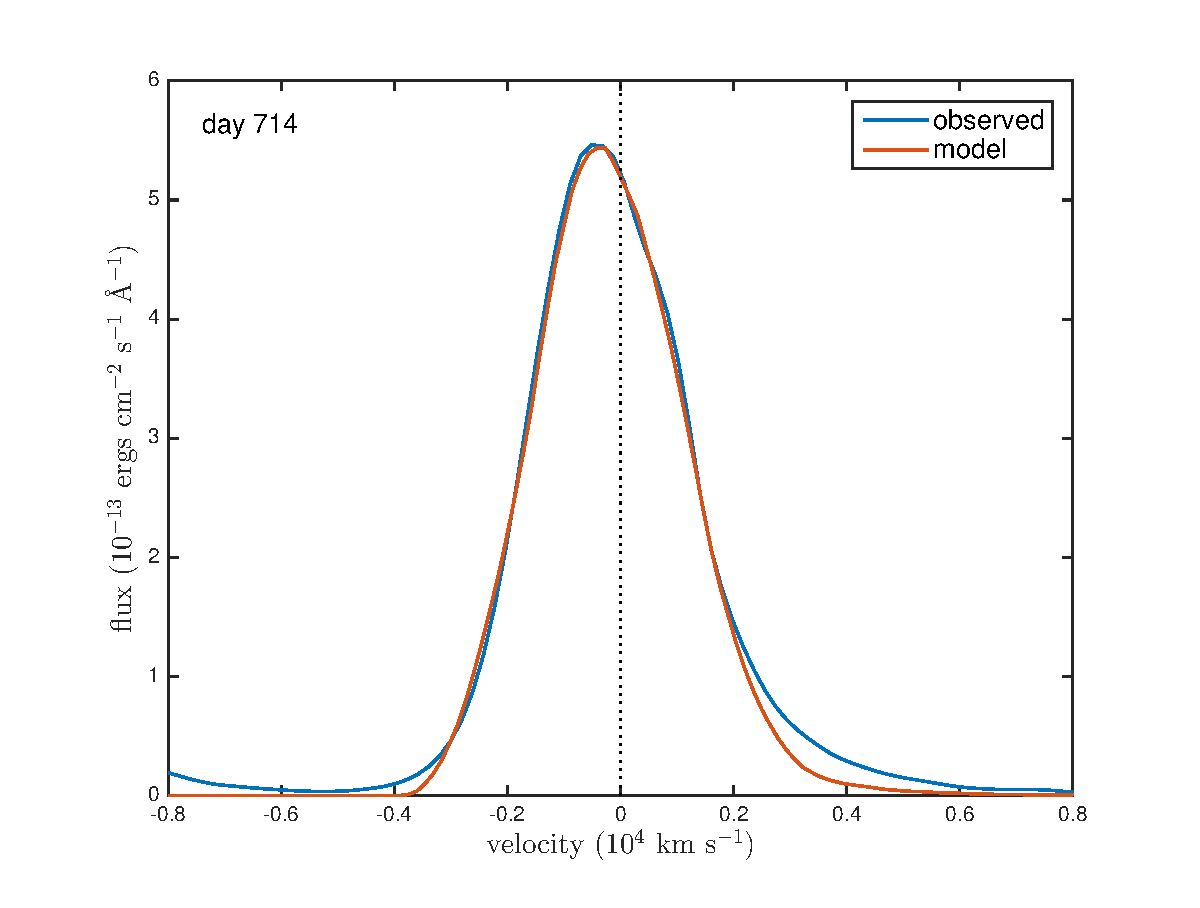
\includegraphics[trim =33 10 45 15,clip=true,scale=0.51]{smooth/d714Ha_smooth_amC_MRN}
\caption{MRN smooth dust fit to the day 714 H$\alpha$ line of SN~1987A illustrating the 
underestimation of the red scattering wing for small grain sizes.  Model 
parameters are the same as the smooth dust fit for day 714 (Table \ref{smooth1}) except for the 
grain size distribution and dust mass:  $M_{dust}=8.0 \times 10^{-6} 
M_{\odot}$, $a_{min}=0.005 \mu$m, $a_{max}=0.25 \mu$m and $n(a) \propto 
a^{-3.5}$.}
\label{MRN}
\end{center}
\end{figure}

\begin{figure*}
\begin{center}
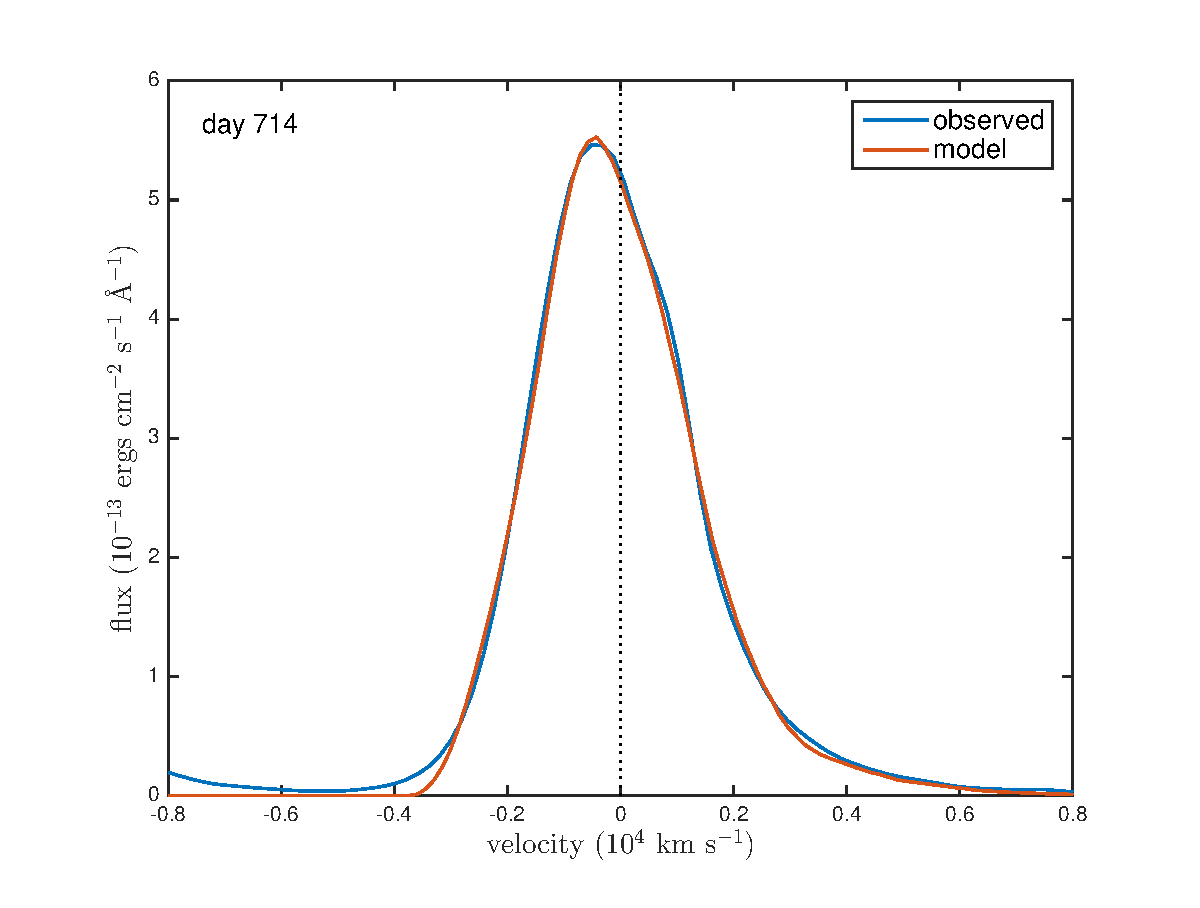
\includegraphics[trim =33 10 45 15,clip=true,scale=0.47]{smooth/best_fit/d714Ha}
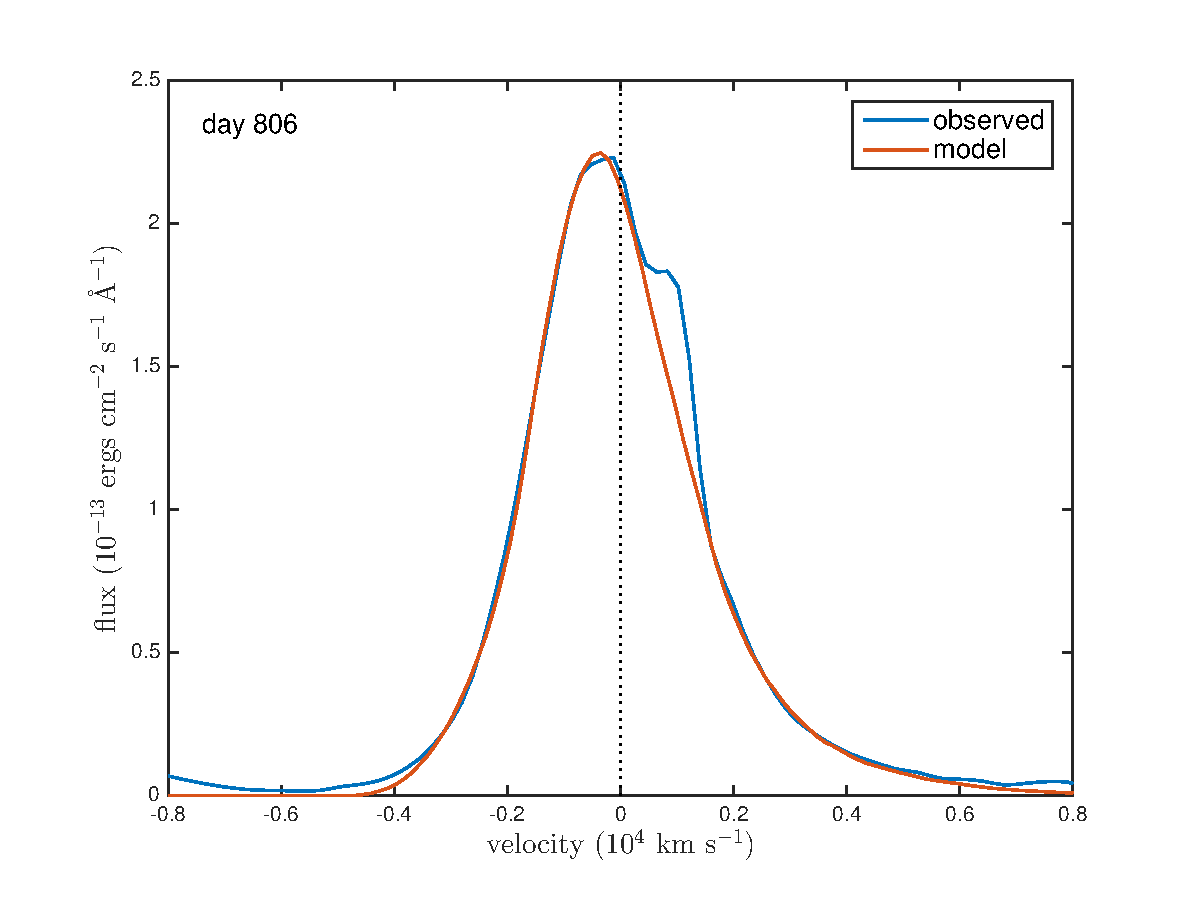
\includegraphics[trim =33 10 45 15,clip=true,scale=0.47]{smooth/best_fit/d806Ha_new}
\caption{Best smooth dust fit to the SN~1987A H$\alpha$ line at day 714 \textit{\textit{(left)}} and day 806 \textit{\textit{(right)}} for the parameters detailed in Table \ref{smooth1} with amorphous carbon grains of radius $a=0.35 \mu$m.}
\label{Ha_smooth}
\end{center}
\end{figure*}
\begin{figure*}
\begin{center}

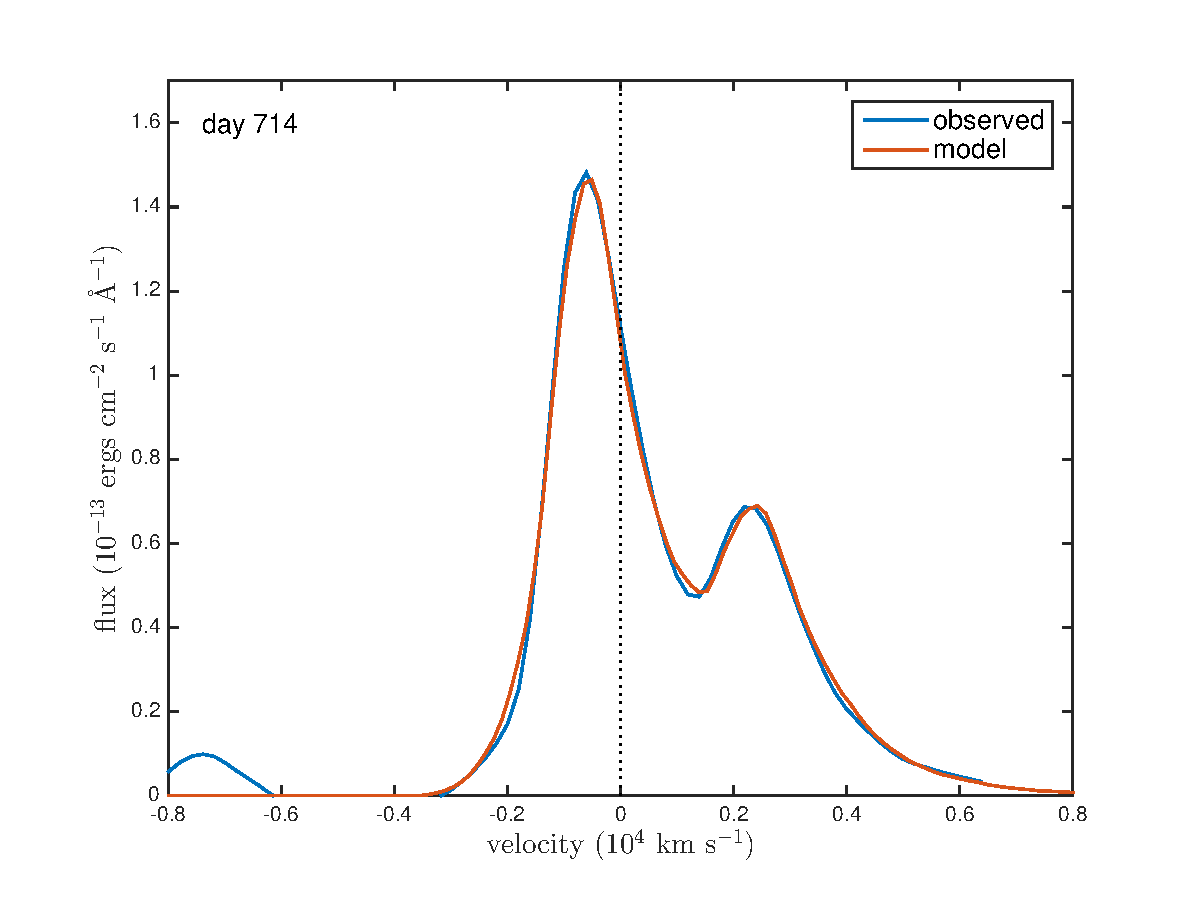
\includegraphics[trim =33 10 45 15,clip=true,scale=0.47]{smooth/best_fit/d714OI_new}
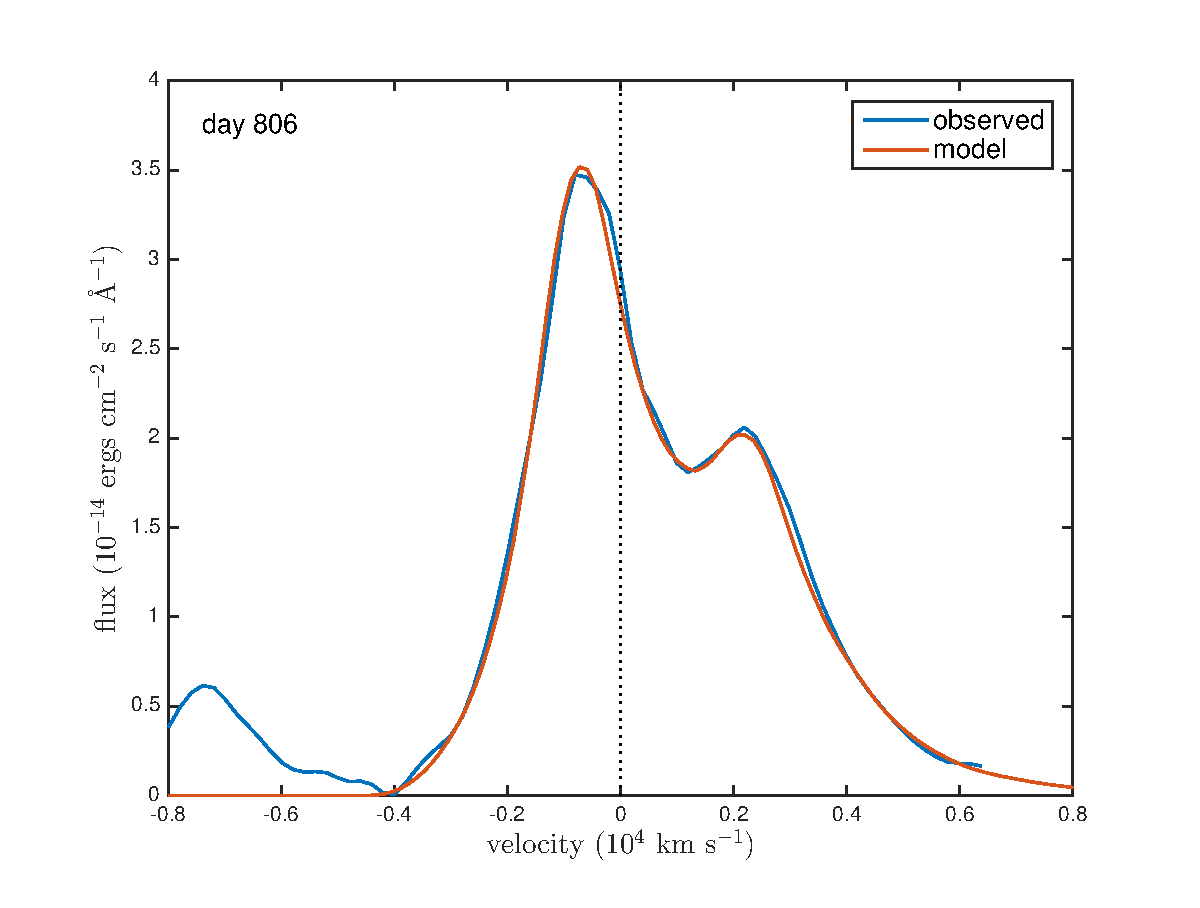
\includegraphics[trim =33 10 45 15,clip=true,scale=0.47]{smooth/best_fit/d806OI_new}
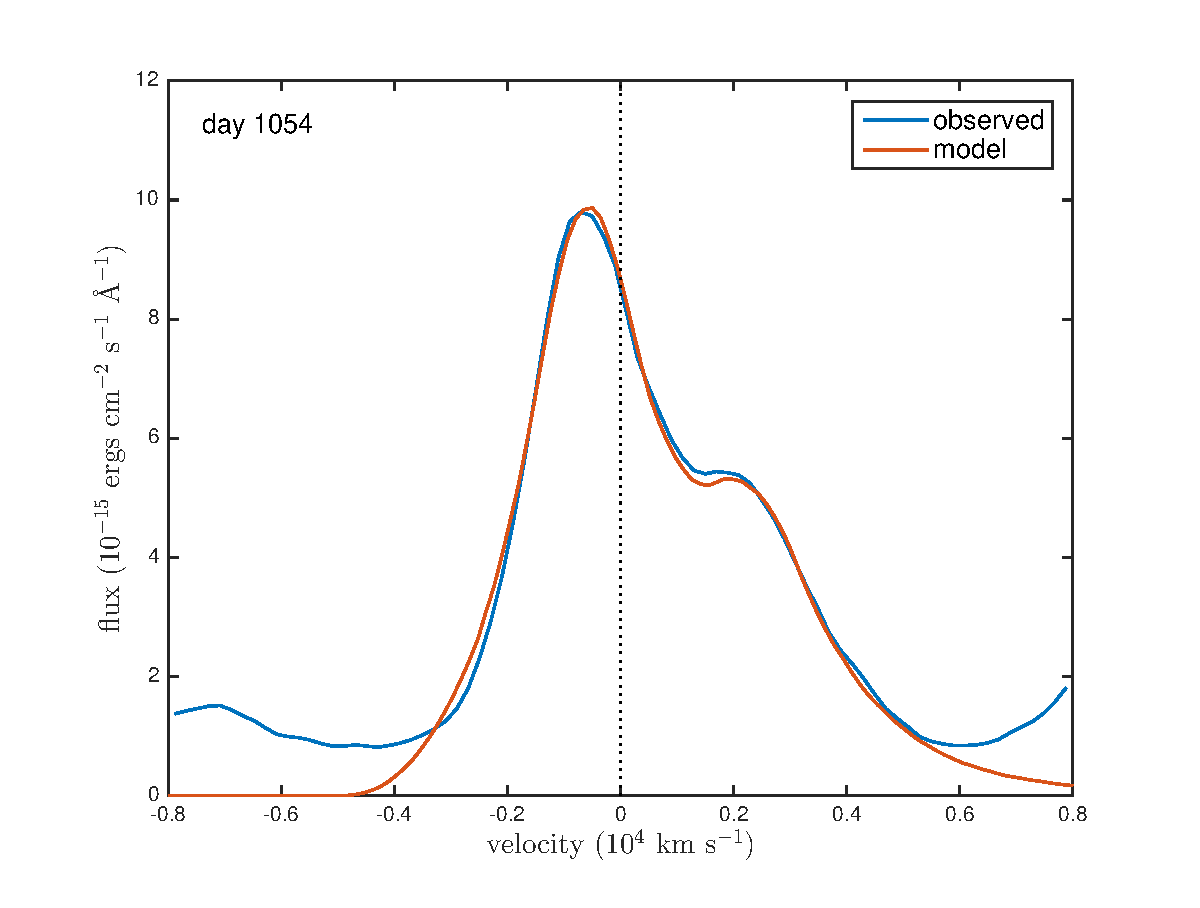
\includegraphics[trim =33 10 45 15,clip=true,scale=0.47]{smooth/best_fit/d1054OI}
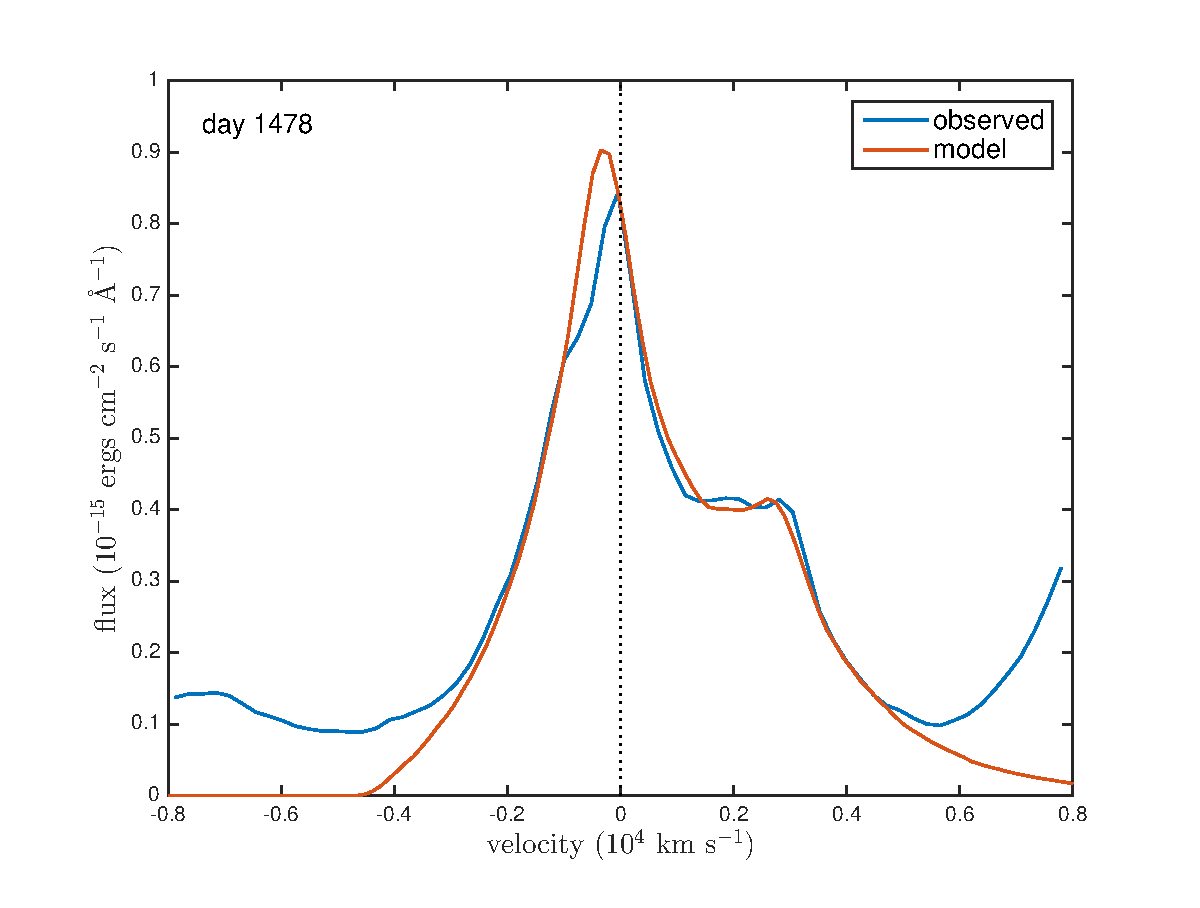
\includegraphics[trim =33 10 45 15,clip=true,scale=0.47]{smooth/best_fit/d1478OI}
\caption{Best smooth dust fit to the SN~1987A [O~{\sc i}]~$\lambda$6300,6363~\AA\ doublet at day 714 \textit{(upper left)}, day 806 \textit{(upper right)}, day 1054 \textit{(lower left)} and day 1478 \textit{(lower right)} for the parameters detailed in Table \ref{smooth1} with amorphous carbon grains of radius $a=0.35 \mu$m..}
\label{OI_smooth}
\end{center}
\end{figure*}


We have  modelled the H$\alpha$ line of SN~1987A at days 714, 806, 1862, 2211, 2875, 3500 and 3604, and the 
[O~{\sc i}]~$\lambda$6300,6363~\AA\ doublet at days 714, 806, 1054 and 1478.  After day 3604 the H$\alpha$ profile begins to become dominated by emission from the reverse shock 
and the structure of the emitting region may no longer be approximated by 
a single shell model as we do here \citep{Fransson2013}.  The [O~{\sc i}]~$\lambda$6300,6363~\AA\ doublet becomes too weak to model after day 1478  (see Figure \ref{Ha_evol_early}).  We continue to adopt a velocity profile $V(r) = 
\frac{V_{max}}{R_{max}}r$ and treat the variable parameters listed at the start of 
Section \ref{ps}.  Whilst the albedo and optical depth are not varied 
directly, they are altered by adjusting the dust mass, $M_{dust}$, and the 
grain size, $a$, which together determine the albedo and optical 
depth via  Mie theory and the optical properties of the 
dust.

\begin{table}
\caption{Observed luminosities of the H$\alpha$ line and estimated electron scattering optical depths from $R_{in}$ to $R_{out}$ for the radii detailed in Tables \ref{smooth1} to \ref{clumped1} based on an assumed gas temperature of 10,000K.}
\begin{center}
\begin{tabular}{@{}ccccc@{}}
\hline
day & observed $L_{H\alpha}$ & undepleted $L_{H\alpha}$ & absorbed  & $\tau_e$ \\
& (10$^{37}$ erg s$^{-1}$) & (10$^{37}$ erg s$^{-1}$) & fraction & ($10^{-2}$) \\
\hline
714 & 1.36 & 2.24 &0.39& 1.44  \\
806 & 0.57 & 1.01 &0.43& 0.840 \\
1862 & 0.0063 & 0.013 &0.50& 0.159  \\
2211 & 0.0041 &0.0085 &0.51& 0.0378  \\
2875 & 0.0019 & 0.0054& 0.65 &0.0219  \\
3500 & 0.00079 & 0.0025 & 0.69&0.0125  \\
3604 & 0.00098 & 0.0032 &0.69&0.0149  \\

\hline
\end{tabular}
\end{center}
\label{tau_e}
\end{table}%



In all models, the ejecta occupies a shell with inner radius $R_{in}$ and 
outer radius $R_{out}$.  Packets are emitted according to a smooth density 
profile assuming recombination or collisional excitation such that $i(r) \propto \rho(r)^2 \propto 
r^{-2\beta}$.  Initially the dust is considered to have a smooth density 
distribution and is assumed to be coupled to the gas so as to follow the same 
radial profile.  A clumped distribution of dust is considered later (see 
Section \ref{clumped_models}).  

We estimate the electron scattering optical depths at a temperature of 10,000K between $R_{in}$ and $R_{out}$ based on the observed fluxes of the H$\alpha$ line.  A temperature of 10,000K is likely too high at the epochs considered but we adopt it in order to be sure not to underestimate electron scattering optical depths.  The values we calculate and the observed H$\alpha$ luminosities are listed in Table \ref{tau_e}.  The  electron scattering optical depths are negligibly small and we therefore do not include electron scattering in 
these models.


\begin{figure*}
\begin{center}
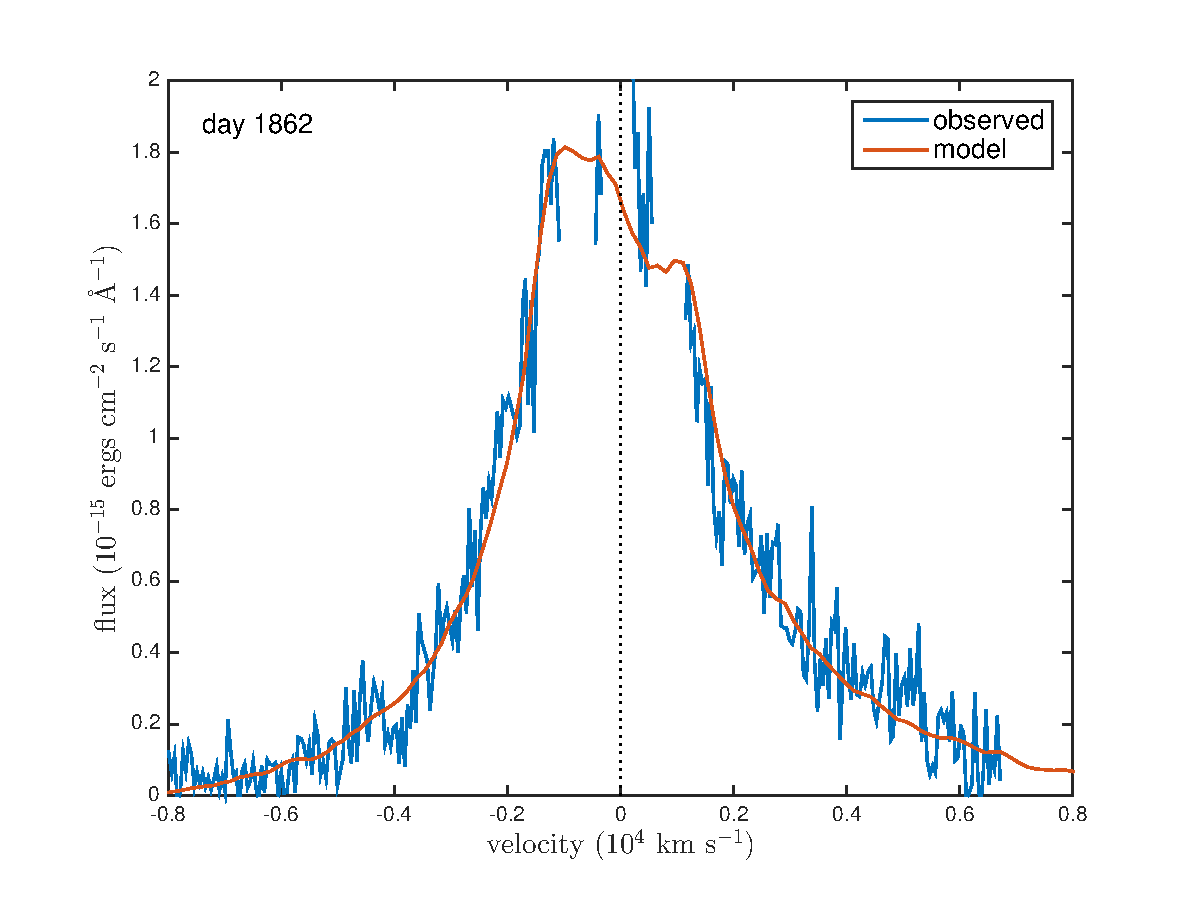
\includegraphics[trim =33 10 45 15,clip=true,scale=0.35]{smooth/best_fit/d1862Ha}
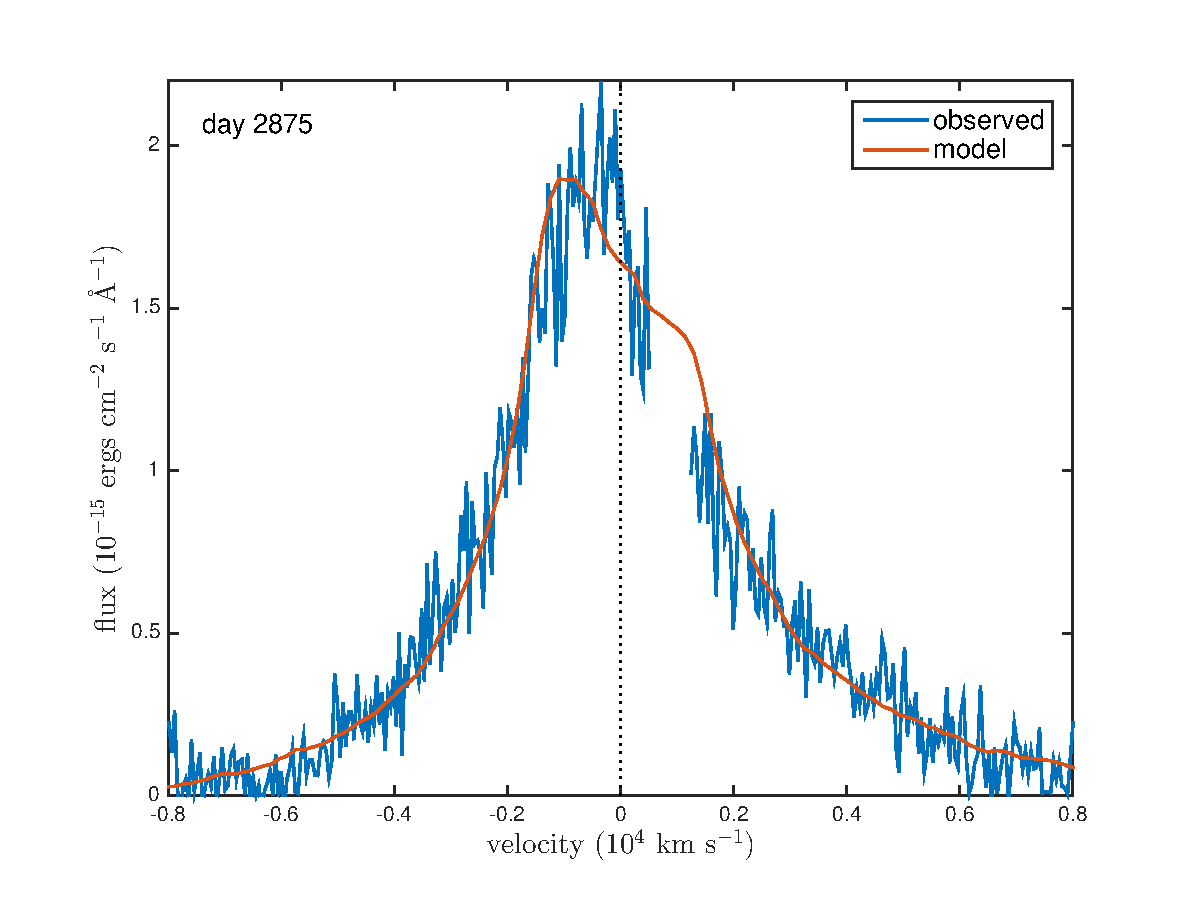
\includegraphics[trim =55 10 45 15,clip=true,scale=0.35]{smooth/best_fit/d2875Ha}
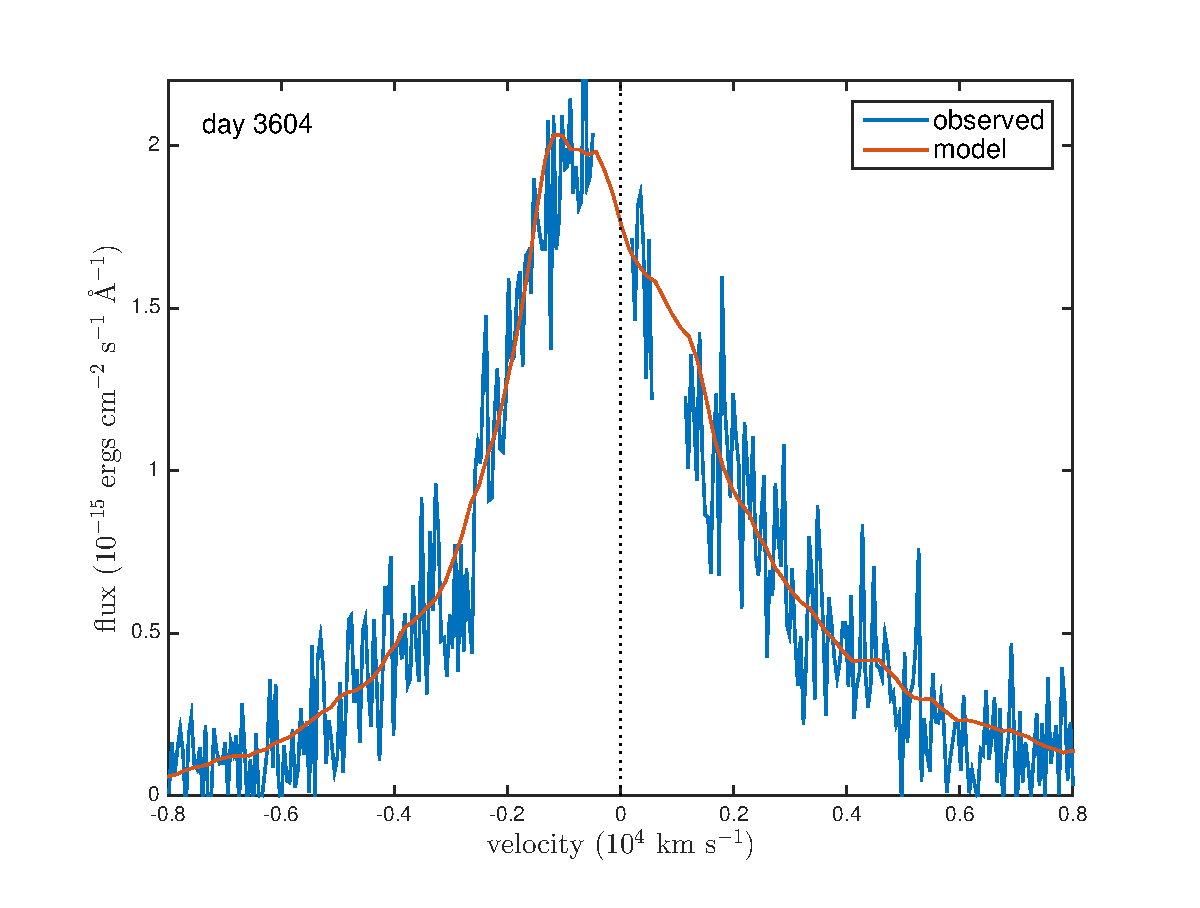
\includegraphics[trim =55 10 45 15,clip=true,scale=0.35]{smooth/best_fit/d3604Ha}
\caption{Best smooth model fit to the SN~1987A H$\alpha$ line at days 1862, 2875 and 
3604 for parameters detailed in Table \ref{smooth1} with amorphous carbon grains of radius $a=0.35 \mu$m.}
\label{d1862_3604}
\end{center}
\end{figure*}


There is rarely a unique set of parameters that provide the best fit to the data.  However, the 
majority of the parameters of interest can be well constrained from our 
modelling by considering different elements of the shape of the profile.  In particular, by constructing fits to 
the data using minimum and maximum limits for the grain 
size, credible lower and upper bounds on the possible dust mass formed 
within the ejecta may be derived.  We present here
 fits to the data obtained using both small and large values of the grain radius $a$ since it is the grain size which has the most significant effect on the overall 
dust mass required to reproduce the line profile (see Section \ref{params}).  

%We use pure amorphous carbon dust
All of our models are of a dusty medium composed solely of amorphous carbon grains. We use the optical 
constants from the BE sample presented in \citet{Zubko1996}.    Although previous SED modelling of SN~1987A has limited the fraction of silicates present in the dusty ejecta to a maximum of 15\% (\citet{Ercolano2007}, W15), it is useful to consider the effects on our models of using silicate dust.  We discuss this in detail in Section \ref{species}.

For each profile, the maximum velocity is identified from the data as the 
point where the emission vanishes on the blue side.  The equivalent point on 
the red side is indeterminate from observations due to the effects of 
dust scattering.  We determine the approximate value of $V_{min}$ by examining the width of the profile near its peak. It is unfortunate that the theoretical minimum velocity falls at 
a similar velocity to the 6583\AA\ line as any dust-induced features near this wavelength that would allow for more accurate determination of $V_{min}$
 will be overwhelmed by the nebular line.  Having determined the minimum and maximum velocities, the ratio 
of the inner and outer radii of the supernova ejecta may be determined since 
$R_{in}/R_{out}=V_{min}/V_{max}$.  The outer radius is calculated from the 
epoch and the maximum velocity.

The only parameters that then remain to be determined are the exponent of 
the density profile $\beta$, the mean grain  radius and the total dust mass.  The shape 
of the blue wing is solely a product of the density profile and the dust 
mass; the height and shape of the red wing is a product of these and also 
of the scattering efficiency of the grains (the albedo $\omega$); the 
extent and shape of the asymmetry in the flat-topped portion of the 
profile is a function of only the total dust optical depth determined by the 
dust mass and the grain radius.  By iterating over these three parameters 
therefore, an excellent fit to the data can usually be obtained.

Models are produced in the same manner for the 
[O~{\sc i}]~$\lambda$6300,6363~\AA\ doublet as for the single H$\alpha$ line, with each component 
of the doublet being modelled independently and the resulting profiles 
added according to a specified ratio.  Although the theoretical intrinsic flux ratio 
is 3.1 for optically thin emission, the actual ratio between the two components can be 
affected by self-absorption \citep{Li1992} and we therefore 
left it as a free parameter.  The deduced doublet ratios are listed in Tables \ref{smooth1}, \ref{clumped1} and \ref{clumped2}.  
%[O~{\sc i}] 
%$\lambda$6300,6363~\AA\ exhibits a clear blueshift as early as day 611 
%and provides another diagnostic for determining the dust mass.  By day 1862 
%the doublet is no longer strong enough to usefully 
%modelled (see Figure \ref{Ha_evol_early}).

For all lines, though particularly at very late epochs, even small fluctuations in the adopted value of the 
continuum level can have a substantial effect on the fit to the resulting 
profile.  Since it is not feasible to establish the level of the continuum 
so precisely, the value of the continuum has been left as a free parameter 
that may be adjusted (to within sensible margins) in order to allow for 
the widest possible dust mass range to be determined.  We generally find 
it is necessary to assume a continuum level that is slightly lower where 
the adopted dust mass is higher.  The [O~{\sc i}]$\lambda$6300,6363~\AA\ doublets at days 1054 and 1478 are weak relative to the continuum and are also blended with the wings of other lines making it difficult to fit their wings accurately.  We aim to fit the line between approximately -3000 km s$^{-1}$ and +5000 km s$^{-1}$ but present a wider velocity range for context (for example see Figure \ref{OI_smooth}).

Fits to the H$\alpha$ line profile at days 2211 and 3500 are omitted for the sake of space but are very similar in nature to those of days 1862 to 3604.  Parameters for the models at all epochs including these are detailed in Tables \ref{smooth1} to \ref{clumped2}.


\subsection{Smooth Density Models for SN 1987A}
\label{smooth_models}

Even at the earliest epochs there is a substantial wing on the red side of 
the H$\alpha$ line profile that cannot be fitted by scattering from moving grains with a low albedo.  The 
minimum required albedo is approximately $\omega \approx 0.5$ implying relatively large grain radii.  As previously discussed, the larger 
the grain size the larger the mass of dust required to reproduce the same 
optical depth.  Figure \ref{MRN} illustrates the 
a fit for the day 714 H$\alpha$ profile for the case where a classic MRN \citep{Mathis1977} grain size 
distribution is adopted, with $a_{min}=0.005 \mu m$, $a_{max}=0.25 \mu m$ 
and $n(a) \propto a^{-3.5}$.  It can be seen clearly that the extended red wing is 
significantly underestimated.  Since the albedo of  
amorphous carbon grains varies significantly with grain radius (see Figure \ref{albedo_grain}) we can establish a strong 
lower bound to the mean dust grain radius, which we estimate to be $a \ge 0.35\mu$m.  This is the smallest grain size that is still 
capable of reproducing the red scattering wing at all epochs and we 
therefore use this lower limit value throughout our smooth density modelling.

\begin{table*}
	\begin{minipage}{180mm}
	\caption{Details of the parameters used for the best fitting smooth models of SN~1987A with amorphous carbon grains of radius $a=0.35\mu$m.  Optical depths are given from $R_{in}$ to $R_{out}$.}
	\label{smooth1}
	\begin{center}
  	\begin{tabular}{@{} ccccccccccc @{}}
    	\hline
 & day & $V_{max}$ & $R_{in}/R_{out}$ & $\beta$ & $M_{dust}$ & $R_{out}$ & $R_{in}$ & [O~{\sc i}] ratio & $\tau_{H\alpha}$ & $\tau_V$  \\
	&& (km~s$^{-1} $) & & & ($M_{\odot}$) & (cm) & (cm) \\
	\hline
	%[O~{\sc i}]  & 714 & 5000 & 0.17 & 2.8 & 9.50$\times 10^{-5}$ &   3.08$\times 10^{15}$ & 5.24$\times 10^{15}$ & 2.9 & 1.09 & 2.19 & Fig. \ref{d714bf}\\ \relax
%[O~{\sc i}]  & 806 & 6000 & 0.15 & 2.7 & 1.60$\times 10^{-4}$ &   4.18$\times 10^{16}$ & 6.27$\times 10^{15}$ & 2.7 & 0.97 & 1.95 & Fig. \ref{d806bf} \\
[O~{\sc i}]  & 714 & 3250 & 0.07 & 2.9 & 1.15$\times 10^{-4}$ & 2.00$\times 10^{16}$ & 1.40$\times 10^{15}$ & 2.6 & 3.60 & 7.20  \\ \relax
[O~{\sc i}]  & 806 & 4000 & 0.06 & 2.4 & 1.80$\times 10^{-4}$ & 2.79$\times 10^{16}$ & 1.67$\times 10^{15}$ & 2.3 & 2.86 & 5.71  \\ \relax
[O~{\sc i}]  & 1054 & 4300 & 0.05 & 2.1 & 2.80$\times 10^{-4}$ &   3.92$\times 10^{16}$ & 1.96$\times 10^{15}$ & 2.7 & 2.23 & 4.45 \\ \relax
[O~{\sc i}]  & 1478 & 4500 & 0.04 & 1.7 & 3.50$\times 10^{-4}$ &   5.75$\times 10^{16}$ & 2.30$\times 10^{15}$ & 3.0 & 1.30 & 2.60 \\

H$\alpha$ & 714 & 3250 & 0.25 & 1.2 & 2.50$\times 10^{-5}$ &   2.00$\times 10^{16}$ & 5.01$\times 10^{15}$ & & 0.61 & 1.23 \\
%H$\alpha$ & 806 & 4500 & 0.25 & 1.8 & 3.00$\times 10^{-5}$ &   3.13$\times 10^{16}$ & 7.83$\times 10^{15}$ & & 0.30 & 0.60 \\
H$\alpha$ & 806 & 4000 & 0.22 & 1.9 & 4.50$\times 10^{-5}$ &   2.79$\times 10^{16}$ & 6.13$\times 10^{15}$ & & 0.52 & 1.05 \\
H$\alpha$ & 1862 & 8500 & 0.15 & 1.9 & 6.00$\times 10^{-4}$ &   1.37$\times 10^{17}$ & 2.05$\times 10^{16}$ & & 0.35 & 0.70\\
H$\alpha$ & 2211 & 9000 & 0.14 & 1.9 & 1.10$\times 10^{-3}$ &   1.72$\times 10^{17}$ & 2.41$\times 10^{16}$ & & 0.42 & 0.83\\
H$\alpha$ & 2875 & 9500 & 0.14 & 1.9 & 1.80$\times 10^{-3}$ &   2.36$\times 10^{17}$ & 3.30$\times 10^{16}$ & & 0.36 & 0.72 \\

H$\alpha$ & 3500 & 10000 & 0.14 & 1.9 & 4.00$\times 10^{-3}$  & 3.02$\times 10^{17}$ & 4.23$\times 10^{16}$ && 0.49 & 0.98  \\

H$\alpha$ & 3604 & 10250 & 0.13 & 1.9 & 5.00$\times 10^{-3}$ &   3.19$\times 10^{17}$ & 4.15$\times 10^{16}$ & & 0.55 & 1.10 \\ 

    \hline
  \end{tabular}
  \end{center}
\end{minipage}
\end{table*}


\begin{table*}
	\begin{minipage}{180mm}
	\caption{Details of the parameters used for the best fitting  clumped models of SN~1987A with amorphous carbon grains of radius $a=0.6\mu$m. Optical depths are given from $R_{in}$ to $R_{out}$.}
	\label{clumped1}
	\begin{center}
  	\begin{tabular}{@{} cccccccccccc @{}}
    	\hline
 & day & $V_{max}$ & $R_{in}/R_{out}$ & $\beta$ & $M_{dust}$ & $R_{out}$ & $R_{in}$ &  [O~{\sc i}] ratio & $\tau_{H\alpha}$ & $\tau_V$   \\
	&& (km~s$^{-1} $) & & & ($M_{\odot}$) & (cm) & (cm)   \\
	\hline
%[O~{\sc i}]  & 714 & 5000 & 0.17 & 2.8 & 2.70$\times 10^{-4}$ &   3.08$\times 10^{16}$ & 5.24$\times 10^{15}$ & 2.6 &  1.02 & 2.03 \relax
%[O~{\sc i}]  & 806 & 6000 & 0.15 & 2.7 & 6.00$\times 10^{-4}$ &   4.18$\times 10^{16}$ & 6.27$\times 10^{15}$ & 2.4 & 1.66 & 3.32 \\
[O~{\sc i}]  & 714 & 3250 & 0.07 & 2.7 & 4.50$\times 10^{-4}$ & 2.00$\times 10^{16}$ & 1.20$\times 10^{15}$ & 2.3 & 5.09 & 10.19  \\ \relax
[O~{\sc i}]  & 806 & 4000 & 0.06 & 2.3 & 7.00$\times 10^{-4}$ & 2.79$\times 10^{16}$ & 1.67$\times 10^{15}$ & 2.1 & 4.53 & 9.07 \\ \relax
[O~{\sc i}]  & 1054 & 4300 & 0.05 & 2.3 & 1.30$\times 10^{-3}$ &   3.92$\times 10^{16}$ & 1.96$\times 10^{15}$ & 2.3 & 4.33 & 8.67 \\ \relax
[O~{\sc i}]  & 1478 & 4500 & 0.04 & 2.0 & 1.60$\times 10^{-3}$ &   5.75$\times 10^{16}$ & 2.30$\times 10^{15}$ & 3.1 & 2.74 & 5.48 \\
%H$\alpha$ & 714 & 3250 & 0.25 & 1.2 & 7.00$\times 10^{-5}$ &   2.00$\times 10^{16}$ & 5.01$\times 10^{15}$ & & 0.87 & 1.74 \\
H$\alpha$ & 714 & 3250 & 0.25 & 1.4 & 7.00$\times 10^{-5}$ &   2.00$\times 10^{16}$ & 5.01$\times 10^{15}$ & & 0.87 & 1.74 \\
%H$\alpha$ & 806 & 4250 & 0.25 & 1.9 & 1.00$\times 10^{-4}$ &   2.96$\times 10^{16}$ & 7.40$\times 10^{15}$ & & 0.56 & 1.12\\
H$\alpha$ & 806 & 4000 & 0.22 & 1.8 & 1.20$\times 10^{-4}$ &   2.79$\times 10^{16}$ & 6.13$\times 10^{15}$ & & 0.79 & 1.59\\
H$\alpha$ & 1862 & 8500 & 0.14 & 1.9 & 1.65$\times 10^{-3}$ &   1.37$\times 10^{17}$ & 1.91$\times 10^{16}$ & & 0.48 & 0.96 \\

H$\alpha$ & 2211 & 9000 & 0.14 & 1.9 & 4.00$\times 10^{-3}$ &   1.72$\times 10^{17}$ & 2.41$\times 10^{16}$ & & 0.74 & 1.49\\

H$\alpha$ & 2875 & 9500 & 0.12 & 2 & 1.00$\times 10^{-2}$ &   2.36$\times 10^{17}$ & 2.83$\times 10^{16}$ & & 0.96 & 1.93 \\

H$\alpha$ & 3500 & 10000 & 0.12 & 2 & 1.80$\times 10^{-2}$  & 3.02$\times 10^{17}$ & 3.63$\times 10^{16}$ && 1.08 & 2.16  \\

H$\alpha$ & 3604 & 10250 & 0.12 & 2 & 2.30$\times 10^{-2}$ &   3.19$\times 10^{17}$ & 3.83$\times 10^{16}$ & & 1.21 & 2.42 \\ 

    \hline
  \end{tabular}
  \end{center}
\end{minipage}
\end{table*}



\begin{table*}
	\begin{minipage}{180mm}
	\caption{Details of the parameters used for the best fitting clumped models of SN~1987A with amorphous carbon grains of radius $a=3.5\mu$m. Optical depths are given from $R_{in}$ to $R_{out}$.}
	\label{clumped2}
	\begin{center}
  	\begin{tabular}{@{} ccccccccccccc @{}}
    	\hline
 & day & $V_{max}$ & $R_{in}/R_{out}$ & $\beta$ & $M_{dust}$  & $R_{out}$ & $R_{in}$ & [O~{\sc i}] ratio & $\tau_{H\alpha}$ & $\tau_V$\\
	&& (km~s$^{-1} $) & & & ($M_{\odot}$)  & (cm) & (cm)  \\
	\hline
	    %[O~{\sc i}]  & 714 & 5000 & 0.17 & 2.8 & 9.50$\times 10^{-5}$ &   3.08$\times 10^{16}$ & 5.24$\times 10^{15}$ & 2.9 & 1.09 & 2.19 & Fig. \ref{d714bf}\\ \relax
%[O~{\sc i}]  & 806 & 6000 & 0.15 & 2.7 & 1.60$\times 10^{-4}$ &   4.18$\times 10^{16}$ & 6.27$\times 10^{15}$ & 2.7 & 0.97 & 1.95 & Fig. \ref{d806bf} \\
[O~{\sc i}]  & 714 & 3250 & 0.07 & 2.9 & 3.50$\times 10^{-3}$ & 2.00$\times 10^{16}$ & 1.40$\times 10^{15}$ & 2.5 & 5.32 & 10.64  \\ \relax
[O~{\sc i}]  & 806 & 4000 & 0.06 & 2.3 & 5.00$\times 10^{-3}$ & 2.79$\times 10^{16}$ & 1.67$\times 10^{15}$ & 2.1 & 4.72 & 9.45  \\ \relax
[O~{\sc i}]  & 1054 & 4300 & 0.05 & 2.3 & 8.00$\times 10^{-3}$ &   3.92$\times 10^{16}$ & 1.96$\times 10^{15}$ & 2.5 & 3.89 & 7.78 \\ \relax
[O~{\sc i}]  & 1478 & 4500 & 0.04 & 1.9 & 1.10$\times 10^{-2}$ &   5.75$\times 10^{16}$ & 2.30$\times 10^{17}$ & 2.8 & 2.77 & 5.54 \\
H$\alpha$ & 1862 & 8500 & 0.14 & 1.9 & 2.00$\times 10^{-2}$  & 1.37$\times 10^{17}$ & 1.91$\times 10^{16}$ && 0.85 & 1.70  \\

H$\alpha$ & 2211 & 9000 & 0.14 & 1.9 & 3.30$\times 10^{-2}$ &   1.72$\times 10^{17}$ & 2.41$\times 10^{16}$ & & 0.89 & 1.78\\

H$\alpha$ & 2875 & 9500 & 0.12 & 2 & 8.00$\times 10^{-2}$  & 2.36$\times 10^{17}$ & 2.83$\times 10^{16}$ && 1.15 & 2.30  \\

H$\alpha$ & 3500 & 10000 & 0.12 & 2 & 1.50$\times 10^{-1}$  & 3.02$\times 10^{17}$ & 3.63$\times 10^{16}$ && 1.31 & 2.62  \\

H$\alpha$ & 3604 & 10250 & 0.12 & 2 & 1.70$\times 10^{-1}$  & 3.19$\times 10^{17}$ & 3.83$\times 10^{16}$ && 1.33 & 2.67  \\ 

    \hline
  \end{tabular}
  \end{center}
\end{minipage}
\end{table*}


The ejecta inner and outer radii are calculated at each epoch from the maximum 
velocity used, the day number and the specified ratio $R_{in}/R_{out}$.  
The radii generated are consistent with those used in previous models of 
SN 1987A \citep{Ercolano2007, Wesson2015}.  Figures \ref{Ha_smooth} to 
\ref{d1862_3604} show the best fits to the data for days 714 to 3604 whilst 
Table \ref{smooth1} details the parameters used.

It can be seen from Tables \ref{smooth1} to \ref{clumped2} that, in order to reproduce the blueshifts seen in the 
[O~{\sc i}]~$\lambda$6300,6363~\AA\ doublet, considerably larger dust masses 
are required than to fit the H$\alpha$ line at the same epoch.  Although the same maximum velocities and therefore outer radii are used in our [O~{\sc i}] and H$\alpha$ models, the inner radii for the [O~{\sc i}] models are significantly smaller and the density distribution much steeper.  This implies that the [O~{\sc i}] is concentrated towards the centre of the ejecta whereas the H$\alpha$ is more diffuse.  This is broadly in agreement with 3D explosion dynamics models that suggest that a few hours after the explosion the heavier elements will, in comparison to H{\sc i}, be located more centrally in the ejecta with ``bullets" of heavier material reaching the outer edges  \citep{Hammer2010}.  If dust is forming in the inner regions of the ejecta then the majority of the  [O~{\sc i}] emission must travel through the newly formed dust whereas the more diffuse H$\alpha$ emission has a greater chance of escaping unaffected.  This may explain the difference between the dust masses needed for the [O~{\sc i}] and H$\alpha$ models.


%However, larger maximum 
%velocities are also required to fit the wings and a significantly steeper 
%density profile is required.  The inner radii remain approximately similar 
%in both the H$\alpha$ and [O~{\sc i}]~$\lambda$6300,6363~\AA\ models whilst the 
%outer radii are significantly different.  This may indicate why a greater 
%dust mass is required in order to fit the [O~{\sc i}] doublet; the doublet may
%trace the dust to a wider radius than the H$\alpha$ line at these epochs.


\subsection{Clumped Models for SN 1987A}
\label{clumped_models}


It has been shown through the modelling of optical-IR SEDs that when dust 
is assumed to have a clumped distribution the derived dust masses can be 
significantly larger than if the dust is distributed smoothly between the 
inner and outer radii (e.g. \citet{Owen2015}).  We present two sets of fits to the line profile based on 
the clumped dust modelling of W15, one set with a minimum grain size and one set with a maximum grain size.  Each fit is based on the best 
fitting smooth model such that the photon packets are emitted assuming a smooth 
radial density profile.  However, the dust is no longer coupled to the gas 
but instead is located entirely in clumps of size $R_{out}/50$.  The 
clumps are distributed stochastically between $R_{in}$ and $R_{out}$ with 
the probability of a given grid cell being a clump proportional to $r^{- 
\beta }$ where $i(r) \propto r^{-2 \beta}$.  The number of clumps used is 
determined by the clump filling factor $f$ which is kept constant at $f=0.1$.  All 
properties are fixed from the smooth models with the exception of the grain 
radius, density profile exponent ($\beta$) and the total dust mass.


Models were again constructed using the smallest possible grain radius (a=0.6 $\mu$m in the clumped case) in order to derive minimum dust masses for clumped distributions.  By considering the extent of the red scattering wing, upper limits to the grain size were also derived with the purpose of limiting the maximum  dust mass at each epoch.  By 
steadily reducing the grain radius from an initial value of 5$\mu$m 
(motivated by the maximum possible grain size derived by W15 for their day 
8515 model), we produced a set of models with a maximum grain radius of $a=3.5\mu$m.  

For all but the H$\alpha$ line at days 714 and 806 a similar fit could be obtained with either a grain radius of $a=0.6\mu$m or $a=3.5\mu$m (see Figures \ref{Ha_clump1} to 
\ref{d1862_3604_cmax}).  However, for H$\alpha$ at days 714 and 806  even a small change to the grain radius resulted in a significantly poorer fit, either 
over- or under-estimating the red wing. We therefore conclude that the dust mass estimates produced for the H$\alpha$ lines at days 714 and 
806 for a grain radius of $a=0.6\mu$m are the best H$\alpha$-based estimates of the dust mass 
at this epoch.  Details of the parameters used in all clumped models are
presented in Tables \ref{clumped1} and \ref{clumped2} and fits are presented in Figures \ref{Ha_clump1} to \ref{d1862_3604_cmax}.

In our subsequent analyses, we adopt the values derived from our clumped models.  The location of dust in clumps is thought to be a more likely scenario supported by the expectation of Rayleigh-Taylor instabilities and macroscopic mixing in the ejecta \cite{Ercolano2007,Hammer2010}.

%Throughout the course of our modelling it transpired that the 
%grain size used for the minimum H$\alpha$ models at days 714 and 806 ($a=0.6\mu$m) 
%in fact represents the best fit to the data and   

%At much later epochs (days 1862 - 3604) for H$\alpha$ and for all epochs modelled for [O~{\sc i}] we find that equally good fits may 
%be generated by substantially larger grains, with grain radii up to $a=3.5\mu$m 


 \begin{figure*}
\begin{center}
\includegraphics[trim =33 10 45 15,clip=true,scale=0.47]{clump_1/best_fit/d714Ha_new}
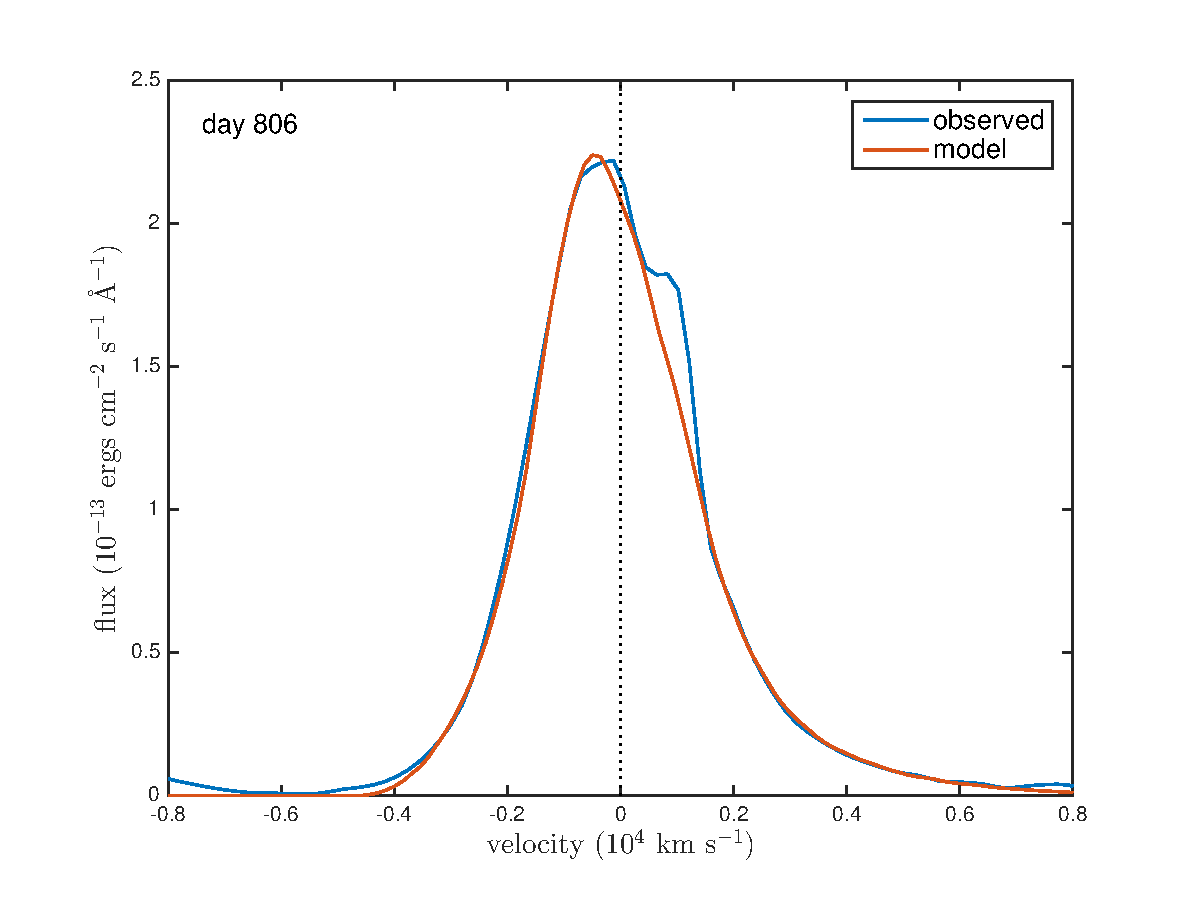
\includegraphics[trim =33 10 45 15,clip=true,scale=0.47]{clump_1/best_fit/d806Ha_new}
\caption{Best clumped dust fit to the SN~1987A H$\alpha$ line at day 714 \textit{\textit{(left)}} and day 806 \textit{\textit{(right)}} for the parameters detailed in Table \ref{clumped1} with amorphous carbon grains of radius $a=0.6 \mu$m.}
\label{Ha_clump1}
\end{center}
\end{figure*}
\begin{figure*}
\begin{center}
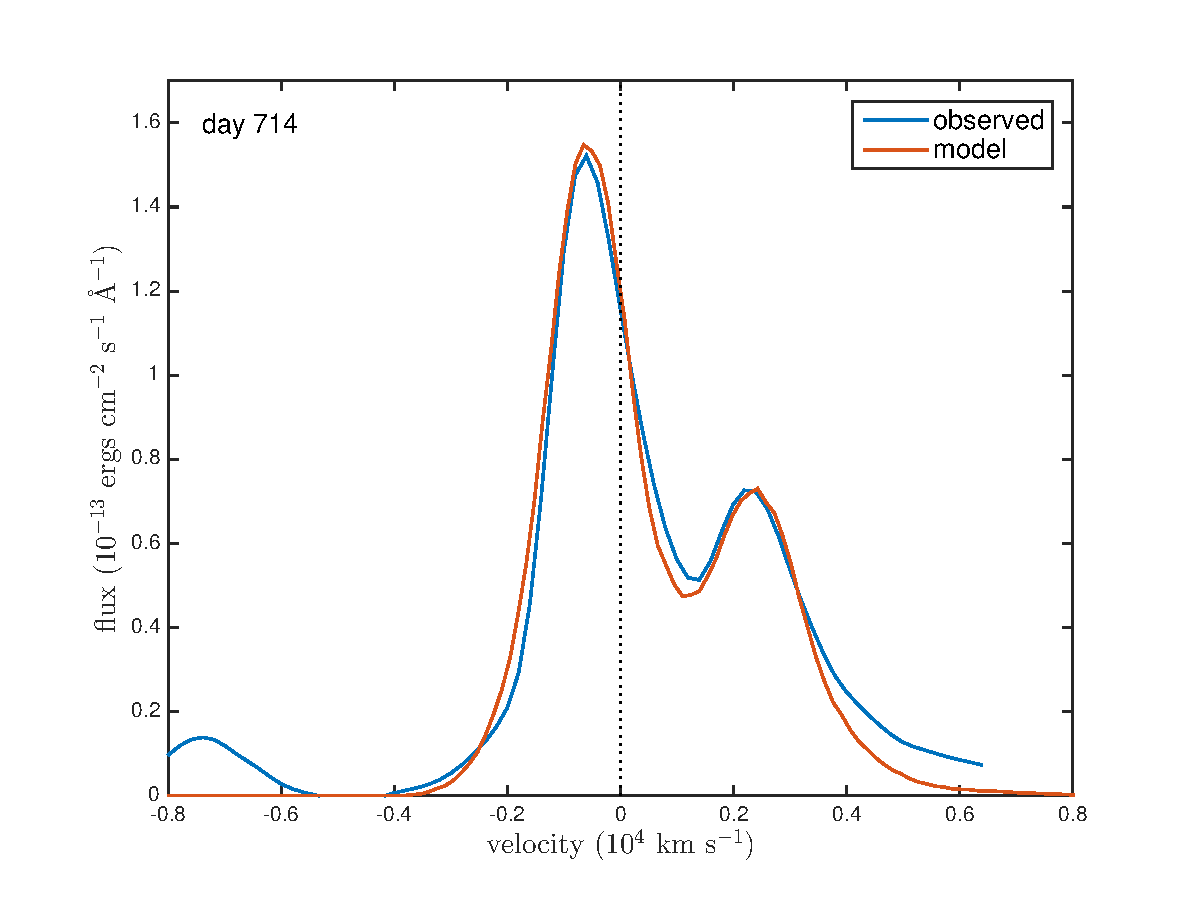
\includegraphics[trim =33 10 45 15,clip=true,scale=0.47]{clump_1/best_fit/d714OI_new}
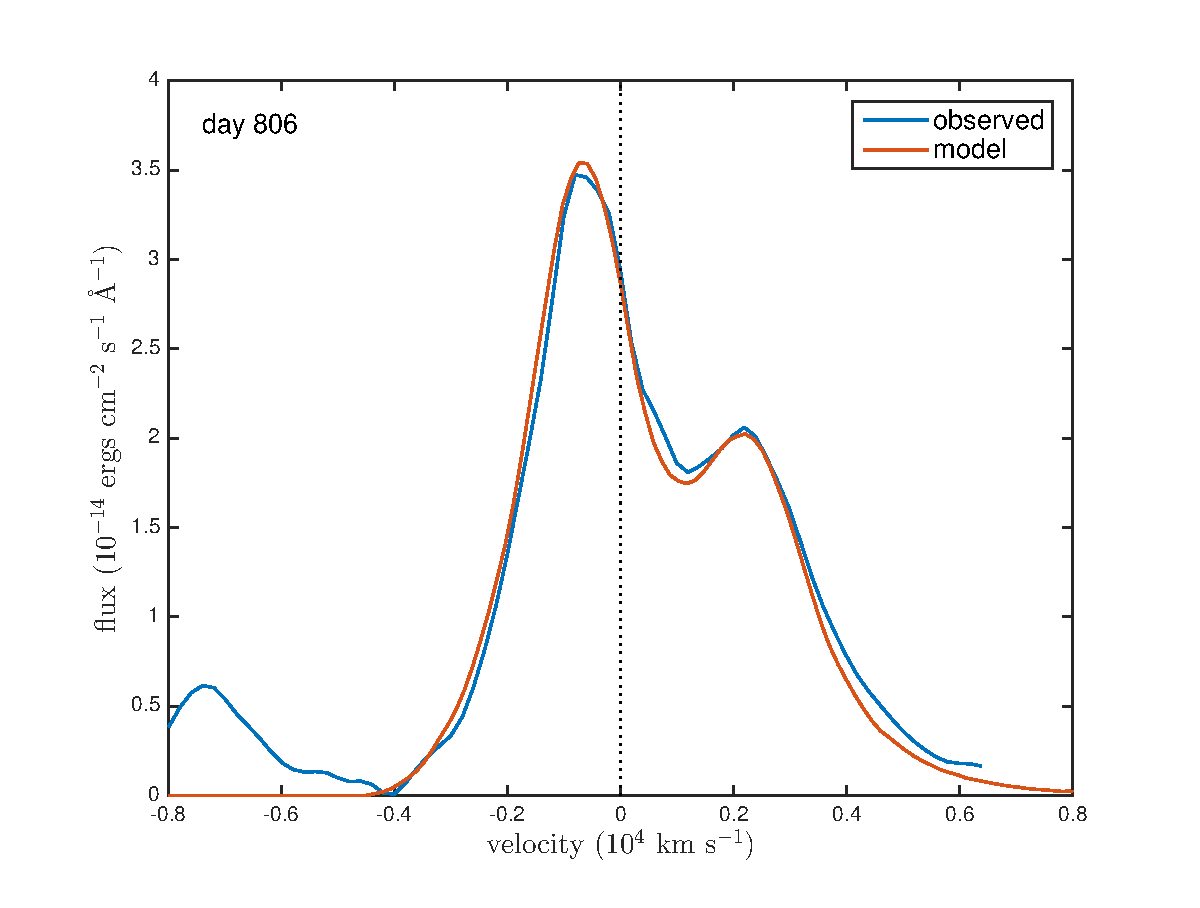
\includegraphics[trim =33 10 45 15,clip=true,scale=0.47]{clump_1/best_fit/d806OI_new}
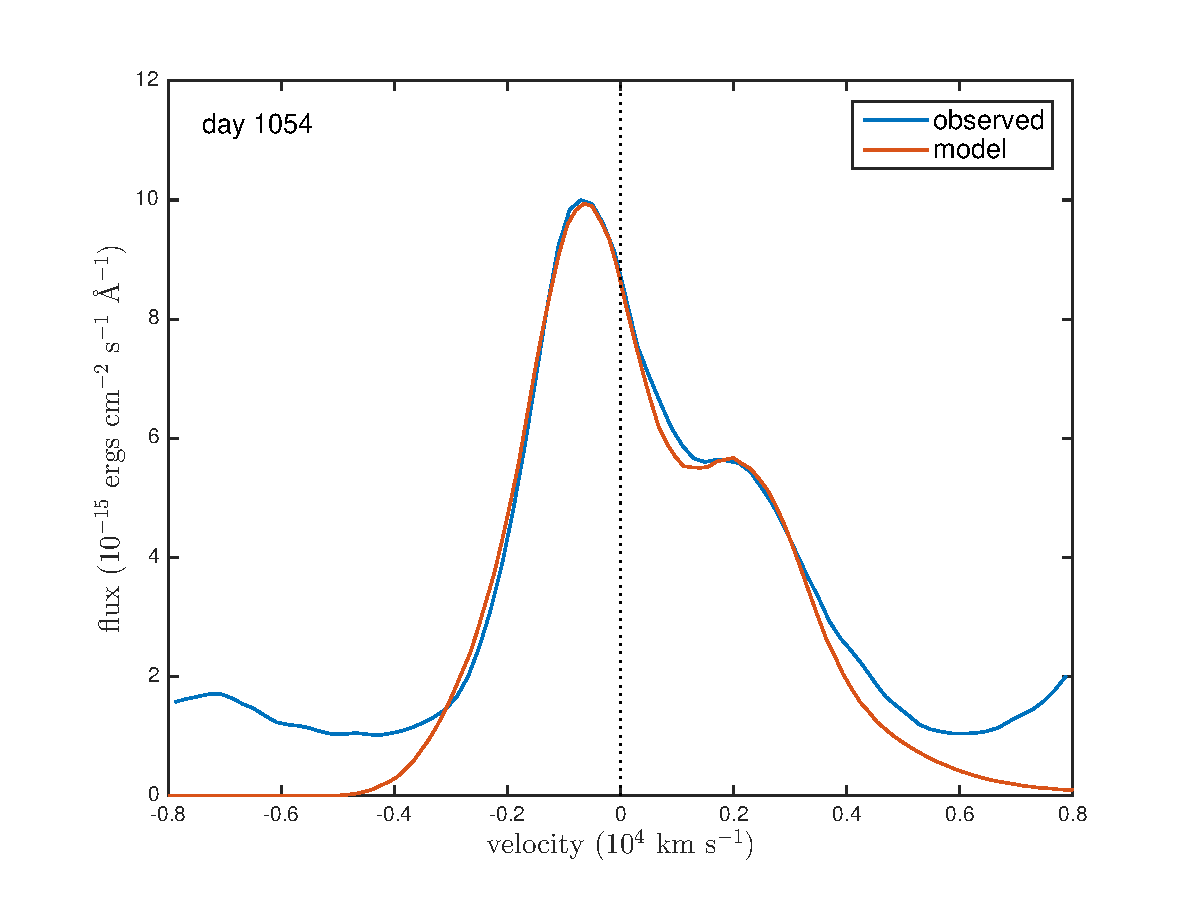
\includegraphics[trim =33 10 45 15,clip=true,scale=0.47]{clump_1/best_fit/d1054OI}
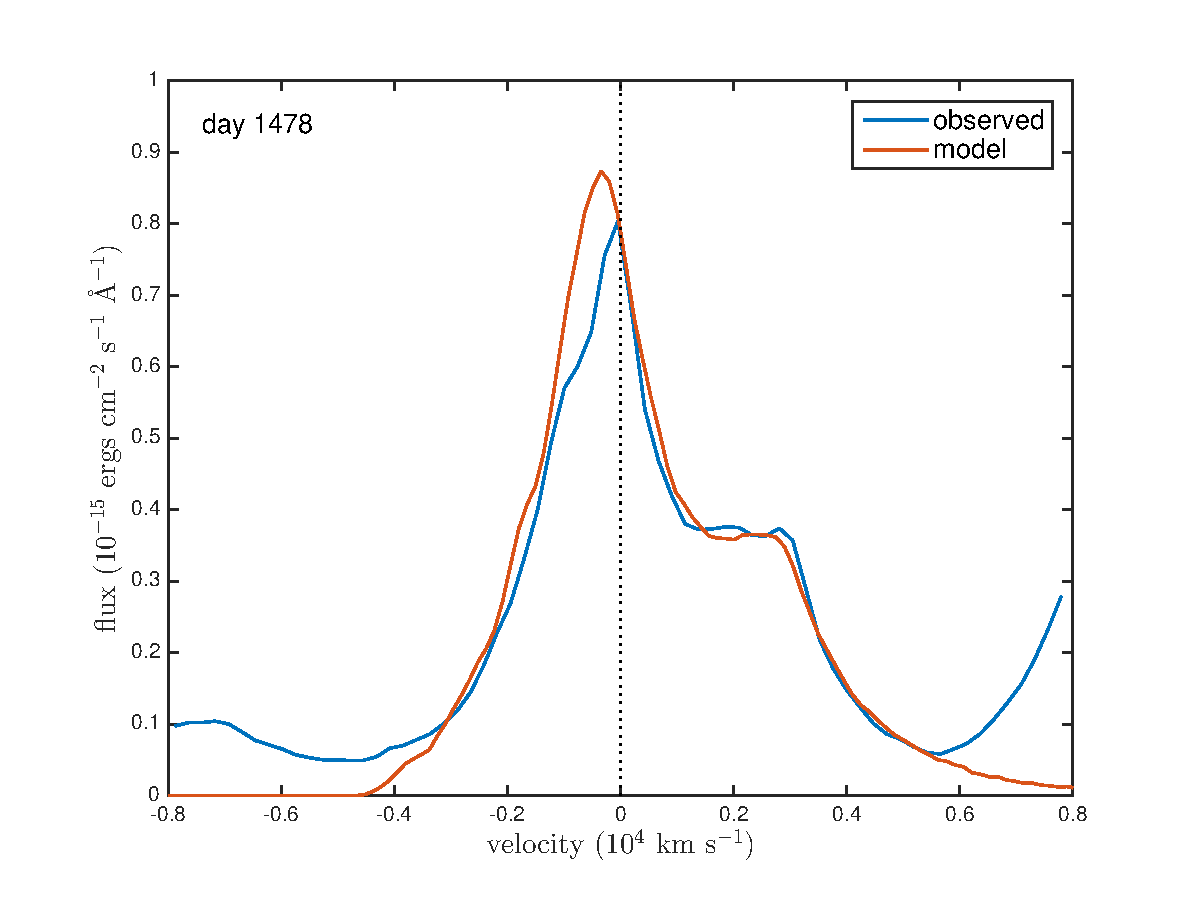
\includegraphics[trim =33 10 45 15,clip=true,scale=0.47]{clump_1/best_fit/d1478OI}
\caption{Best clumped dust fit to the SN~1987A [O~{\sc i}]~$\lambda$6300,6363~\AA\ doublet at day 714 \textit{(upper left)}, day 806 \textit{(upper right)}, day 1054 \textit{(lower left)} and day 1478 \textit{(lower right)} for the parameters detailed in Table \ref{clumped1} with amorphous carbon grains of radius $a=0.6 \mu$m.}
\label{OI_clump1}
\end{center}
\end{figure*}

\begin{figure*}

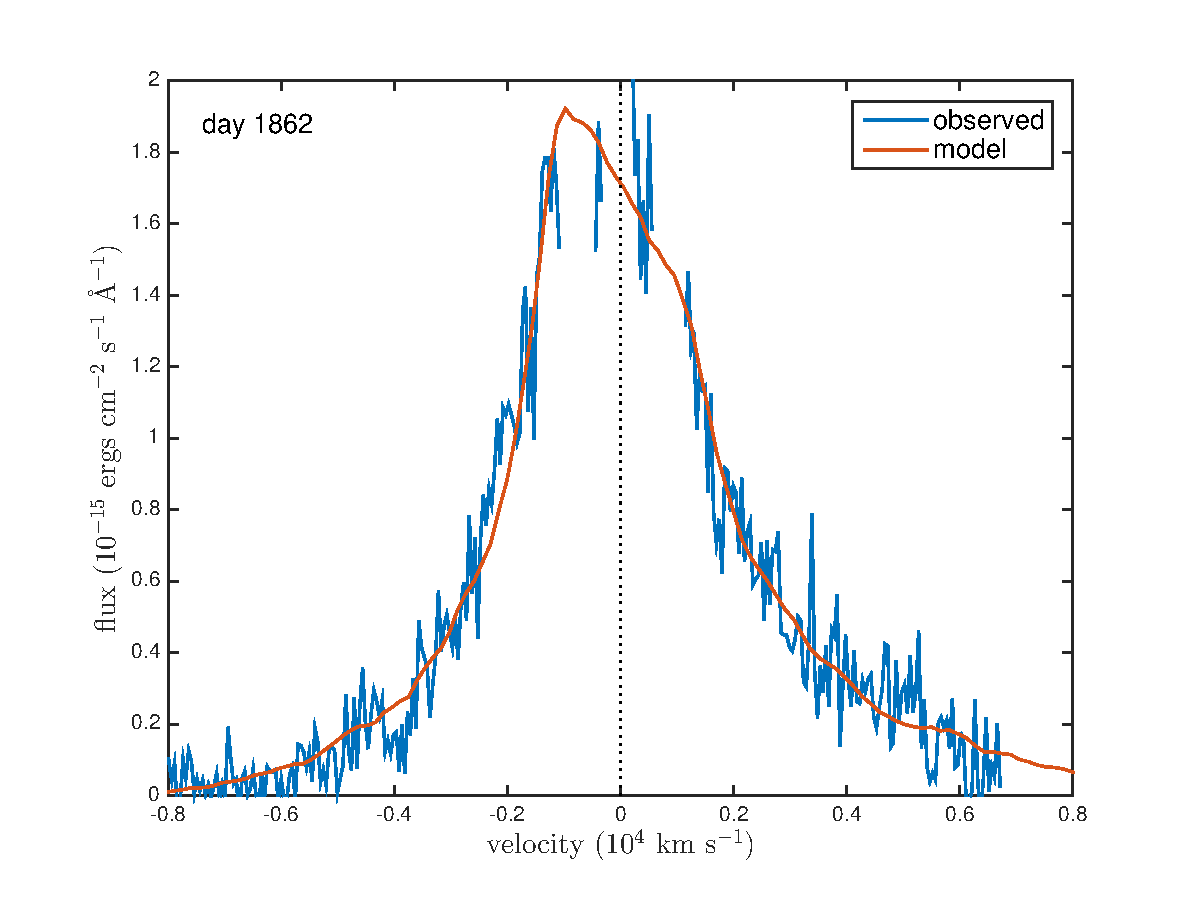
\includegraphics[trim =33 10 45 15,clip=true,scale=0.35]{clump_1/best_fit/d1862Ha}
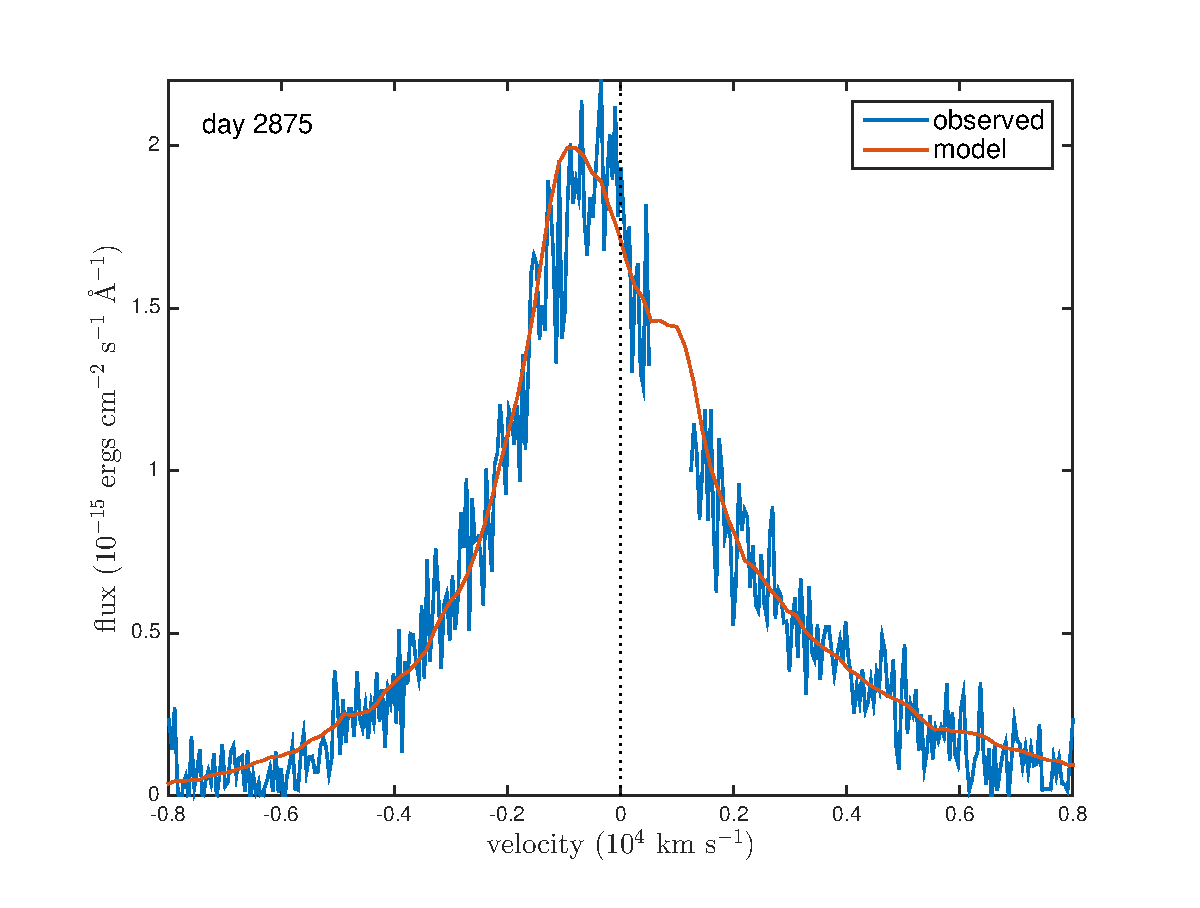
\includegraphics[trim =55 10 45 15,clip=true,scale=0.35]{clump_1/best_fit/d2875Ha}
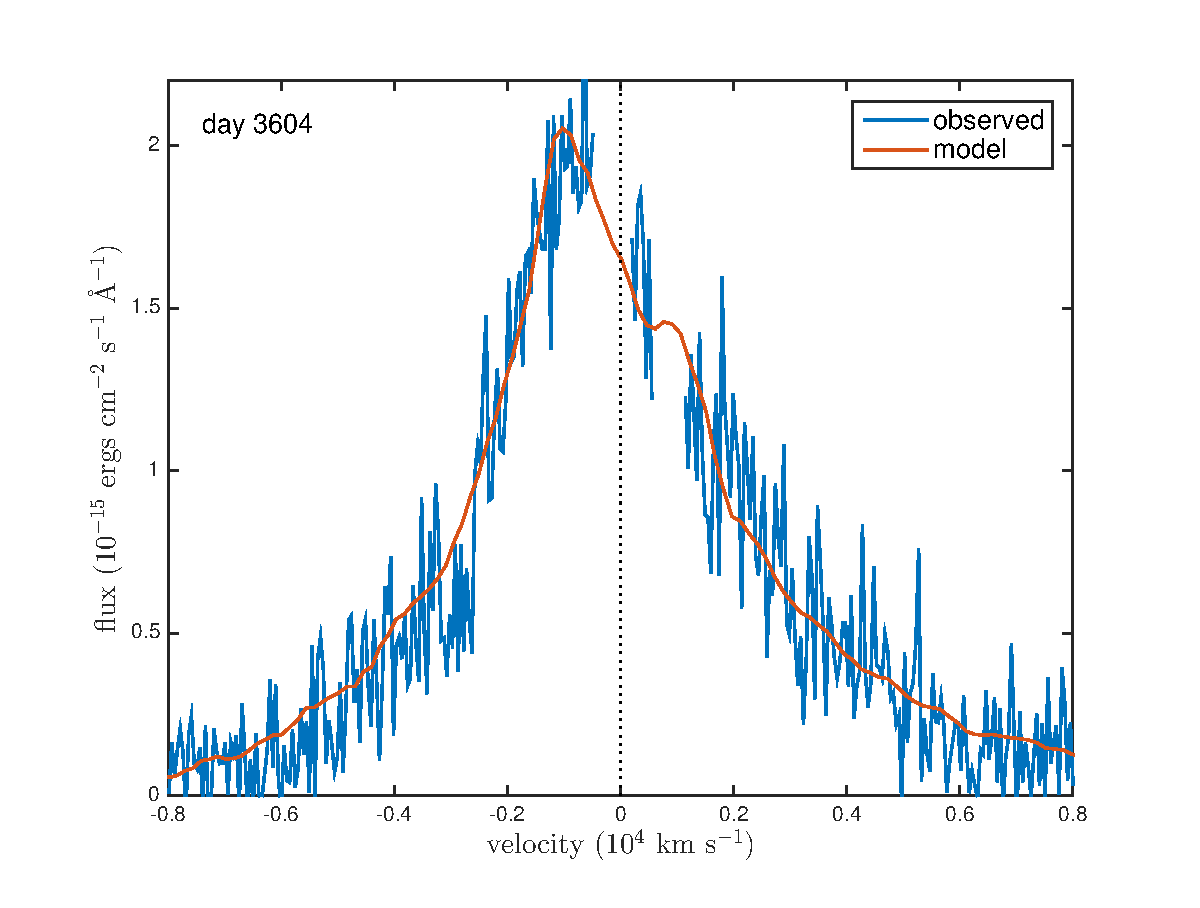
\includegraphics[trim =55 10 45 15,clip=true,scale=0.35]{clump_1/best_fit/d3604Ha}
\caption{Best clumped dust fit to the SN~1987A  H$\alpha$ line at days 1862, 2875 and 
3604 for the parameters detailed in Table \ref{clumped1} with amorphous carbon grains of radius $a=0.6\mu$m.}
\label{d1862_3604_c}

\end{figure*}

\subsection{The effect of clumping}


As in the case of SED radiative transfer models, the dust masses required to reproduce the 
observations in the clumped scenario are considerably higher than for the smooth scenario.  The dust masses differ between our smooth models for $a=0.35\mu$m and clumped models for $a=0.6\mu$m by a factor of approximately 3.  This does not take into account the increase in grain radius between the two cases however.  This increase accounts for a reasonable fraction of this difference. We estimate the effects of clumping alone to increase the required dust mass by a factor of approximately 1.5-2.0 from the smooth case.

The increase in grain size from the smooth case to the clumped case is necessary in order to have a slightly larger albedo.  Grains of radius $a=0.35 \mu$m do not reproduce the red side of the profiles well for a clumped medium.  This is because when 
the dust is located in clumps the radiation is subject to less scattering 
as well as to less absorption.  The reduction in scattering appears not to be 
compensated for by the increased dust mass and a larger grain radius is 
therefore required, particularly at day 714.  A grain radius of $a=0.6\mu$m 
is therefore used throughout the clumped models as the smallest possible 
grain size capable of reproducing the observed profiles, although this still underestimates the red wing in some instances. 



%%%%%%%ADDITIONAL CONTENT%%%%%%%%%%%%%%%%%

\subsection{The effect of a grain size distribution}
\label{gs_distn}
It is important to consider the potential effect on the dust mass of modelling a grain size distribution instead of a single grain size.  For a grain size distribution the overall extinction cross section, $C_{ext}$, at a given wavelength is 

\begin{equation}
 C_{ext}=\int^{a_{max}}_{a_{min}} Q_{ext}(a) n(a) \pi a^2 da 
 \end{equation}

where $Q_{ext}(a)$ is the extinction efficiency for a grain size $a$ and $n(a)$ is the number of grains with size $a$. The overall extinction efficiency is then

\begin{equation}
 Q_{ext} = \frac{C_{ext}}{ \int^{a_{max}}_{a_{min}} n(a) \pi a^2 da} 
 \end{equation}
 
 


 
The scattering cross-section $Q_{sca}$ is similarly calculated.  As a result of these calculations, there is rarely a single grain size that has the same albedo and extinction efficiency as a size distribution.  Modelling a size distribution may therefore alter the deduced dust mass.  Since the models are only sensitive to the overall optical depth and albedo, it is not possible to deduce the grain size range or distribution and only single grain sizes are investigated (as presented above).

Whilst this apparently limits the scope of the results, it is useful to consider the extent to which considering grain size distributions would alter the derived dust masses.  By considering a number of grain radius ranges and adopting a power law distribution with a variable exponent, we may gain some insight into the effects of adopting a distribution rather than a single size.  For the classical MRN power law ($n(a) \propto a^{-3.5}$) with a wide grain radius range ($a_{min} = 0.001 \mu$m to $a_{max} = 4.0 \mu$m) the derived albedo is much too small to reproduce the required wing seen at early epochs.  We therefore adopt an approach whereby, for a number of grain size ranges, we adjust the exponent of the distribution until the overall albedo is the same as that seen for the best fitting single grain radius for the clumped distributions.  We may then approximately calculate the required dust mass as

\begin{equation}
\label{distn_conv}
M_{d}= \frac{M_s Q_{ext,s}(a_s)}{a_s} \times \frac{\int^{a_{max}}_{a_{min}} n(a) a^3 da}{\int^{a_{max}}_{a_{min}} Q_{ext}(a) n(a) a^2 da}
\end{equation}

where the subscript $s$ represents the single grain size quantities and the $d$ subscript represents quantities for the grain size distribution.  


\begin{figure*}
\begin{center}
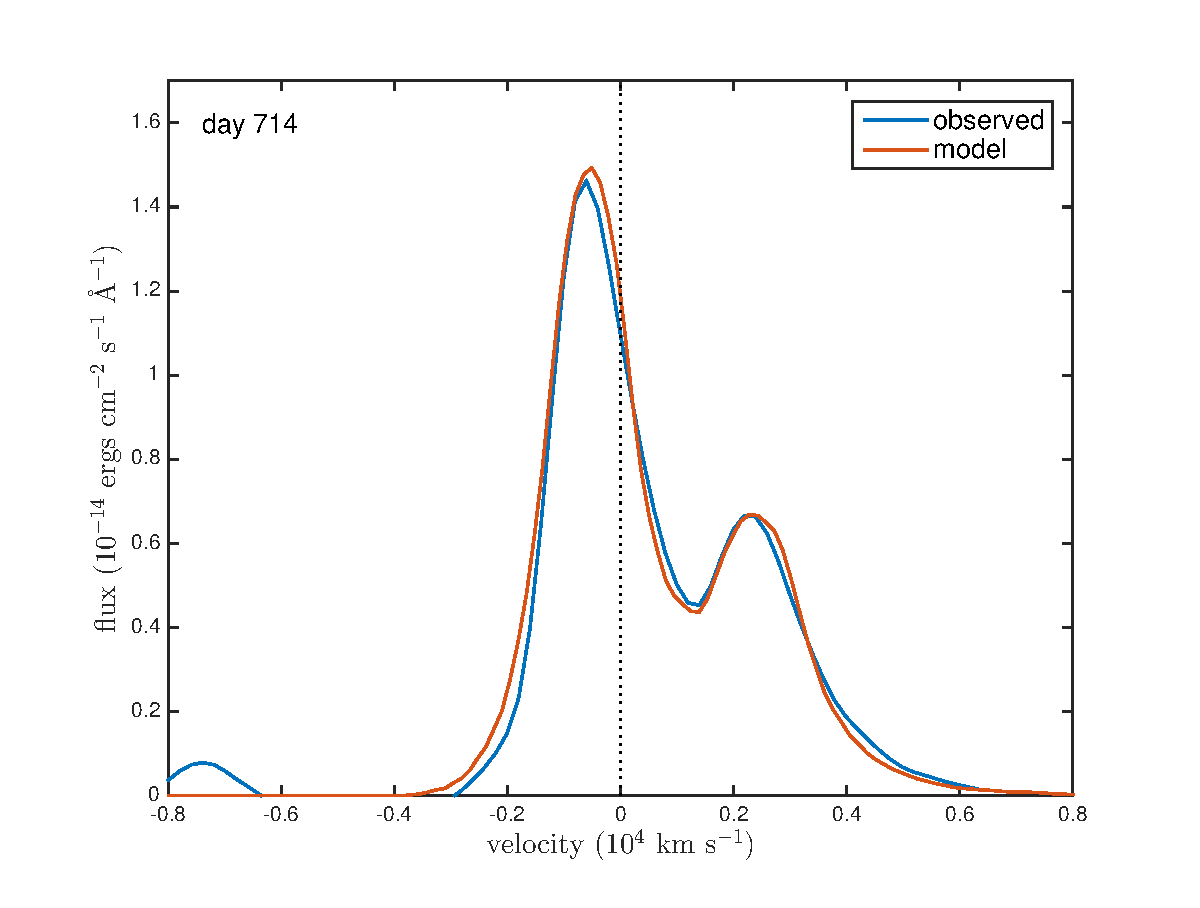
\includegraphics[trim =33 10 45 15,clip=true,scale=0.47]{clump_1/maximum/d714OI}
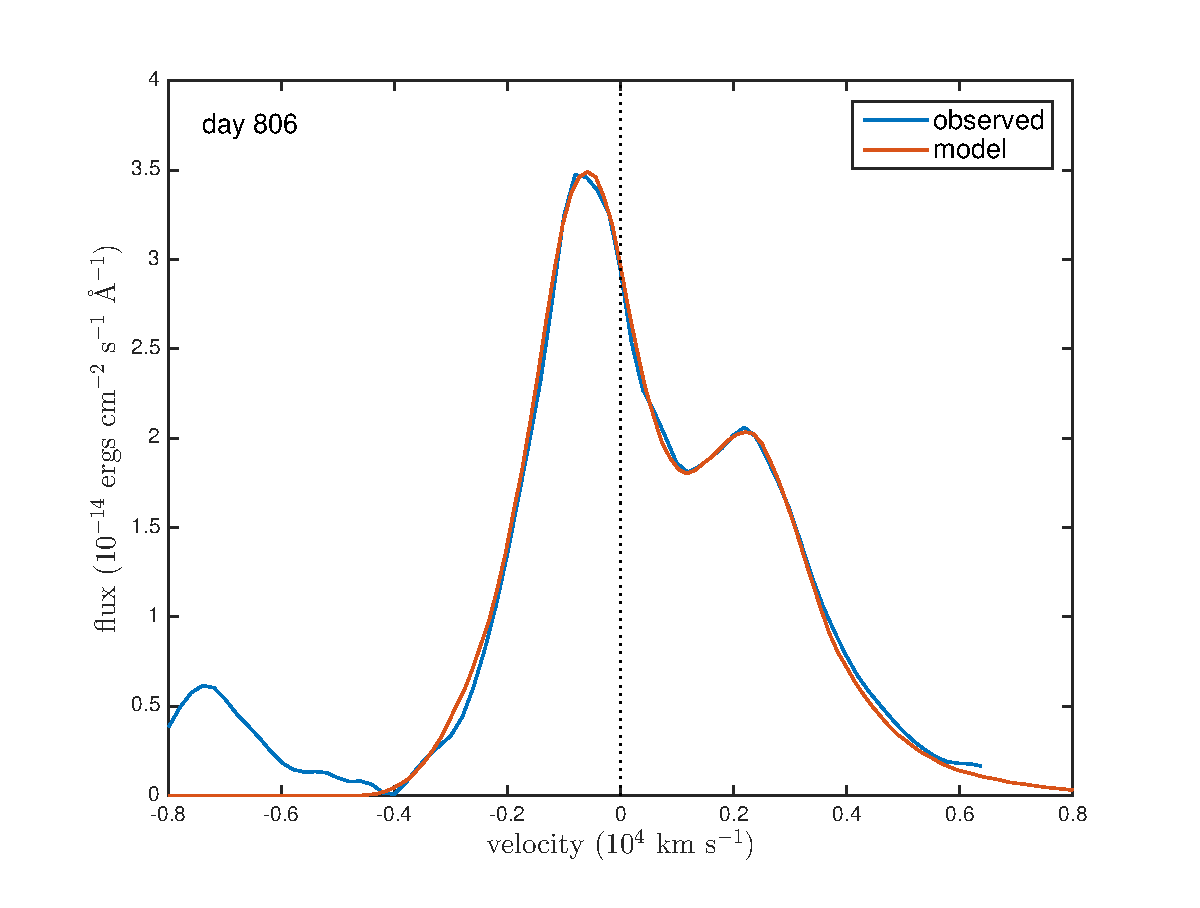
\includegraphics[trim =33 10 45 15,clip=true,scale=0.47]{clump_1/maximum/d806OI}
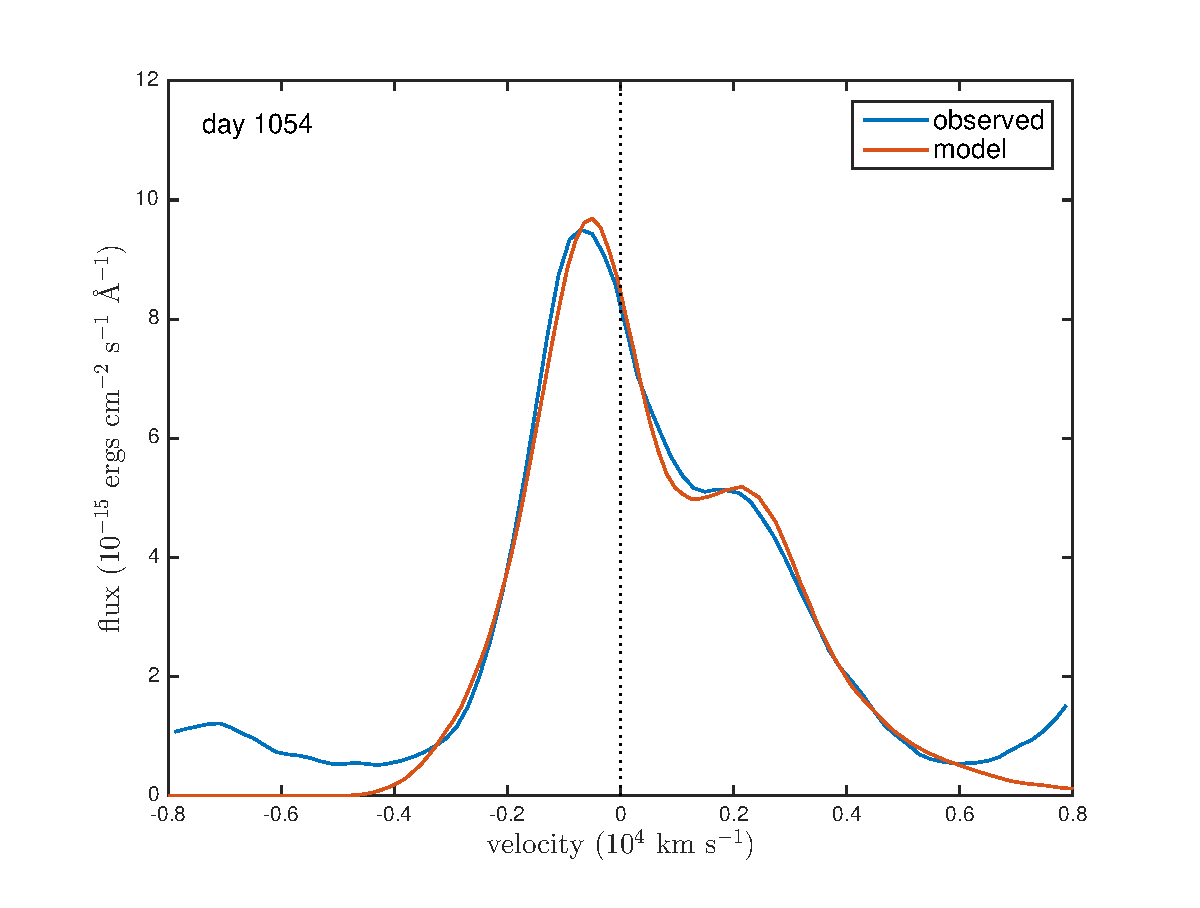
\includegraphics[trim =33 10 45 15,clip=true,scale=0.47]{clump_1/maximum/d1054OI}
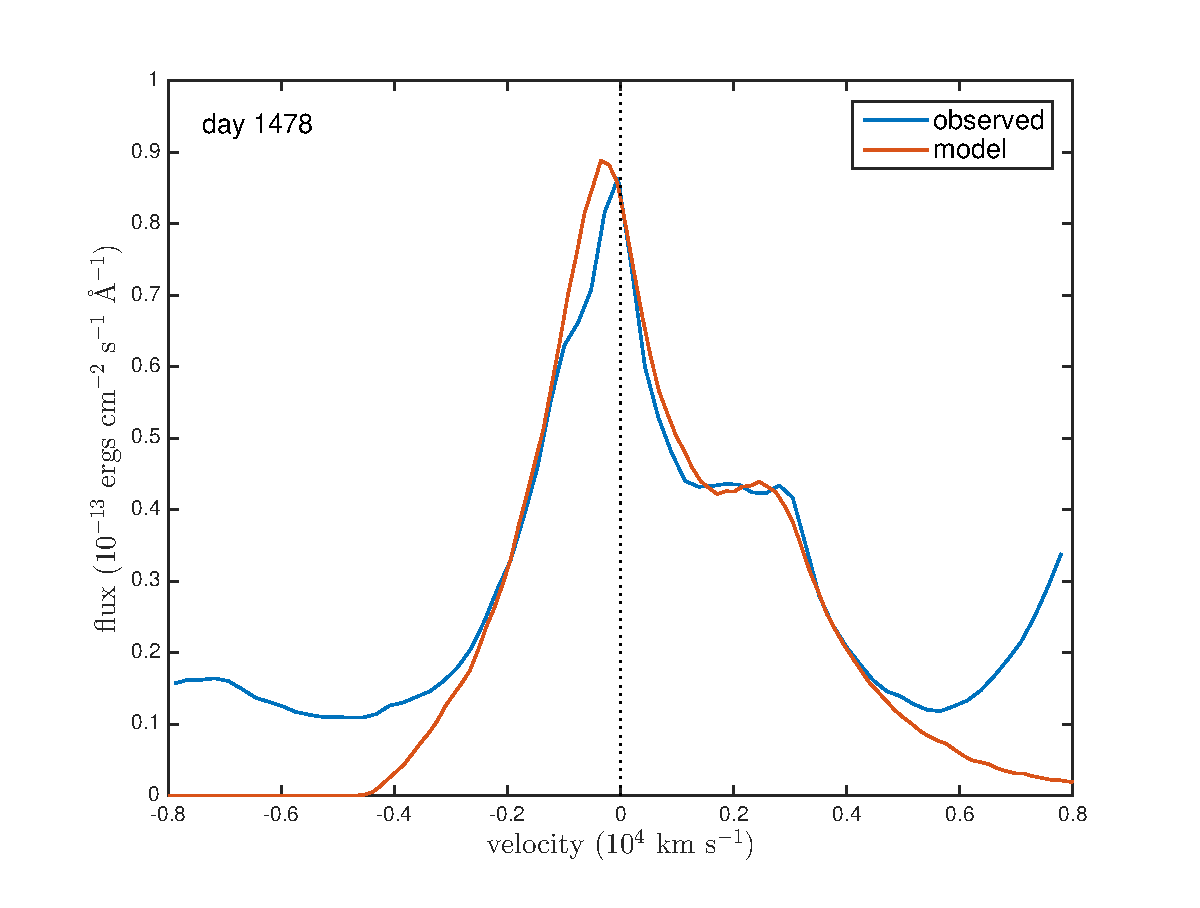
\includegraphics[trim =33 10 45 15,clip=true,scale=0.47]{clump_1/maximum/d1478OI}
\caption{Best clumped dust fit to the SN~1987A [O~{\sc i}]~$\lambda$6300,6363~\AA\ doublet at day 714 \textit{(upper left)}, day 806 \textit{(upper right)}, day 1054 \textit{(lower left)} and day 1478 \textit{(lower right)} for the parameters detailed in Table \ref{clumped2} with amorphous carbon grains of radius $a=3.5 \mu$m.}
\label{OI_clump2}
\end{center}
\end{figure*}

We calculate the required dust masses for the clumped H$\alpha$ model on day 714 for a selection of distributions with varying $a_{min}$.  These are presented in Table \ref{tb_distn}.  It can be seen that in all cases, a larger dust mass is required in order to reproduce the same profile as a single grain size.  The conversion factors presented in the table are valid for any model with grain size $a=0.6\mu$m and may therefore also be applied to the models for day 806.  We repeated the process for $a=3.5 \mu$m but found that, in order to reproduce the required albedo, the distribution had to be heavily weighted towards the larger grains and that the value of $a_{min}$ had no effect on the required dust mass.  Increasing the value of $a_{min}$ to larger values ($>2\mu$m) does not have a significant effect either.  This is because both extinction efficiency and albedo tend to a constant value with increasing grain radius and the adoption of different grain size ranges and distributions above a certain threshold results in only insignificant variations in these quantities. 



\begin{table}
	%\begin{minipage}{180mm}
	\caption{Dust masses for day 714 clumped models of the H$\alpha$ line using different grain size distributions and 100\% amorphous carbon. $f$ is factor of increase over the dust mass for the single size model ($M=7 \times 10^{-5} M_{\odot}$ with $a=0.6 \mu$m) and $p$ is the exponent of the grain size distribution $n(a) \propto a^{-p}$.}
	\label{tb_distn}
	\begin{center}
  	\begin{tabular}{@{} ccccc @{}}
    	\hline
$a_{min}$ & $a_{max}$ & $p$ & $M$ & $f$  \\%& $Q_{ext}$ \\
($\mu$m) & ($\mu$m) & & ($M_{\odot}$) & \\
\hline
0.001 & 4.0 & 2.45 & 1.93 $\times 10^{-4}$ & 2.76 \\%& 2.13 \\
0.01 & 4.0 & 2.45 & 1.93 $\times 10^{-4}$ & 2.76 \\%& 2.32 \\
0.05 & 4.0 & 2.52 & 1.84 $\times 10^{-4}$ & 2.62 \\%& 2.44 \\
0.1 & 4.0 & 2.72 & 1.61 $\times 10^{-4}$ & 2.3\\ %& 2.53 \\
0.5 & 4.0 & 8.20 & 7.23 $\times 10^{-5}$ & 1.03 \\%& 2.61 \\

    \hline
  \end{tabular}
  \end{center}
%\end{minipage}
\end{table}

Equation \ref{distn_conv} holds only for a single wavelength and therefore is not exact for our models, which transport radiation over a range of wavelengths.  However, the dust masses derived using the above formula produce almost identical fits to the data as for the single grain size case and therefore should give a good representation of the dust mass required when using a distribution.

We  conclude that if a distribution of grain sizes is indeed present, the deduced dust masses are likely to  under-estimate the true mass of newly formed dust.



\subsection{The effect of different grain species}
\label{species}
In  our analyses so far we have considered only amorphous carbon as the species of interest.  This is motivated by previously published optical and IR analyses that have found that if silicates contribute a fraction of the total dust mass, this fraction is limited to approximately 15\% or less (\citet{Ercolano2007}, W15).  The parameters that affect the quantity of dust required by our models here are the mean albedo and  optical depth of the dust.  There could be multiple combinations of grain species and sizes that result in a good fit to the data.  

We can consider the change in dust mass when a medium of 100\% silicates is used instead of amorphous carbon, using the astronomical silicate optical constants presented by \cite{Draine1984}.  In a similar manner to the approach detailed in Section \ref{gs_distn}, we  calculated the mass of silicates that gives a fit equivalent to that for a single carbon grain size.  We consider the albedo for the original carbon grain size, calculate the equivalent grain size for silicates that results in the same albedo and then calculate the new dust mass by considering the change in the extinction cross-section:

\begin{figure*}

\includegraphics[trim =33 10 45 15,clip=true,scale=0.35]{clump_1/maximum/d1862Ha}
\includegraphics[trim =55 10 45 15,clip=true,scale=0.35]{clump_1/maximum/d2875Ha}
\includegraphics[trim =55 10 45 15,clip=true,scale=0.35]{clump_1/maximum/d3604Ha}
\caption{Best clumped dust fit to the SN~1987A  H$\alpha$ line at days 1862, 2875 and 
3604 for the parameters detailed in Table \ref{clumped2} with amorphous carbon grains of radius $a=3.5\mu$m.}
\label{d1862_3604_cmax}

\end{figure*}

\begin{equation}
M_{sil} = M_{amc} \Big( \frac{Q_{amc}}{Q_{sil}} \Big) \Big(\frac{a_{sil}}{a_{amc}}\Big) \Big(\frac{\rho_{sil}}{\rho_{amC}}\Big)
\end{equation}

Because of the nature of the variation of albedo with grain radius for silicates (see Figure \ref{albedo_grain}), there is often more than one silicate grain size that will give rise to the same albedo at a given wavelength.  Some of the possibilities and the resulting mass conversion factors in Table \ref{tb_sil}.  For our best fitting amorphous carbon models with $a=0.6\mu$m (the first two entries are listed in Table \ref{tb_sil}), using any fraction of silicates with either  $a=0.6\mu$m or $a=3.5\mu$m would increase the dust mass.  However, for the case of an amorphous carbon grain radius of $a=3.5\mu$m (the last three entries), using silicate dust would reduce the dust mass by a factor of about two relative to our amorphous carbon values. 



%These factors produce dust masses that are still approximately within our predicted minima and maxima.

\begin{table}
	%\begin{minipage}{180mm}
	\caption{Dust masses conversion factors for single size models using different grain species of 100\% amorphous carbon or 100\% silicates. $f$ is the fractional change from the single size amorphous carbon dust mass to the single size silicates dust mass.}
	\label{tb_sil}
	\begin{center}
  	\begin{tabular}{@{} cccccccc @{}}
    	\hline
	\multicolumn{3}{c}{\textit{carbon}} && \multicolumn{3}{c}{\textit{silicates}} & \\
$a$ &$\omega$ &  $Q_{ext}$ & &$a$&$\omega$ & $Q_{ext}$ & $f=\frac{M_{sil}}{M_{amc}}$ \\
($\mu$m) &&&&($\mu$m)\\
\hline
0.6 & 0.56 & 2.61 & &0.0583 & 0.58 &0.08 & 5.37 \\
0.6 &0.56 & 2.61 & &4.00 & 0.56 & 2.18 & 13.0 \\
 \\
3.5 & 0.62 &2.21 & &0.0641 & 0.64 & 0.10 & 0.65 \\
3.5 & 0.62 &2.21 & &1.020 & 0.63 & 2.15 & 0.49 \\
3.5 & 0.62 & 2.21 & &1.376 & 0.62 & 2.35 & 0.61 \\


    \hline
  \end{tabular}
  \end{center}
%\end{minipage}
\end{table}



%%%%%%%ADDITIONAL CONTENT%%%%%%%%%%%%%%%%%

\subsection{Predicting unattenuated fluxes}

For each model, the fraction of the total line energy absorbed by the dust was predicted.  We determined the total flux of each observed line profile and used the absorbed fraction from our clumped models for $a=3.5\mu$m to predict the undepleted flux of the line before attenuation by the dust.  The observed luminosities and predicted undepleted luminosities are given in Table \ref{tau_e} along with the energy fraction absorbed by the dust in each model.  There is very little variation in these values if we adopt the models with $a=0.6\mu$m instead of $a=3.5\mu$m.  Plots of the observed and undepleted line luminosities are given for all modelled epochs of H$\alpha$ and [O~{\sc i}] in Figure \ref{undep}.

We also present the best-fitting power-law curve to the H$\alpha$ and [O~{\sc i}] data.  For H$\alpha$, we conclude that $L_{H\alpha}(t) \propto t^{-4.145}$.  We can compare this value to the theoretical time dependence of the flux of a recombination line based on the dynamics of the ejecta.  For an environment in a Hubble flow $r=vt$ and therefore $r(t) \propto tv(t)$.  For a constant temperature, the mean intensity of the recombination line per unit volume is locally proportional to the product of the densities of the recombining species i.e. $J_{H\alpha} \propto n_e n_p \propto n_e^2$.  The total luminosity of the line is therefore dependent on the volume $V$ as $L_{H\alpha} \propto 1/V $.  Assuming a velocity time dependence $v(t) \propto t^k$, we obtain a luminosity time dependence 

\begin{equation}
L_{H\alpha}(t) \propto \frac{1}{V(t)} \propto \frac{1}{R(t)^3} \propto t^{-3}v(t)^{-3} \propto t^{-3(1+q)}
\end{equation}

Comparing this to our best-fitting power law $L_{H\alpha}(t) \propto t^{-4.145}$ implies a velocity time dependence of $v(t) \propto t^{0.38}$.  Figure \ref{undep} also shows the trend for  constant velocity expansion such that $L_{H\alpha} \propto t^{-3}$.  \textit{Need a comment here...}.

The [O~{\sc i}]$\lambda$6300,6363~\AA\ doublet is a collisionally excited line and is therefore not likely to follow the same time-dependent evolution as H$\alpha$.



\begin{figure}

\includegraphics[clip=true,scale=0.47]{undep_fluxes_Ha}

\vspace{2mm} \includegraphics[clip=true,scale=0.47]{undep_lum_OI}


\caption{Predicted undepleted luminosities for the H$\alpha$ line \textit{(above)}  and [O~{\sc i}]$\lambda$6300,6363~\AA\ doublet \textit{(below)} presented with the best power-law fit to the data.}
\label{undep}

\end{figure}



\section{Discussion}
\label{discuss}

Using Monte Carlo 
models that consider both the absorbing and scattering effects of dust, we have modelled the evolution of the H$\alpha$ and 
[O~{\sc i}]~$\lambda$6300,6363~\AA\ line profiles over time, enabling us to  place constraints on the 
evolution of newly formed dust in the ejecta of SN 1987A.  
%UNCOMMENT FOR THESIS
%We find dust masses that are in good agreement with those previously 
%found at similar epochs.  We obtain large dust masses at just a few 
%thousand days in agreement with the very large mass of dust deduced by from their observations at long wavelengths 
%using Herschel \citep{Matsuura2011}. We compare our dust masses directly with those obtained by 
%W15 and by \citet{Lucy1989} in order to compare both their magnitude and evolution (see Figure 
%\ref{Mdust}).

As can be seen in Figure \ref{d1862_3604_cmax}, even a small degree of asymmetry in observed supernova line profiles can be indicative of dust formation within the ejecta.  In addition to this, a line profile that is consistently asymmetric through time requires increasingly large dust masses to account for a similar degree of blue-shifting as a result of the expansion of the ejecta which causes the dust optical depth to the edge of the ejecta to be reduced.

\citet{Lucy1989} analysed the [O~{\sc i}]~$\lambda$6300,6363~\AA\ doublet for SN~1987A and estimated dust optical depths for a number of epochs. They translated these into dust masses for day 775 only.  
From our smooth flow modelling of the [O~{\sc i}] doublets we obtain $\tau_V=7.20$ at day 714 and $\tau_V=5.71$ at day 806.  These values are considerably higher than the values given by \citet{Lucy1989} who derived $\tau_V=1.19$ at day 725 and $\tau_V=1.25$ at day 775.  The value of the assumed albedo accounts for the majority of this discrepancy.  \citet{Lucy1989} considered line profiles before and after dust condensation and concluded that any evidence of an extended red scattering wing was unconvinving.  Accordingly, they adopted a model with perfectly absorbing dust ($\omega = 0$).  For our amorphous carbon models for the [O~{\sc i}]~$\lambda$6300,6363~\AA\ profile using a grain radius $a=0.35\mu$m, we obtain an albedo of approximately $\omega = 0.5$ at $\lambda=6300$ \AA.  

%The \citet{Lucy1989} model also assumed that both gas and dust were uniformly distributed throughout the ejecta, in contrast to our models which adopt steep profiles with the majority of the emission concentrated towards the centre of the ejecta.  Since the gas and dust density distributions are coupled in our models, the dust follows the same steep density distribution.  These additional factors may account for the remainder of the discrepancy between our values of $\tau_V$ and those of \citet{Lucy1989}.

\begin{figure*}
\begin{center}
\includegraphics[trim =100 30 105 15,clip=true,scale=0.48]{Mdust_evol4}
\caption{Derived dust masses for SN~1987A as a function of epoch. \textit{Red squares -} dust masses derived by W15 
from their photometric SED modelling of SN 1987A. \textit{Yellow line} - W15's sigmoid fit to 
their values. \textit{Dark and light blue asterisks -} maximum ($a=3.5\mu$m) and 
minimum ($a=0.6\mu$m) dust masses respectively for the [O~{\sc i}] models for $t \le 1478$ days and for the H$\alpha$ models for $t \ge 1862$ days. \textit{Purple 
stars -} predicted dust masses calculated as the mean of the maximum and minimum dust masses.
\textit{Green line -} sigmoid fit 
to our predicted dust masses.}
\label{Mdust}
\end{center}
\end{figure*}



The dust masses derived by \citet{Lucy1989} at day 775 (e.g. $M_{dust}=4.4 \times 10^{-6} M_{\odot}$ for amorphous carbon) are significantly different to those obtained from our smooth dust modelling of the [O~{\sc i}]~$\lambda$6300,6363~\AA\ doublet at day 806 ($M_{dust}=1.8 \times 10^{-4} M_{\odot}$ for amorphous carbon).  There are three main reasons for the discrepancy.  Firstly, the albedo is significantly larger in our modelling as already discussed.  A larger dust mass is therefore required to produce the same amount of absorption.  Secondly, our required grain radius is considerably larger than the small grains ($a < 0.1\mu$m) adopted by \citet{Lucy1989}. Larger grain radii reduce the total cross-section of interaction and so a greater dust mass must be present to compensate for this. Finally, the adopted maximum velocity (4000~km~s$^{-1}$) in our model is larger than the value adopted by \citet{Lucy1989} (1870~km~s$^{-1}$).  The larger value of $V_{max}$ increases the total volume of the ejecta significantly and therefore significantly more dust is required to produce the same optical depth.

\citet{Lucy1989} also noted that the dust optical depth increased rapidly after day 580 and that the rate of increase of the dust optical depth appeared to slow between day 670 and day 775, the latest day that they considered.  Our results, for both clumped and smooth models, suggest that the dust optical depth actually drops between day 714 and day 806 before starting to increase again at later epochs.  This is consistent with the results of \citet{Lucy1989} where the slowing rate of increase of dust optical depth could be consistent with a turning point subsequent to day 775.  

We can also compare our dust masses with those of W15 (see Figure \ref{Mdust}).  W15 used a sigmoid 
fit to their dust mass evolution, of the form

\begin{equation}
M_d(t)=ae^{be^{ct}}
\end{equation}
 
\noindent where  $a=1.0M_{\odot}$ (representing the maximum 
dust mass), $b=-8.53$ and $c=-0.0004$.  Both their dust masses and this 
sigmoid fit are shown in Figure \ref{Mdust}.  It exhibits an initial 
period of slow growth in mass followed by an intermediate period of accelerating growth
followed by another slowing until a plateau is ultimately reached.  In 
this sense it may be relatively representative of the process of dust 
formation whereby initial conditions appropriate for grain growth 
gradually develop until optimal conditions are reached at an intermediate 
epoch when grain growth is at its fastest before conditions once again 
deteriorate and the rate slows again (as discussed by W15).  Performing a 
least-squares regression to this function using just our own derived clumped dust masses, 
we obtain a sigmoid fit with coefficients $a=1.007M_{\odot}$, $b=-8.005$ 
and $c=-0.0003$.  These values are remarkably similar to those derived 
by W15.  This sigmoid fit is also plotted in Figure \ref{Mdust}.

We find that at all epochs  the dust masses derived by W15 are entirely within the dust mass ranges predicted by our models.

It should be noted that our sigmoid fit  to the mean of the maximum and minimum dust masses does not take into account any systematic effects of grain growth.  It seems likely that at earlier epochs, whilst grains are still small relative to later epochs, the lower bound to the dust mass estimates may be more representative than the upper end; the reverse would be true at later epochs.

%This is in contrast to the sigmoid fit of W15.  W15 generate fits to their early data using an MRN 
%distribution between radii of 0.005$\mu$m and 0.25$\mu$m whilst fits to their last two epochs used a similar distribution between 3.005$\mu$m and 3.25$\mu$m.  Their sigmoid fit therefore takes into account some degree of grain growth between the earlier and later epochs.   
%
%As mentioned, we could not fit the red wing of the profiles at early epochs using an MRN distribution.  W15 found that they could not 
%obtain a fit with grains of $\sim 1.0 \mu$m in size at earlier epochs.  
%However, they did not consider values in between these size points such as grains of $a \approx 0.6\mu$m that we find at earlier epochs.  For 
%SED modelling it is generally the case that the larger the grain size 
%used, the less dust is required to produce the same level of flux.  This may account for the differences between the W15 dust masses and our minimum dust mass estimates at earlier epochs.  The models of W15 also adopt a medium which is 15\% silicate dust in contrast to our models which are 100\% amorphous carbon.  This could also contribute to the differences, as could the use of different sets of optical constants - we have used the optical constants of \cite{Zubko1996} for their BE sample whereas W15 use constants from 
%\cite{Hanner1988}.  W15 state that in order to 
%fit their data at early epochs (day 615) with the Zubko ACH2 constants 
%smaller inner and outer radii are needed and half as much dust ($5.0 
%\times 10^{-4}M_{\odot}$) is required.  
%
%W15 also derived a maximum possible grain size at 
%late epochs.  They concluded that the grains could not be larger than $\sim 
%5\mu$m by day 8515.  This is directly in line with the maximum grain sizes 
%we derive at slightly earlier epochs.  We find that grain radii likely 
%cannot have exceeded $\sim 3.5\mu$m at day 3604 - the dust mass that 
%we generate using this grain radius is  similar to the value of the W15 
%sigmoid fit at this epoch.
%
%Determining the relationship between the radii of dust grains in the ejecta 
%and the  post-explosion time is important for understanding the likelihood 
%of dust surviving the passage of the reverse shock travelling back through 
%the ejecta. By the time the reverse shock begins to appear in the line 
%profiles (around day 5000), our models predict that the grains could 
%already be as large as several microns in radius but are likely larger 
%than $\sim 0.6\mu$m.  Grains larger than $\sim 0.2\mu$m are more likely to 
%survive.  It has recently been 
%suggested that very large grains (up to 4.2$\mu$m) may have formed in the 
%ejecta of SN 2010jl within a few hundred days after the explosion \cite{Gall2014}.
%Whilst the grain radii we obtain for SN~1987A are not as large as found by \citet{Gall2014} for SN~2010jl,
% both results suggest that grains large enough to survive the 
%destructive force of the reverse shock have formed by a few hundred days 
%post-explosion.

%
%Firstly, our modelling is somewhat more conservative in its 
%estimates since we use amorphous carbon whereas the 
%models presented by W15 use a silicate fraction of 15\% which is likely to 
%increase the overall mass of dust required to fit the  
%observations, both for radiative transfer SED modelling and 
%line profile modelling.  
%
%
%Secondly, we use different sets of amorphous carbon optical 
%constants; we have used the optical constants of \cite{Zubko1996} 
%for their BE sample whereas W15 use constants from 
%\cite{Hanner1988}.  They state that in order to 
%fit their data at early epochs (day 615) with the Zubko ACH2 constants 
%smaller inner and outer radii are needed and half as much dust ($5.0 
%\times 10^{-4}M_{\odot}$) is required.  This would bring their results considerably closer to the 
%values we derive at similar epochs.
%
%The other significant difference between our models and those of W15 is the adopted grain 
%size distribution.  


%There is now an observational consensus that a very large quantity of dust has 
%formed in SN 1987A between the time of the original explosion and the 
%present day.  Perhaps more important therefore is the manner of its 
%evolution.  We have shown that dust masses have reached the order of 
%$0.1M_{\odot}$ by day 3604.  However, it is known that values several 
%times as large as this are ultimately expected and thus a substantial 
%fraction of the dust is likely to have formed after this epoch.  This is in 
%strong agreement with the results produced by W15. 




%%%%%%%new%%%%%%%%%%
This is in contrast to the sigmoid fit of W15, whose fits to their early 
epoch SEDs used an MRN distribution with grain radii between 0.005$\mu$m 
and 0.25$\mu$m, whilst their fits to their last two epochs required grain 
radii between 3.005$\mu$m and 3.25$\mu$m. The dust masses used for their 
sigmoid fit thus accounted the effects of grain growth between the earlier 
and later epochs. As mentioned, we could not fit the extended red wings of 
the profiles at early epochs using an MRN distribution.  W15 found that at 
their earlier epochs they could not obtain SED fits with grain radii as 
large as $\sim 1.0 \mu$m. However, they did not consider radii in between 
these size ranges, such as the grains with $a \approx 0.6\mu$m that we 
require at earlier epochs.  For SED modelling it is generally the case that 
the larger the grain size used, the less dust is required to produce the 
same level of flux.  This may account for the differences between W15's 
earlier epoch dust masses and our own minimum dust mass estimates at 
similar epochs.  The models of W15 used 15\% silicate dust, in contrast to 
our models which used 100\% amorphous carbon dust.  This could also 
contribute to the differences at early epochs, as could the use of 
different sets of optical constants - we used the BE amorphous carbon 
optical constants of \citet{Zubko1996} whereas W15 used AC constants from 
\citet{Hanner1988}.  W15 found that in order to fit early epoch SEDs epochs 
(e.g. day 615) with Zubko ACH2 constants, smaller inner and outer ejecta 
radii were needed, with half as much dust ($5.0 \times 10^{-4}M_{\odot}$) 
compared to the Hanner AC results.

W15 derived a maximum possible grain size at late epochs, concluding
that the grains could not be larger than $\sim 5\mu$m by day 8515. This 
is consistent with the maximum grain radii that we derive at our latest
epochs.  We find that grain radii most likely cannot have exceeded 
$\sim 3.5\mu$m at day 3604 - the dust mass that we obtain using this grain 
radius is similar to the value predicted by W15's sigmoid fit at that
epoch.

The relationship between dust grain radii in the ejecta and post-explosion 
time is important for understanding the likelihood of dust surviving the 
passage of a reverse shock propagating back through the ejecta. By the 
time the effects of a reverse shock begin to appear in the line profiles 
(around day 5000), our models imply that the grains could already be as 
large as several microns in radius and are likely to be larger than $\sim 
0.6\mu$m. Grains as large as this are more likely to survive destruction 
by sputtering in supernova reverse shocks and in interstellar shocks 
\citep{Silvia2010, Silvia2012, Slavin2015}.
It has been suggested that very large grains (radii up to 4.2$\mu$m) 
formed in the ejecta of SN 2010jl within a few hundred days after the 
explosion \cite{Gall2014}. The grain radii that W15 and ourselves obtain 
for SN~1987A at very late epochs are nearly as large as found by 
\citet{Gall2014} for SN~2010jl, with both results suggesting that grains 
large enough to survive the destructive force of a reverse shock have 
formed by a few hundred days post-explosion. 

The dust masses obtained from our modelling of SN~1987A's line profiles 
support the conclusion of W15 that even after $\sim$3000 days the dust 
mass was still only a fraction of its current value. This contrasts with 
the results of \citet{Sarangi2015} whose grain chemistry models predict 
that ejecta dust masses should plateau by around 5 years after the 
explosion. Our results show that SN~1987A's dust mass had reached 
the order of $0.1M_{\odot}$ by day 3604.  Since its present dust mass is 
several times larger than this \citep{Matsuura2015, Wesson2015}, a 
substantial fraction of the current dust mass must have condensed after 
this epoch, in agreement with the conclusions of W15.



Ideally, our models would cover the entire evolution of SN 1987A's 
H$\alpha$ line profiles up to the present day.  However, the excitation of 
gas in the outer edges of the ejecta by the reverse shock after $\sim$ day 
5000 results in a significant, broad and asymmetric emission that 
dominates the original line profile \citep{Fransson2013}.  In addition to this, the 
narrow lines from the equatorial ring start to become so significant 
relative to the original broad H$\alpha$ profile that, post-removal, there 
was not enough of the broad profile remaining to be able to reliably infer 
information from its features. These factors may be common to some other 
CCSNe that have interactions with surrounding circumstellar material. Care 
should also be taken to ensure that any observed late-time line profiles 
being modelled are not in fact the product of a light echo reflecting the 
spectrum from near maximum light. Nonetheless, detailed line modelling of 
asymmetric line profiles has proved effective in determining dust masses 
in the ejecta of SN~1987A at multiple epochs during the first ten years 
after outburst. The method clearly has wider application to other 
supernovae.


\section{Conclusions}

We have investigated the effects of scattering and absorption by ejecta 
dust on supernova line profile shapes and the different characteristic 
features that may be produced.  In particular, attention is drawn to the 
fact that a classical blue-shifted peak and asymmetric profile with most 
flux on the blue side is not the only profile type that can signify the 
presence of dust. In the case of strong dust scattering line profiles 
can have the majority of their flux on the red side. With some dust 
scattering profiles can often exhibit an extended red scattering wing, 
although care should be taken to ascertain that this cannot be accounted 
for by electron scattering (electron scattering optical depths should 
usually only be significant at very early epochs, $<$ 200 days). The line 
peak should always lie on the blue side, with a line peak velocity that 
will often correspond to the minimum velocity at the inner edge of the 
ejecta shell. If not obscured by narrow circumstellar [N~{\sc ii}] 
6584~\AA\ emission, a pronounced shoulder or corner may be present on the 
red side of the profile, also corresponding to the minimum velocity at the 
inner edge of the ejecta shell.

We have modelled the H$\alpha$ and [O~{\sc i}]~$\lambda$6300,6363~\AA\ 
line profiles from SN~1987A over a range of epochs and have obtained dust 
masses of the order of $0.1M_{\odot}$ by day 3604.  We derive a sigmoid 
fit to our dust mass data that predicts a current dust mass of 
0.67$M_{\odot}$, in line with current SED-based dust mass estimates for 
SN~1987A.  We find that large grains are necessary in order to reproduce 
the both the extended red scattering wings and the asymmetry seen in 
several of the lines and that grains larger than $0.6\mu$m have formed by 
day 714, while by day 3604 grain radii of $\sim 3.5\mu$m are needed. The 
observed red-blue line asymmetries persist right through to day 3604 and 
beyond - if no further dust had formed after day $\sim$800 then the 
expansion of the ejecta shell dust shell would cause dust
optical depths to drop rapidly with time thereafter, leading to 
the disappearance of red-blue asymmetries. Just to maintain the observed 
degree of red-blue asymmetry seen at the earlier epochs therefore 
requires that dust must have continued to form beyond those epochs.


%references:
%
%Silvia, D. W., Smith, B. D., Shull, J. M. 2010, ApJ, 715, 1575
%Silvia, D. W., Smith, B. D., Shull, J. M. 2012, ApJ, 748, 12
%Slavin, J. D., Dwek, E., Jones, A. P. 2015, ApJ, 803, 7
%
%plus need to insert REFERENCE in the last paragraph of Section 6,
%in support of the mention of a reverse shock being seen by day 5000
%(Fransson et al. ?)

%%%%%%new%%%%%%%


%Our modelling concurs with the suggestion of W15 that even after 
%$\sim$3000 days the dust mass is only a fraction of its final 
%value.  This is in contrast to \citet{Sarangi2015} whose chemistry models 
%predict that the evolution of dust formation will have reached its plateau 
%by around 5 years after the explosion first occurred.
%
%
%
%Ideally, our models would cover the entire evolution of SN 1987A right up 
%to the present day.  However, the excitation of gas in the outer edges of 
%the ejecta by the reverse shock after $\sim$ day 5000 results in a 
%significant, broad and asymmetric emission that dominates the original line 
%profile.  In addition to this, the narrow lines from the equatorial ring start to 
%become so significant relative to the original broad H$\alpha$ profile 
%that, post-removal, there is not enough of the broad profile remaining to 
%be able reliably infer information from its features.  These are factors 
%that are likely to be common to some other core collapse supernovae and could
% have an impact on the wider applicability of this particular 
%technique at very late epochs.  Care should also be taken to 
%ensure that observed line profiles are the temporally appropriate profile and 
%not in fact a product of a light echo representing the state of the ejecta 
%at some previous epoch.  Nonetheless, this technique has proved effective 
%in determining dust masses formed in the ejecta of SN~1987A at multiple epochs through the 
%detailed modelling of asymmetric line profiles and so the method clearly has wider 
%application to multiple supernovae and supernova remnants.







%
%\section{Conclusions}
%
%We have discussed the various  effects of 
%dust scattering and absorption on supernova line profile shapes and 
%the different features that may be produced.  In particular, attention 
%is drawn to the fact that a classical blue-shifted peak and 
%asymmetric profile with most flux on the blue side is not the 
%only profile type that can signify the presence of dust.  Profiles may also have 
%the majority of their flux on the red side in the case of strong dust
%scatterering.  They can often exhibit an extended red scattering wing 
%although care should of course be taken to ascertain that this cannot be 
%accounted for by electron scattering. A pronounced 
%shoulder or corner may be present on the red side of the profile located 
%at the minimum (inner) velocity of the shell.  
%
%%This feature could be mistaken 
%%for a narrow line, a product of a lack of resolution, or a geometrical 
%%effect.
%
%We have modelled the H$\alpha$ and [O~{\sc i}]~$\lambda$6300,6363~\AA\ line 
%profiles 
%from SN~1987A over a range of epochs and have obtained dust masses of the order 
%of $0.1M_{\odot}$ by day 3604.  We derive a sigmoid fit to this data that 
%predicts a current dust mass of 0.67$M_{\odot}$, in line with current SED-based dust mass estimates for SN 1987A.  We conclude 
%that large grains are necessary in order to reproduce the extended red 
%scattering wing and the asymmetry seen in several of the lines and that grains 
%larger than $0.6\mu$m have formed by day 714.
%
%We have demonstrated the efficacy of the DAMOCLES code for determining 
%dust masses and established its potential for application to the spectra of other 
%supernovae.
%
%
\section*{Acknowledgments}

AB would like to thank Dr Jeremy Yates for discussions and advice during 
the development of the DAMOCLES code.  We thank Dr Raylee Stathakis and Dr Mark Phillips for 
providing us with the AAT and CTIO spectra of SN~1987A respectively.  AB's work has been 
supported by a Science and Technology Facilities Council Research 
Studentship.  This work is based on publicly available observations from the archives of the CTIO, HST and VLT.

\bibliography{87A_paper_rv4}{}
\bibliographystyle{mnras}

\appendix

\section[]{Appendix A}

Since the outflow velocities in supernovae are high, the photon packets 
are subject to Doppler shifting upon emission and at each scattering event.  
When the packet is initially emitted, it has a frequency and a trajectory 
in the rest frame of the emitter. Both of these must be transformed to the 
observer's frame in order for the packet to be propagated through the 
grid.  The new direction and frequency in the observer's frame may be 
simply found by transforming the momentum 4-vector $\mathbf{P}$ which is 
defined as

\begin{equation}
\mathbf{P}=
\begin{pmatrix}
	E \\
	p_x \\
	p_y \\
	p_z \\
	\end{pmatrix} =
	\begin{pmatrix}
	h \nu \\
	h \nu x \\
	h \nu y \\
	h \nu z \\
	\end{pmatrix}
\end{equation}


\noindent We may then derive $\mathbf{P'}$, the momentum 4-vector in the 
observer's frame using the relation

\begin{equation}
	\mathbf{P'}=\Lambda \mathbf{P}	
\end{equation}

\noindent where 

\[
	{\Lambda}=
	 \begin{pmatrix} 
	  \gamma & -\gamma \beta_x & -\gamma \beta_y & -\gamma \beta_z \\
	 -\gamma \beta_x & 1+(\gamma-1)\frac{\beta_x^2}{\beta^2} & (\gamma-1)\frac{\beta_x \beta_y}{\beta^2} & (\gamma-1)\frac{\beta_x \beta_z}{\beta^2} \\
	 -\gamma \beta_y  & (\gamma-1)\frac{\beta_y \beta_x}{\beta^2} & 1+(\gamma-1)\frac{\beta_y^2}{\beta^2} & (\gamma-1)\frac{\beta_y \beta_z}{\beta^2} \\
	 -\gamma \beta_z & (\gamma-1)\frac{\beta_z \beta_x}{\beta^2} & (\gamma-1)\frac{\beta_z \beta_y}{\beta^2} & 1+(\gamma-1)\frac{\beta_z^2}{\beta^2} \\
	 \end{pmatrix}
\]

 \noindent and $\boldsymbol{\beta}=\frac{{\bf{v}}}{c}=(\beta_x,\beta_y,\beta_z)$,   $\beta=\lvert \boldsymbol{\beta} \rvert$ and $\gamma = \frac{1}{\sqrt{1-\beta^2}}$.


In practice, the velocities considered are low enough that it is 
unnecessary to consider terms of order $O(\frac{v^2}{c^2})$ and thus 
${\Lambda}$ may be reduced to

\begin{equation}
	{\Lambda}=
	 \begin{pmatrix} 
	 1 \& - \beta_x & - \beta_y & - \beta_z \\
	- \beta_x & 1 & 0 & 0 \\
	- \beta_y  & 0 & 1 & 0\\
	- \beta_z & 0 & 0 & 1 \\
	 \end{pmatrix}
	 \\
\end{equation}

\noindent The new direction of travel and frequency in the observer's 
frame are therefore given by  
\begin{equation}
\nu'=\nu(1-x\beta_x-y\beta_y-z\beta_z) \\
\end{equation}
\[
x'=\frac{\nu}{\nu'}(x-\beta_x) 
\]
\[
y'=\frac{\nu}{\nu'}(x-\beta_y) 
\]
\[
z'=\frac{\nu}{\nu'}(x-\beta_z) 
\]

For each scattering event, the packet must be transformed both into and 
out of the comoving frame. The reverse transform is applied by using the 
inverse Lorentz matrix $\Lambda^{-1}$ which is obtained by reversing the 
sign of $\bf{v}$.  Positive $\bf{v}$ is defined for frames moving away 
from each other and thus $\bf{v}$ is defined to be negative in the 
direction of the observer.

\bsp

\label{lastpage}

\end{document}
